\documentclass[lettersize,journal]{IEEEtran}
\usepackage{amsmath,amsfonts}
\usepackage{graphicx}
\usepackage{algorithm}
\usepackage{algpseudocode}
\usepackage{array}
\usepackage{multirow}
\usepackage{booktabs}
\usepackage{textcomp}
%\usepackage{stfloats}
\usepackage{subfig}
\usepackage{subfigure}
\usepackage{url}
\usepackage{verbatim}
%\usepackage{float}
\usepackage{cite}
\usepackage{balance}
\usepackage{float}
\usepackage{caption}
\usepackage{subcaption} 
\usepackage{ctex}
\usepackage[english]{ctex}
\usepackage{colortbl} 
\usepackage[table]{xcolor}

\usepackage[font=small,labelfont=bf]{caption}
\captionsetup[table]{name=Table} % 设置表格标题为 "Table"
\captionsetup[figure]{name=Figure} % 设置图片标题为 "Figure"
\usepackage[justification=centering]{caption}

\hyphenation{op-tical net-works semi-conduc-tor IEEE-Xplore}
 \def\BibTeX{{\rm B\kern-.05em{\sc i\kern-.025em b}\kern-.08em
   T\kern-.1667em\lower.7ex\hbox{E}\kern-.125emX}}

\begin{document}


\title{CS310 NLP project}
\author{12310513 Lou Yibin \and 12310520 Rui Yuhan}

\maketitle


\section{Introduction}
\begin{itemize}
  \item LLMs are increasingly used to generate text in various domains.
  \item \textbf{Distinguishing} machine-generated text from human-written text has become a critical task.
  \item Two Major detection methods: \textbf{supervised learning and zero-shot detection.}
  \item Supervised learning performs well on specific domains but has \textbf{limited generalization}.
  \item Zero-shot detection offers \textbf{more generalizability across domains}.
\end{itemize}

This project aims to \textbf{implement and compare} these two approaches to evaluate their \textbf{cross-domain detection performance}. The detailed implement can be found at \textbf{https://github.com/Nahuyiur/CS310-NLP}.

\section{Methodology}
\subsection{Supervised Learning Method}
We adopt a supervised learning approach by fine-tuning pre-trained Transformer models.

\begin{enumerate}
  \item Select \textbf{pre-trained Transformer models} for \textbf{fine-tuning}, e.g., BERT variants and RoBERTa
  \item \textbf{Tokenize} labeled dataset texts using model-specific tokenizers, set max sequence length
  \item Construct \textbf{data loaders} for training, validation, and testing splits
  \item Initialize model with \textbf{classification head} for binary output
  \item Train models end-to-end with AdamW optimizer, monitor training loss
  \item Validate after each epoch, save best-performing model by validation F1 score
  \item \textbf{Evaluate} final model on test set using metrics: accuracy, precision, recall, F1, AUROC
\end{enumerate}
\vspace{0.3cm}


\begin{figure}[h!]
    \centering
   
\includegraphics[width=0.4\textwidth]{images/sup method.jpg}
   \caption{Supervised Learning Method Framework}
\end{figure}


At the core of our method is {\bf a binary classification model} designed to distinguish between \textbf{human-written and machine-generated texts}. The process comprises data preparation, preprocessing, loading of pre-trained models, fine-tuning, validation, and model selection. During training, \textbf{validation metrics} are continuously monitored to identify and retain the best-performing model for final evaluation.

\subsection{Supervised Learning Method(Spectrum)}

We propose a supervised learning method based on spectral representations of language model outputs.


\begin{enumerate}
  \item Compute the \textbf{negative log-likelihood (NLL)} scores from a language model, e.g., gpt2-xl and Mistral-7B-v0.1
  \item Apply \textbf{z-score normalization} to the sequence to standardize it
  \item Perform a \textbf{DFT} on the normalized sequence to transform it from the \textbf{time domain} to the \textbf{frequency domain}
  \item compute magnitude:
  
  $\|X(\omega_k)\| = \sqrt{\text{Re}(X(\omega_k))^2 + \text{Im}(X(\omega_k))^2}$
  \item Use the spectrum magnitude sequence as input features for classification.
  \item Implement \textbf{Augmented spectrum classifier} by averaging Fourier spectra of circularized likelihood sequences to enhance weak periodic patterns for classification
\end{enumerate}

  \begin{figure}[h!]
    \centering
   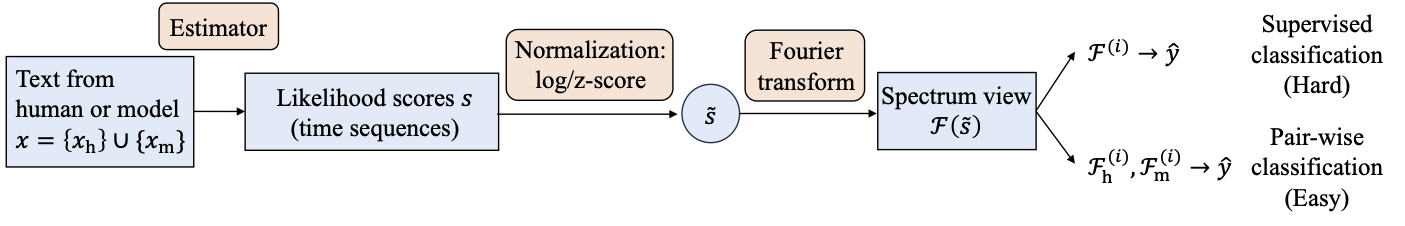
\includegraphics[width=0.5\textwidth]{images/procedure.png}
   \caption{Supervised Learning Method(Spectrum) Framework}
\end{figure}  


An augmented spectrum-based classifier is trained using frequency features obtained from multiple circularized variants of the original likelihood sequence. \textbf{This involves circularizing the sequence, applying the Fourier transform to each variant, and averaging the resulting spectra to construct a robust representation}. Inspired by circular convolution in signal processing, this method serves as a form of data augmentation to enhance weak periodic signals and improve classification performance.

\subsection{Zero-shot Detection Methods}

A \textbf{heuristic spectrum-based classifier} is proposed to distinguish human-written from machine-generated texts by leveraging \textbf{frequency-domain features}. The classification decision is based on the summed spectral power difference over a selected low-frequency range, and an empirical threshold~$\varepsilon$, according to the following criterion:
\[
\left| \sum_{k=1}^{\delta} \| X_{\text{Human}}(\omega_k) \| - \sum_{k=1}^{\delta} \| X_{\text{Model}}(\omega_k) \| \right| > \varepsilon
\]


\section{Data Preprocessing}

\textbf{English Data:}
\begin{itemize}
  \item Source:  {\footnotesize Ghostbuster dataset (https://github.com/vivek3141/ghostbuster-data)}
  \item Domains: \textbf{essay, reuter, wp}
  \item Each domain contains 6 types of LLM-generated texts and one human-written (HM) type
  \item \textbf{CSV with fields} — text, label {\footnotesize \textbf{(1 for LLM, 0 for HM)}}, domain
  \item Created mixed-domain and domain-specific CSV files
  \item Split into train, validation, test sets with ratio \textbf{8:1:1}
  \item Data cleaning applied to handle corrupted or missing entries
\end{itemize}

\textbf{Chinese Data:}
\begin{itemize}
  \item Domains: \textbf{news, webnovel, wiki}
  \item Human-written data and Qwen2-72b generated data
  \item \textbf{Same preprocessing pipeline} as English data
  \item Input format well structured; tested both \textbf{concatenated input-output} and \textbf{input only}
  \item Found better results \textbf{without concatenation} of input 
\end{itemize}




Data Preprocessing for Zero-shot Method

\begin{itemize}
  \item \textbf{Same datasets} as supervised method used for consistency
  \item For each domain, data split into \textbf{two separate text files}: one for human-written (HM), one for LLM-generated (LLM) texts
  \item Each line in txts corresponds to \textbf{one data entry} from the original dataset
  \item Related metadata such as topics and prompts stored in separate files, \textbf{aligned by line number} across HM and LLM files
  \item Missing or anomalous values identified and cleaned 
  \item For English data, each domain contains 6 LLM samples and 1 HM sample per topic, duplicate HM for 6 times to \textbf{balance sample counts}
\end{itemize}



Processed Data Overview


\textbf{CSV Files:}
\begin{itemize}
  \item \textbf{English Data:}
  \begin{itemize}
    \item eng\_essay.csv, eng\_reuter.csv, eng\_wp.csv
    \item eng\_hm\_essay.csv, eng\_hm\_reuter.csv, eng\_hm\_wp.csv
    \item eng\_llm\_essay.csv, eng\_llm\_reuter.csv, eng\_llm\_wp.csv
    \item eng\_mix (mixed domain)
  \end{itemize}
  \item \textbf{Chinese Data:}
  \begin{itemize}
    \item zh\_domain
    \item zh\_mix (mixed domain)
  \end{itemize}
\end{itemize}



\textbf{TXT Files:}
\begin{itemize}
  \item \textbf{English Data:}
  \begin{itemize}
    \item eng\_essay\_hm.txt, eng\_essay\_llm.txt
    \item eng\_reuter\_hm.txt, eng\_reuter\_llm.txt
    \item eng\_wp\_hm.txt, eng\_wp\_llm.txt
  \end{itemize}
  \item \textbf{Chinese Data:(similar)}
  \begin{itemize}
    \item zh\_news\_hm.txt, zh\_news\_llm.txt
    \item zh\_webnovel\_hm.txt, zh\_webnovel\_llm.txt
    \item zh\_wiki\_hm.txt, zh\_wiki\_llm.txt
  \end{itemize}
\end{itemize}



\section{Experiments}
% 实验设计和结果写在这里
\subsection{Experiment Design}
\subsubsection{Supervised Learning Method}\par
We conduct a supervised learning experiment using several pre-trained Transformer models for both English and Chinese. \textbf{The training setup includes 10 epochs, a batch size of 16, the AdamW optimizer, and log intervals of 50 steps.} The learning rates are set to \textbf{\(1 \times 10^{-7}\) for English and \(1 \times 10^{-5}\) for Chinese. }

The English models include \textbf{\texttt{bert-base-uncased}, \texttt{bert-base-multilingual-cased}, \texttt{roberta-base}, and \texttt{xlm-roberta-base}}, while the Chinese models include \textbf{\texttt{bert-base-chinese}, \texttt{xlm-roberta-base}, and \texttt{roberta-base}}. To ensure fair comparison, we control for training/validation splits, batch size, number of epochs, and optimizer settings within each language group. 

Model performance is evaluated using \textbf{five metrics: accuracy, precision, recall, F1, and AUROC}. The final step involves comparing these metrics across all models and datasets.

 We conduct both \textbf{in-domain and out-of-domain (OOD)} evaluations. For in-domain evaluation, data from the three domains (essay, reuter, wp) are combined and shuffled, then \textbf{split into training, validation, and test sets in an 8:1:1 ratio.} We compute five evaluation metrics—accuracy, precision, recall, F1, and AUROC—on the test set, reporting both overall and per-domain results. 
 
 For OOD evaluation, models are trained and validated on a single domain and tested on mixed-domain data. \textbf{Metrics are computed overall and per domain}, excluding results from the training domain to a\textbf{}void data leakage. This process is repeated for each domain as the training source.



\subsubsection{FourierGPT supervised learning experiment}

The models used in our experiments include \textbf{GPT2 variants for both English (gpt2-xl, Mistral-7B-v0.1)} and \textbf{Chinese (gpt2-chinese-cluecorpussmall, Wenzhong2.0-GPT2-3.5B-chinese). }

To ensure fair comparison, we maintain consistent spectrum generation by applying circular shifts on NLL data with a fixed interpolation length, followed by standard scaling and fixed feature selection (\(k=120\)). 

Classification is performed using an SVM with an RBF kernel and fixed hyperparameters. Evaluation metrics include accuracy, precision, recall, F1 score, and AUROC.



\subsubsection{Zero-shot detection method experiment}
The zero-shot detection experiments utilize\textbf{ GPT2 variants for English (\texttt{gpt2-xl}, Mistral-7B-v0.1) and Chinese (\texttt{gpt2-chinese-cluecorpussmall}, Wenzhong2.0-GPT2-3.5B-chinese)}. To ensure fair comparison, the same spectrum generation procedure is applied across all models, with a consistent \(k\) range and threshold \(\varepsilon = 0\). \textbf{Evaluation metrics include accuracy and the AUROC curve.}

In the detection method, a sample is classified as model-generated if
\[
\sum_{i=1}^k P_{\text{model}}(\omega_i) - \sum_{i=1}^k P_{\text{human}}(\omega_i) > \varepsilon,
\]
and as human-written otherwise. The optimal \(k \in [1,50]\) is selected by evaluating accuracy, precision, recall, and F1 for each \(k\), choosing the one with the highest accuracy.

With the selected \(k\), multiple power thresholds are tested to compute true positive and false positive rates, which form the ROC curve and enable calculation of the AUROC metric.


\section{Result}
\subsection{Supervised Learning Method}
\subsubsection{English Dataset}
\begin{figure}[H]
    \centering
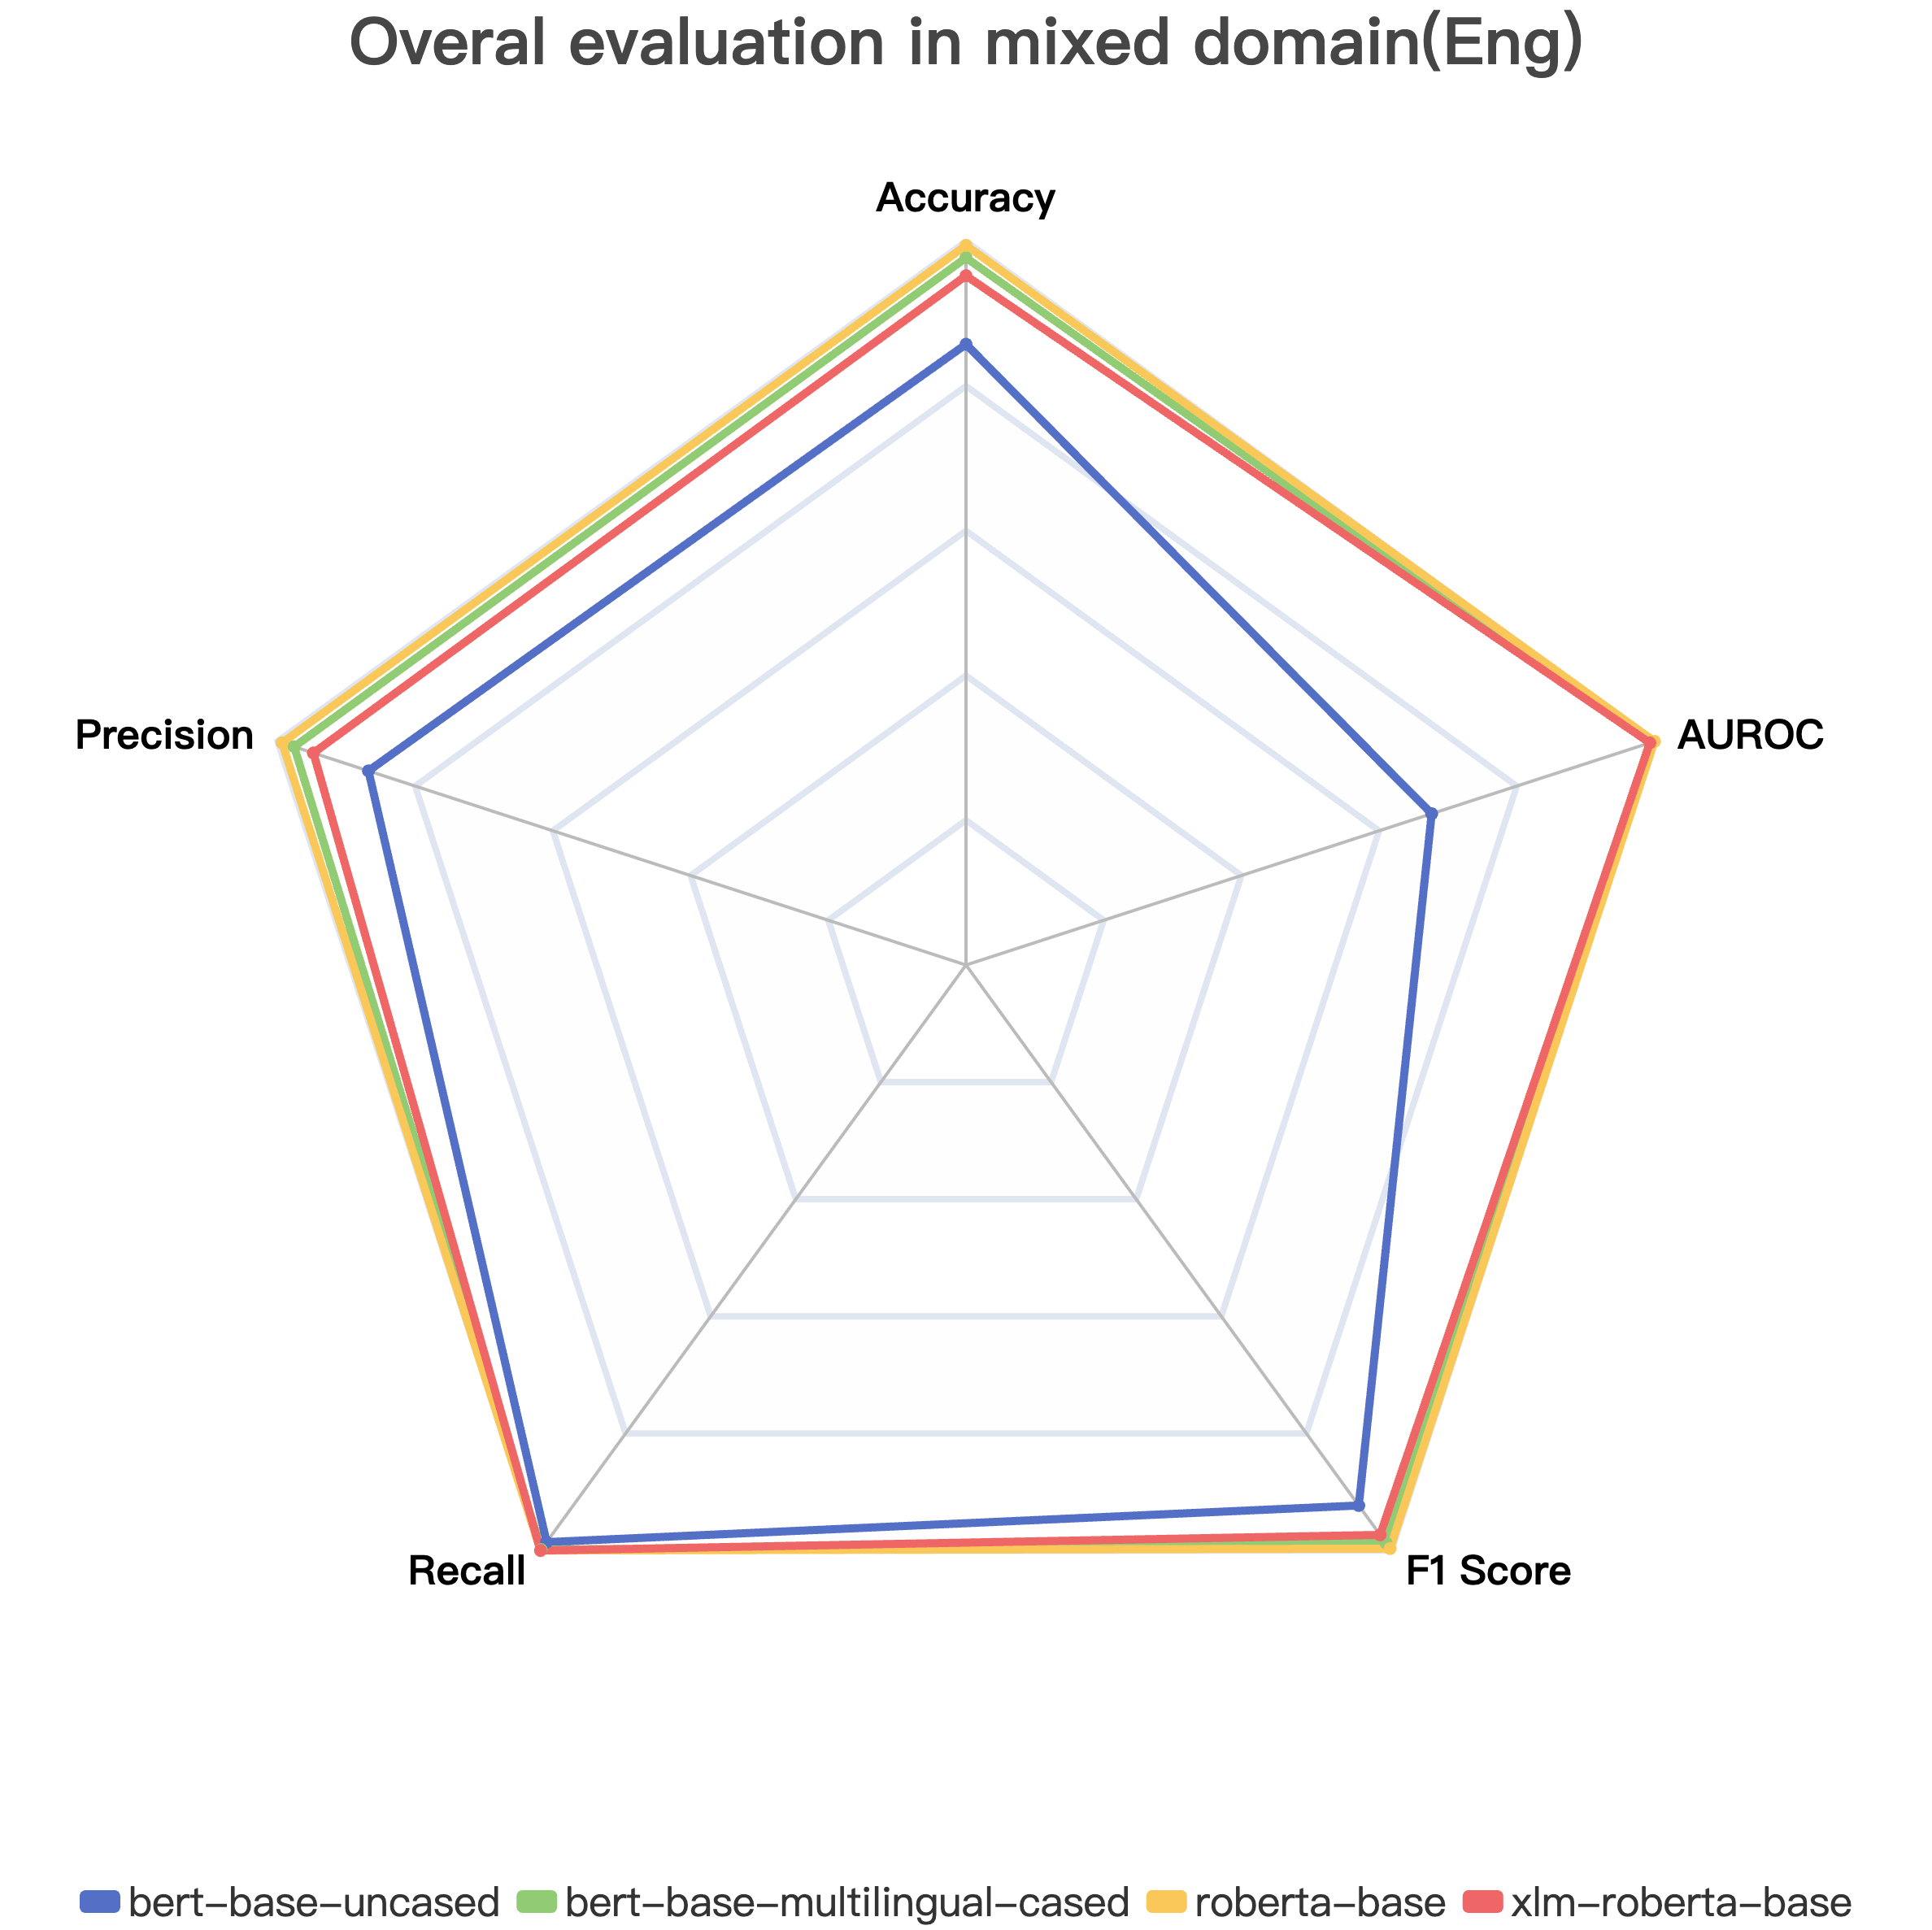
\includegraphics[width=0.3\textwidth]{images/Overal evaluation in mixed domain(Eng).png}
\caption{Overal evaluation in mixed domain(Eng)}
\end{figure} 	

In the English mixed domain, \textbf{roberta-base and xlm-roberta-base} outperform bert-base-uncased and bert-base-multilingual-cased in accuracy, F1 score, and AUROC.


\begin{figure}[H]\centering
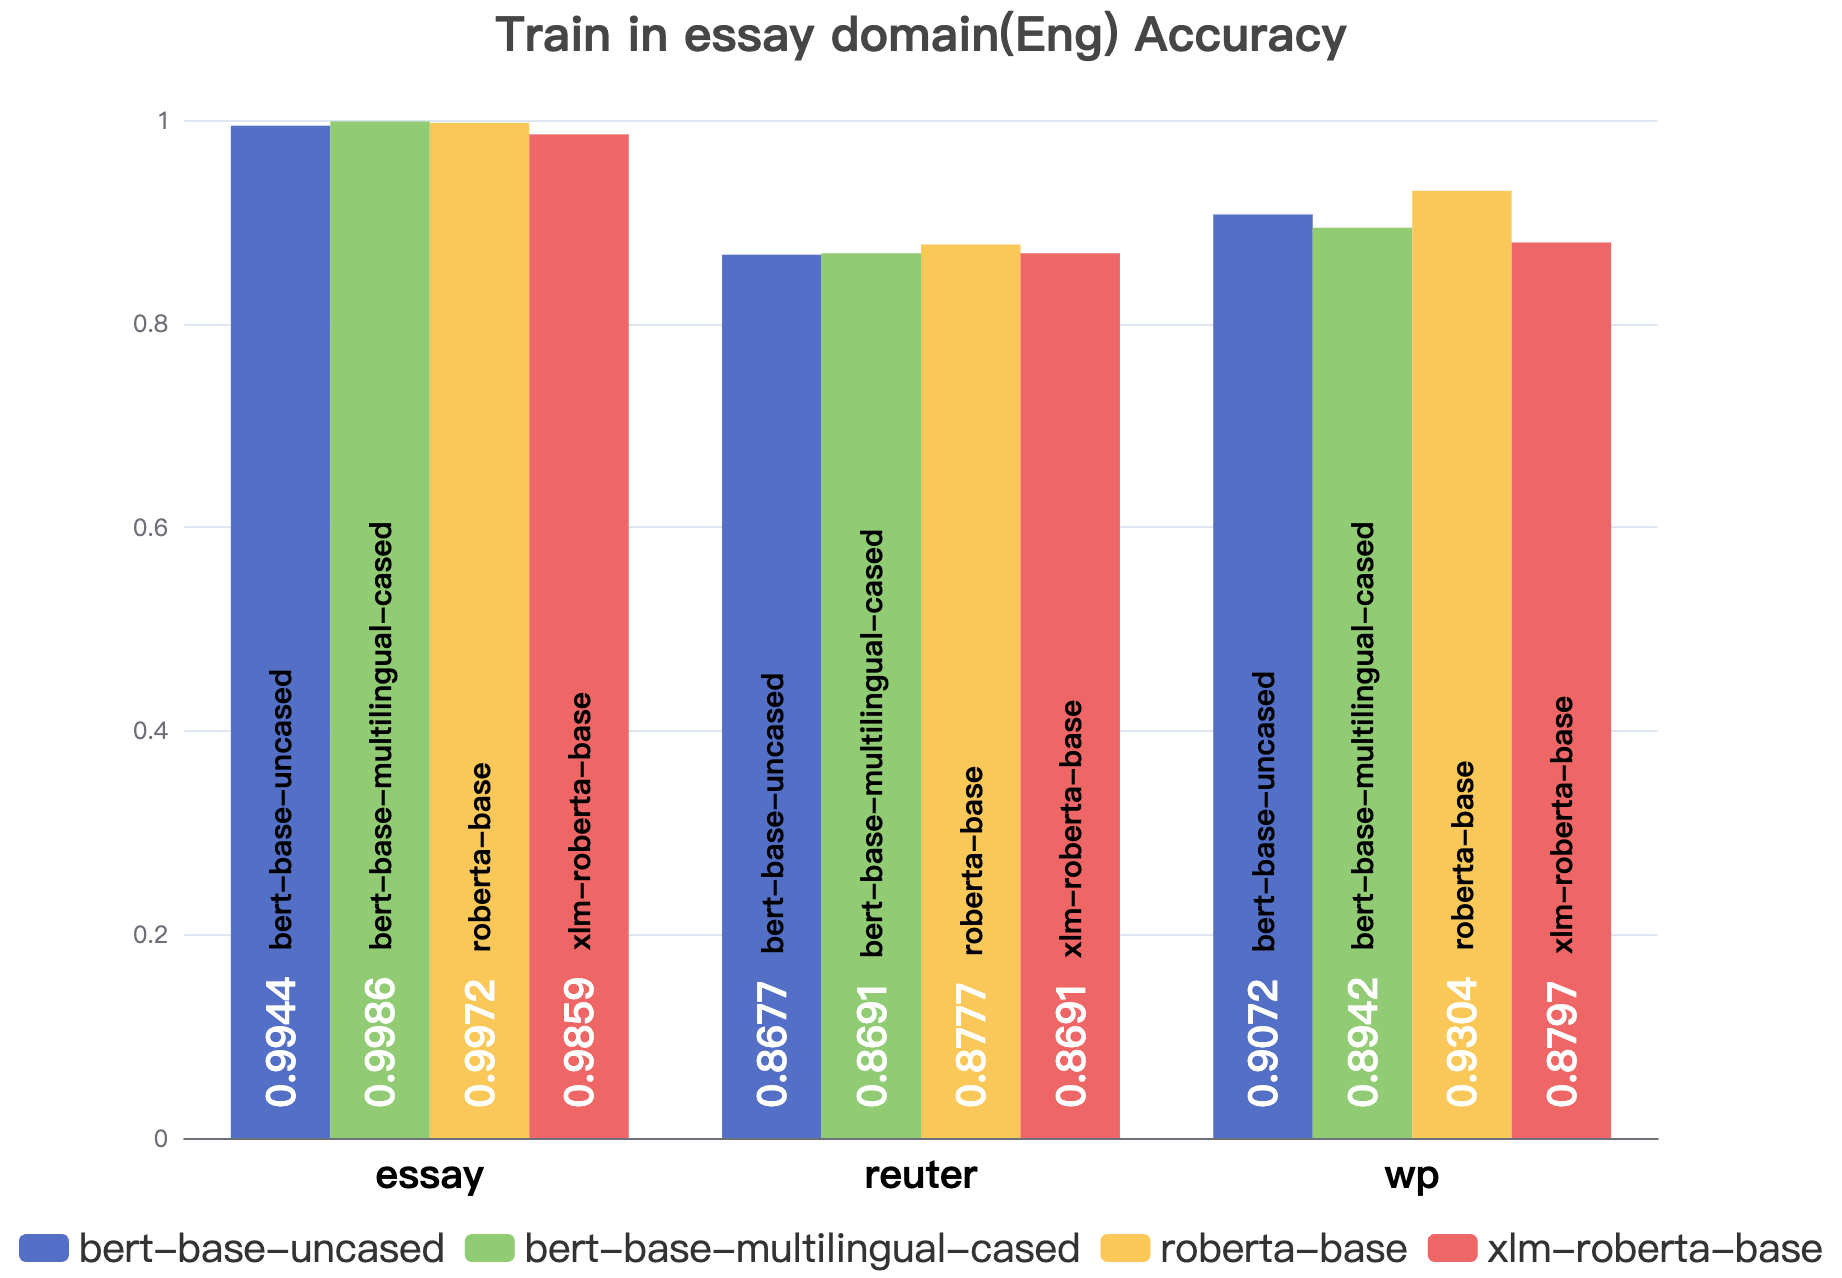
\includegraphics[width=0.6\linewidth]{images/Train in essay domain(Eng) Accuracy.png}
\caption{Accuracy in essay domain(Eng)}
    \end{figure} 	

  \begin{figure}[H]\centering
    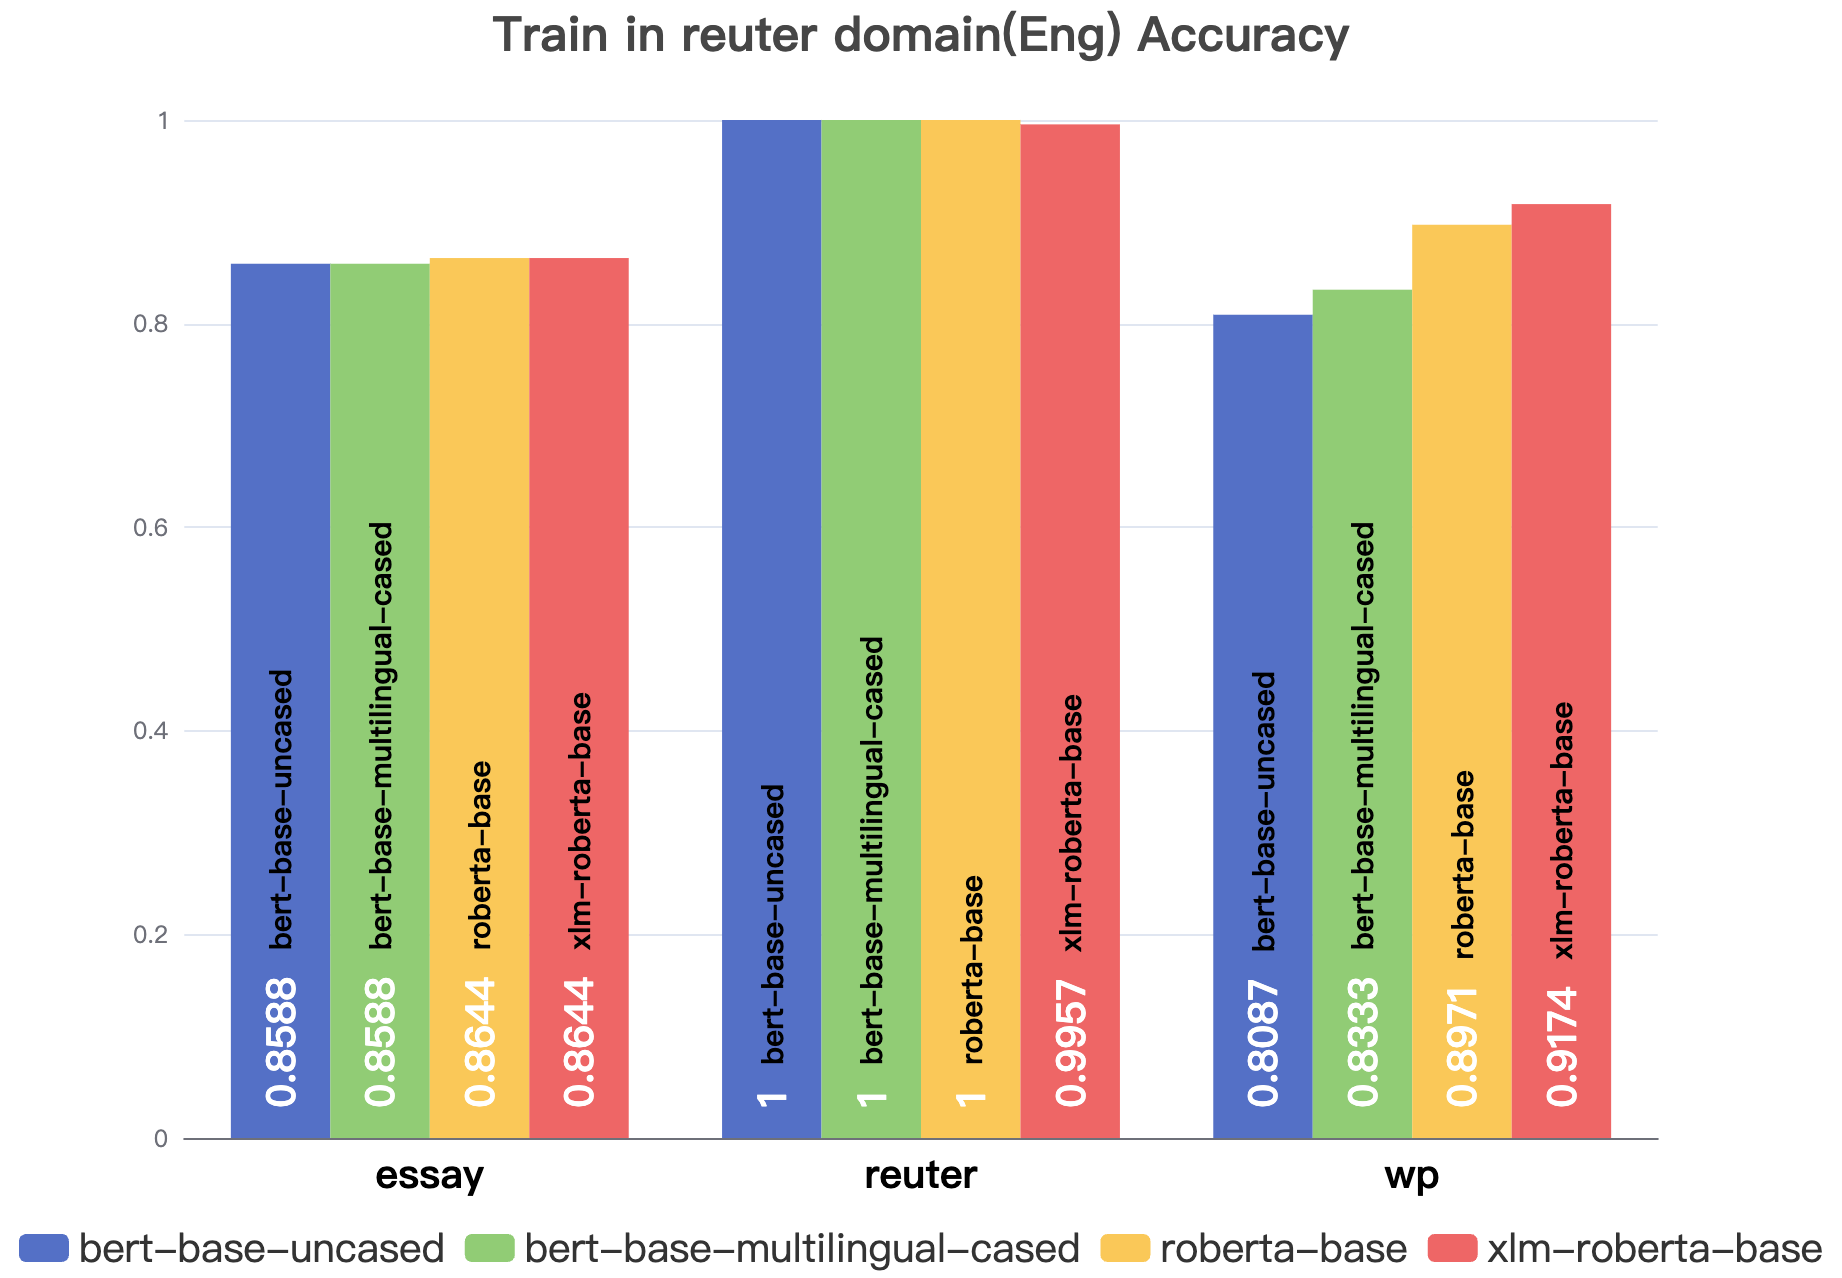
\includegraphics[width=0.6\linewidth]{images/Train in reuter domain(Eng) Accuracy.png}
    \caption{Accuracy in reuter domain(Eng)}
    \end{figure} 	

  \begin{figure}[H]\centering
    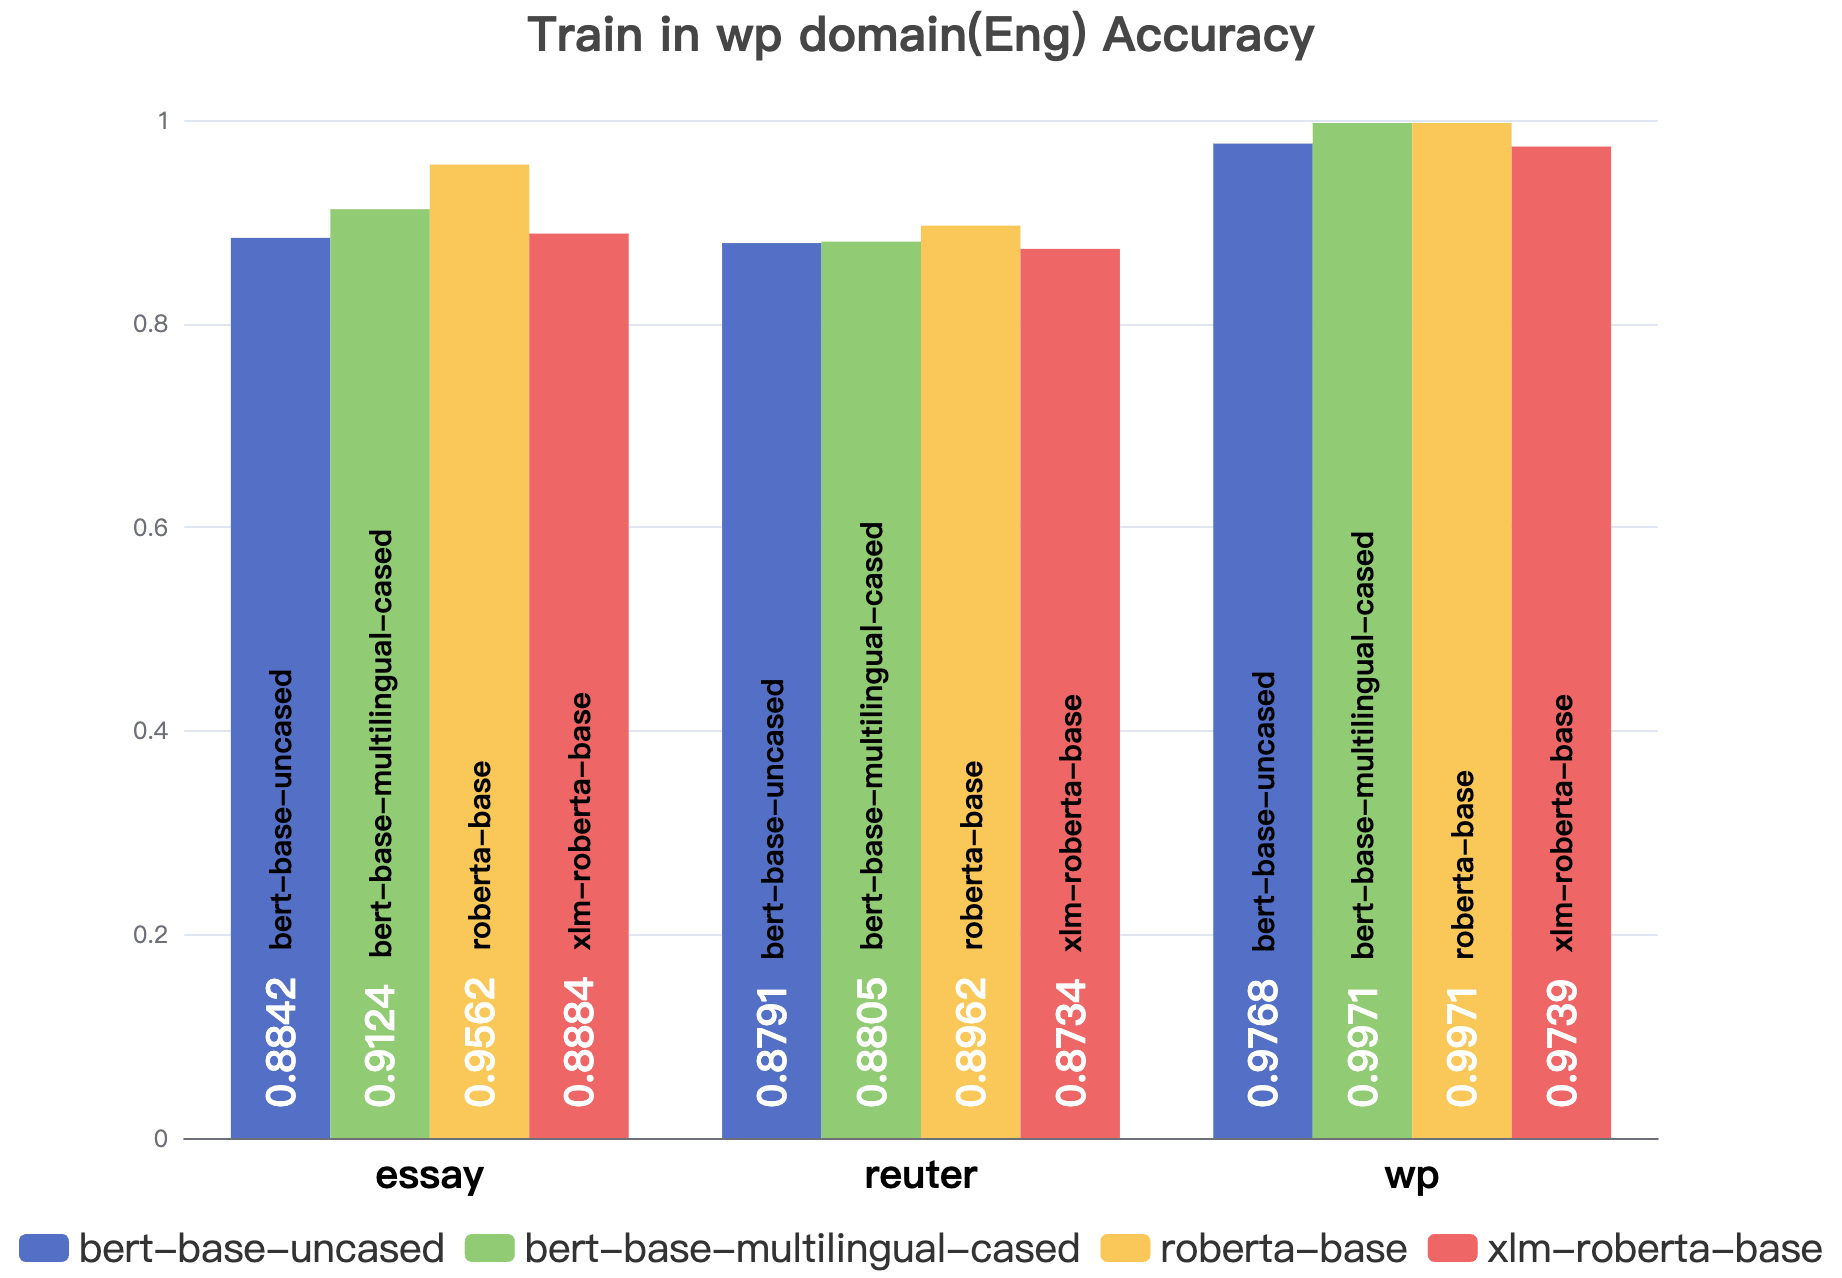
\includegraphics[width=0.6\linewidth]{images/Train in wp domain(Eng) Accuracy.png}
    \caption{Accuracy in wp domain(Eng)}
    \end{figure} 	

The models perform well within their \textbf{own training domain}, achieving accuracy generally \textbf{above 0.88}. However, accuracy significantly decreases when \textbf{tested on other domains}, often dropping \textbf{below 0.80}. Among the four models, \textbf{roberta-base} demonstrates relatively better generalization across different domains.

\begin{figure}[H]
    \centering
    \subfloat[Eng-mix]{
        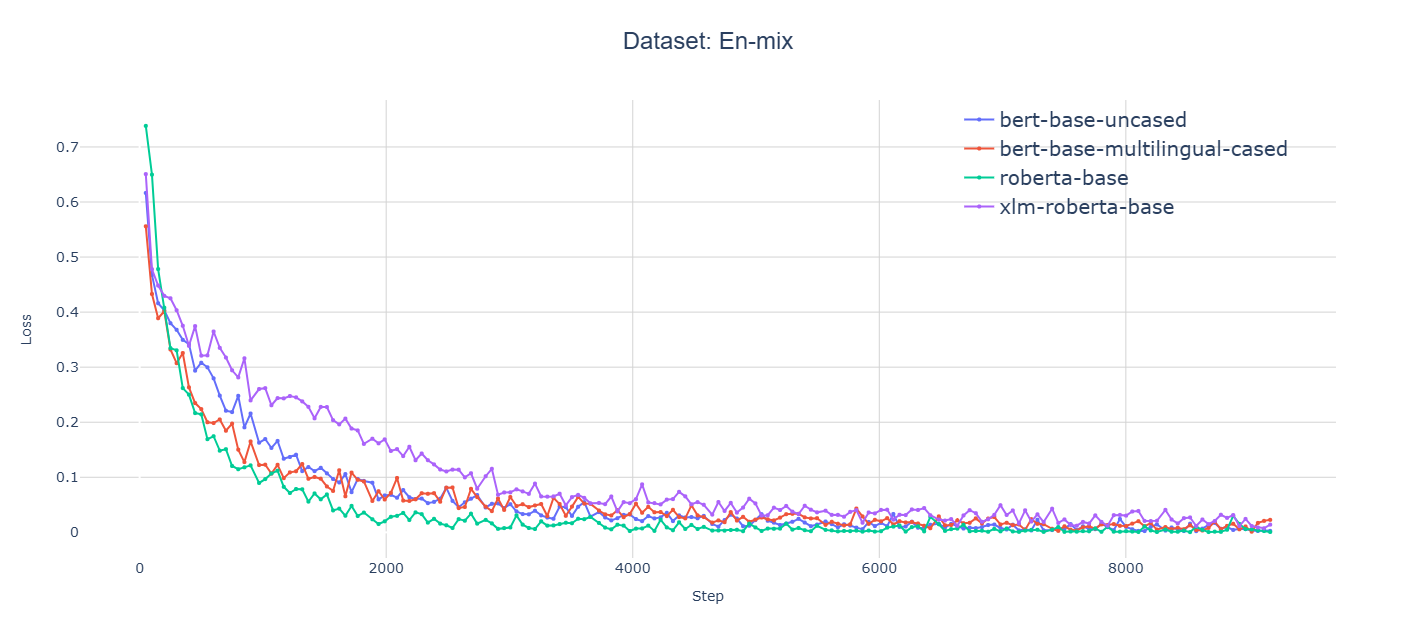
\includegraphics[width=0.6\linewidth]{images/en_mix.png}}\\
    \subfloat[Eng-essay]{
        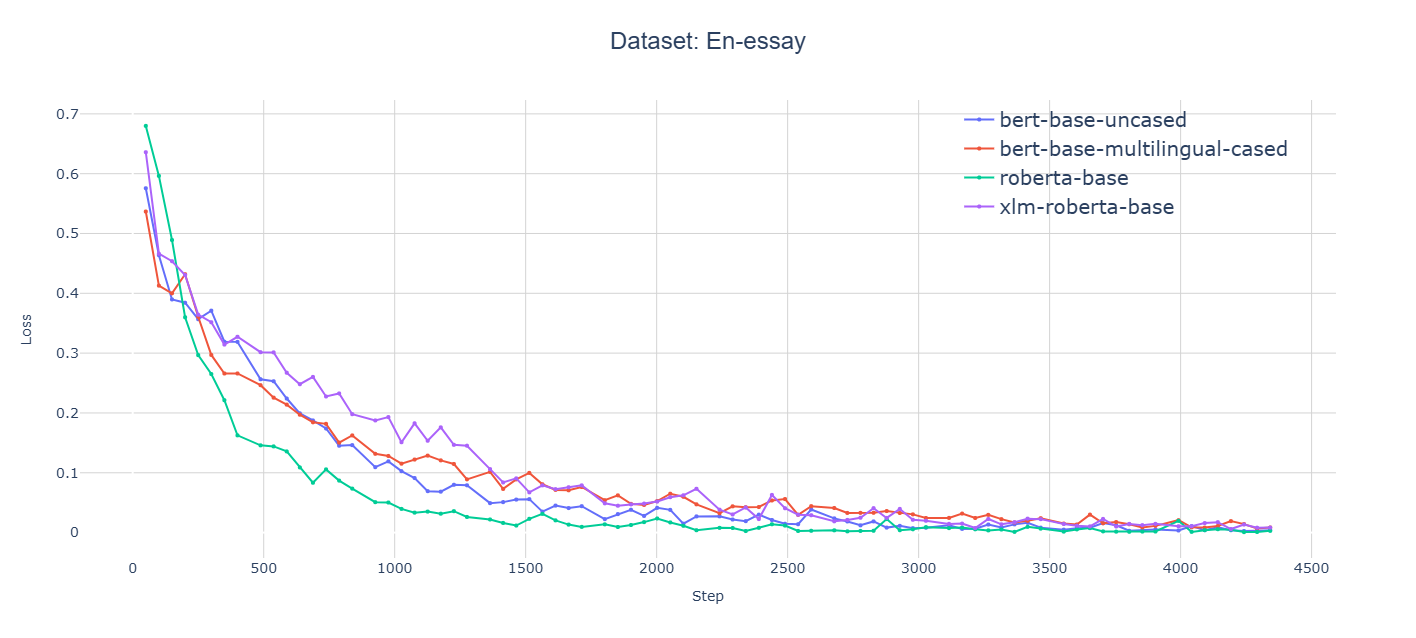
\includegraphics[width=0.6\linewidth]{images/en_essay.png}}\\
    \subfloat[Eng-reuter]{
        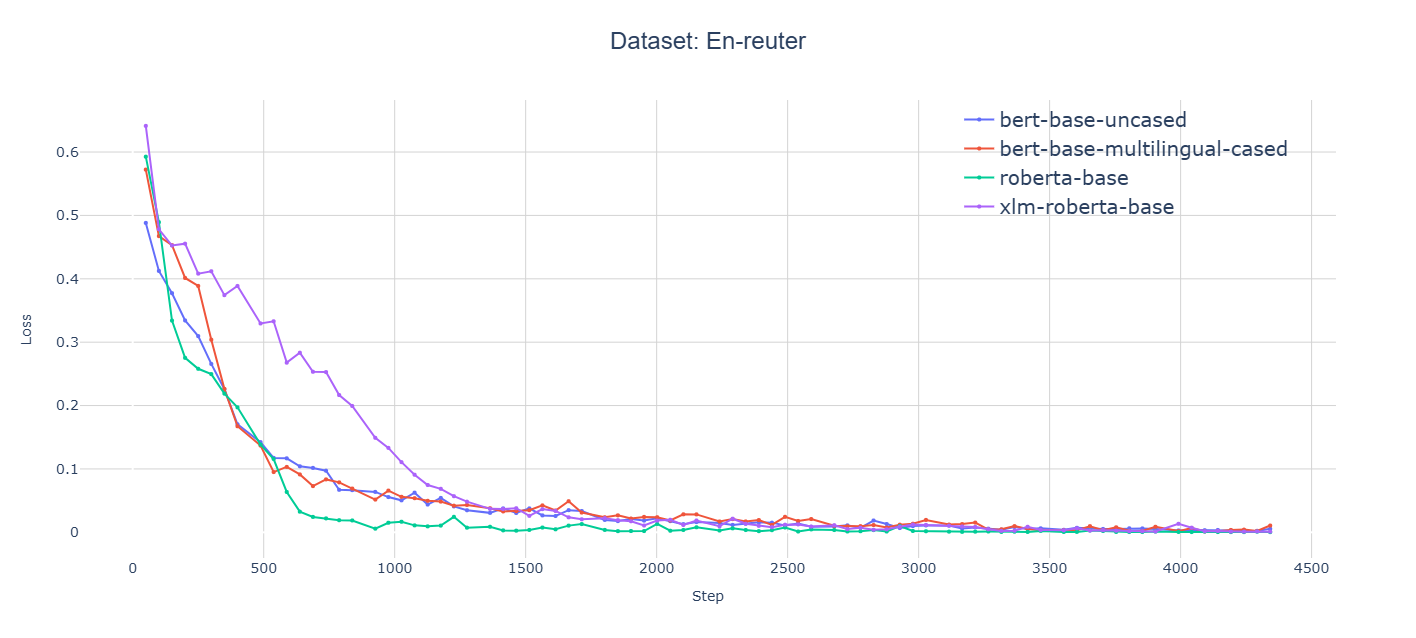
\includegraphics[width=0.6\linewidth]{images/en_reuter.png}}\\
    \subfloat[Eng-wp]{
        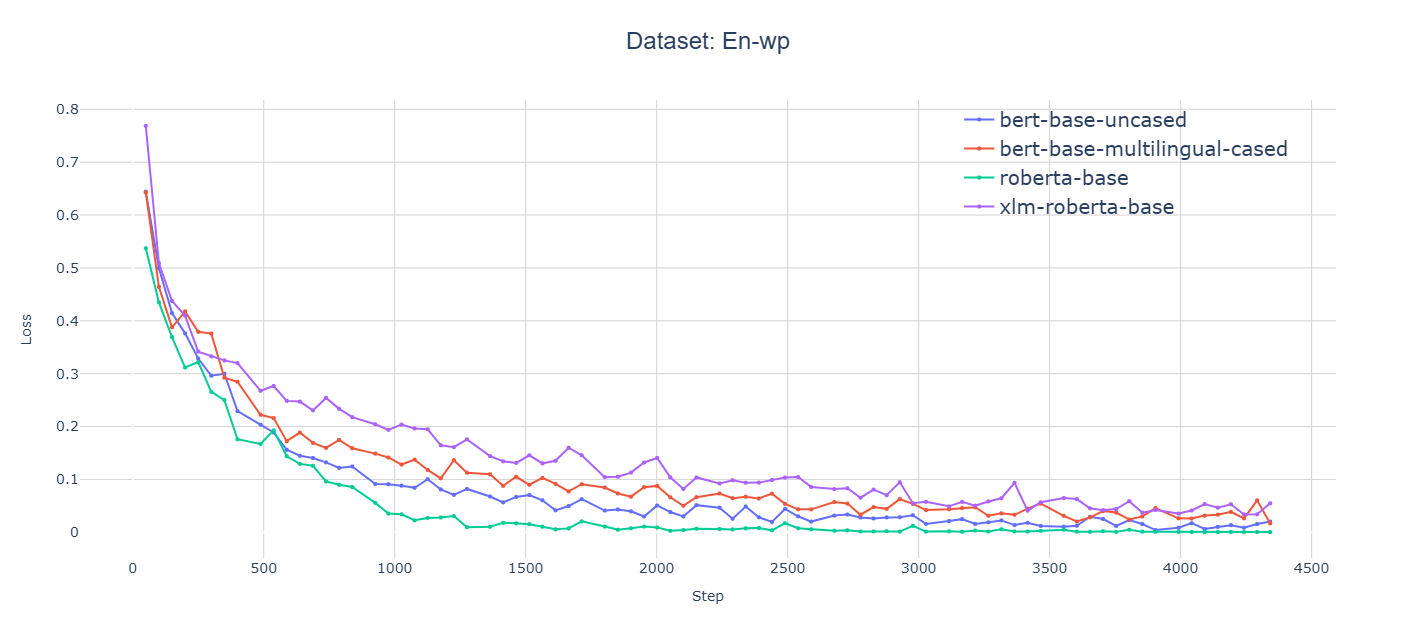
\includegraphics[width=0.6\linewidth]{images/en_wp.png}}
        \caption{Supervised Learning Method: Loss Curve (Eng)}
    \end{figure}
 
Among the four models, \textbf{roberta-base} exhibits the fastest loss decline across all datasets. Eventually, all models \textbf{converge and stabilize} with the loss values near \textbf{0.005 to 0.001}, indicating effective training and good convergence behavior.




In the supervised learning method, we compare model performance across English datasets using multiple evaluation metrics.


\begin{table}[H]
    \centering
    \caption{bert-base-uncased (Eng) overall/essay/reuter/wp}
    \label{tab:my_label}
  \setlength{\tabcolsep}{2pt}
\renewcommand{\arraystretch}{1.0}
\resizebox{0.5\textwidth}{!}{%
\begin{tabular}{|l|c|c|c|c|}
\hline
\textbf{FT domain} & \textbf{mixed} & \textbf{essay} & \textbf{reuter} & \textbf{wp} \\
\hline
Accuracy & 
0.8577 / 0.8460 / 0.8578 / 0.8696 & 
0.9234 / 0.9944 / 0.8677 / 0.9072 & 
0.8896 / 0.8588 / 1.0000 / 0.8087 & 
0.9129 / 0.8842 / 0.8791 / 0.9768 \\
\hline
Precision & 
0.8679 / 0.8640 / 0.8590 / 0.8813 & 
0.9291 / 0.9935 / 0.8889 / 0.9091 & 
0.9421 / 0.8657 / 1.0000 / 0.9797 & 
0.9107 / 0.8829 / 0.8811 / 0.9742 \\
\hline
Recall & 
0.9857 / 0.9755 / 0.9983 / 0.9834 & 
0.9868 / 1.0000 / 0.9669 / 0.9934 & 
0.9297 / 0.9902 / 1.0000 / 0.7980 & 
0.9973 / 0.9984 / 0.9934 / 1.0000 \\
\hline
F1 Score & 
0.9231 / 0.9163 / 0.9234 / 0.9296 & 
0.9571 / 0.9967 / 0.9262 / 0.9494 & 
0.9358 / 0.9238 / 1.0000 / 0.8796 & 
0.9520 / 0.9371 / 0.9339 / 0.9869 \\
\hline
AUROC & 
0.6764 / 0.6967 / 0.5726 / 0.8464 & 
0.9526 / 0.9999 / 0.9178 / 0.9474 & 
0.8558 / 0.8016 / 1.0000 / 0.9022 & 
0.9435 / 0.8843 / 0.8828 / 1.0000 \\
\hline
\end{tabular}%
}  
\end{table}




\begin{table}[H]
 \centering
    \caption{bert-base-multilingual (Eng) overall/essay/reuter/wp}
    \label{tab:my_label}
\resizebox{0.5\textwidth}{!}{%
\begin{tabular}{|l|c|c|c|c|}
\hline
\textbf{FT domain} & \textbf{mixed} & \textbf{essay} & \textbf{reuter} & \textbf{wp} \\
\hline
Accuracy & 
0.9772 / 0.9774 / 0.9844 / 0.9696 & 
0.9210 / 0.9986 / 0.8691 / 0.8942 & 
0.8977 / 0.8588 / 1.0000 / 0.8333 & 
0.9296 / 0.9124 / 0.8805 / 0.9971 \\
\hline
Precision & 
0.9758 / 0.9760 / 0.9837 / 0.9679 & 
0.9432 / 0.9984 / 0.9051 / 0.9275 & 
0.9412 / 0.8636 / 1.0000 / 0.9785 & 
0.9553 / 0.9270 / 0.9437 / 0.9967 \\
\hline
Recall & 
0.9984 / 0.9984 / 0.9983 / 0.9983 & 
0.9670 / 1.0000 / 0.9470 / 0.9536 & 
0.9407 / 0.9935 / 1.0000 / 0.8278 & 
0.9637 / 0.9755 / 0.9156 / 1.0000 \\
\hline
F1 Score & 
0.9870 / 0.9871 / 0.9910 / 0.9829 & 
0.9550 / 0.9992 / 0.9256 / 0.9404 & 
0.9409 / 0.9240 / 1.0000 / 0.8969 & 
0.9595 / 0.9506 / 0.9294 / 0.9983 \\
\hline
AUROC & 
0.9938 / 0.9942 / 0.9948 / 0.9948 & 
0.8951 / 1.0000 / 0.8050 / 0.8857 & 
0.8161 / 0.6701 / 1.0000 / 0.9163 & 
0.9573 / 0.8957 / 0.9276 / 0.9999 \\
\hline
\end{tabular}
}
\end{table}

\begin{table}[h!]
 \centering
    \caption{roberta-base (Eng) overall/essay/reuter/wp}
    \label{tab:my_label}
\setlength{\tabcolsep}{2pt}
\renewcommand{\arraystretch}{1.0}
\resizebox{0.5\textwidth}{!}{%
\begin{tabular}{|l|c|c|c|c|}
\hline
\textbf{FT domain} & \textbf{mixed} & \textbf{essay} & \textbf{reuter} & \textbf{wp} \\
\hline
Accuracy & 
0.9943 / 0.9887 / 0.9972 / 0.9971 & 
0.9353 / 0.9972 / 0.8777 / 0.9304 & 
0.9205 / 0.8644 / 1.0000 / 0.8971 & 
0.9495 / 0.9562 / 0.8962 / 0.9971 \\
\hline
Precision & 
0.9934 / 0.9871 / 0.9967 / 0.9967 & 
0.9340 / 0.9967 / 0.8787 / 0.9330 & 
0.9160 / 0.8644 / 1.0000 / 0.8948 & 
0.9482 / 0.9532 / 0.8992 / 0.9967 \\
\hline
Recall & 
1.0000 / 1.0000 / 1.0000 / 1.0000 & 
0.9956 / 1.0000 / 0.9950 / 0.9917 & 
1.0000 / 1.0000 / 1.0000 / 1.0000 & 
0.9962 / 0.9984 / 0.9901 / 1.0000 \\
\hline
F1 Score & 
0.9967 / 0.9935 / 0.9983 / 0.9983 & 
0.9638 / 0.9984 / 0.9332 / 0.9615 & 
0.9561 / 0.9273 / 1.0000 / 0.9445 & 
0.9716 / 0.9753 / 0.9425 / 0.9983 \\
\hline
AUROC & 
1.0000 / 1.0000 / 1.0000 / 1.0000 & 
0.9797 / 1.0000 / 0.9662 / 0.9696 & 
0.9024 / 0.9039 / 1.0000 / 0.9316 & 
0.9826 / 0.9799 / 0.9392 / 1.0000 \\
\hline
\end{tabular}%
}
\end{table}



\begin{table}[h!]
 \centering
    \caption{xlm-roberta-base (Eng) overall/essay/reuter/wp}
    \label{tab:my_label}
\resizebox{0.5\textwidth}{!}{%
\begin{tabular}{|l|c|c|c|c|}
\hline
\textbf{FT domain} & \textbf{mixed} & \textbf{essay} & \textbf{reuter} & \textbf{wp} \\
\hline
Accuracy & 
0.8777 / 0.8686 / 0.8649 / 0.9000 & 
0.9119 / 0.9859 / 0.8691 / 0.8797 & 
0.9257 / 0.8644 / 0.9957 / 0.9174 & 
0.9115 / 0.8884 / 0.8734 / 0.9739 \\
\hline
Precision & 
0.8766 / 0.8691 / 0.8641 / 0.8975 & 
0.9123 / 0.9839 / 0.8678 / 0.8917 & 
0.9249 / 0.8644 / 0.9951 / 0.9253 & 
0.9093 / 0.8913 / 0.8716 / 0.9711 \\
\hline
Recall & 
0.9995 / 0.9984 / 1.0000 / 1.0000 & 
0.9940 / 1.0000 / 1.0000 / 0.9818 & 
0.9951 / 1.0000 / 1.0000 / 0.9851 & 
0.9973 / 0.9918 / 1.0000 / 1.0000 \\
\hline
F1 Score & 
0.9340 / 0.9293 / 0.9271 / 0.9460 & 
0.9514 / 0.9919 / 0.9292 / 0.9346 & 
0.9587 / 0.9273 / 0.9975 / 0.9543 & 
0.9513 / 0.9389 / 0.9314 / 0.9853 \\
\hline
AUROC & 
0.9618 / 0.9502 / 0.9653 / 0.9800 & 
0.8359 / 0.9999 / 0.6537 / 0.7428 & 
0.8115 / 0.5012 / 1.0000 / 0.9369 & 
0.9291 / 0.8743 / 0.8691 / 0.9978 \\
\hline
\end{tabular}
}
\end{table}

\subsubsection{Chinese Dataset}


\begin{figure}[H]
    \centering
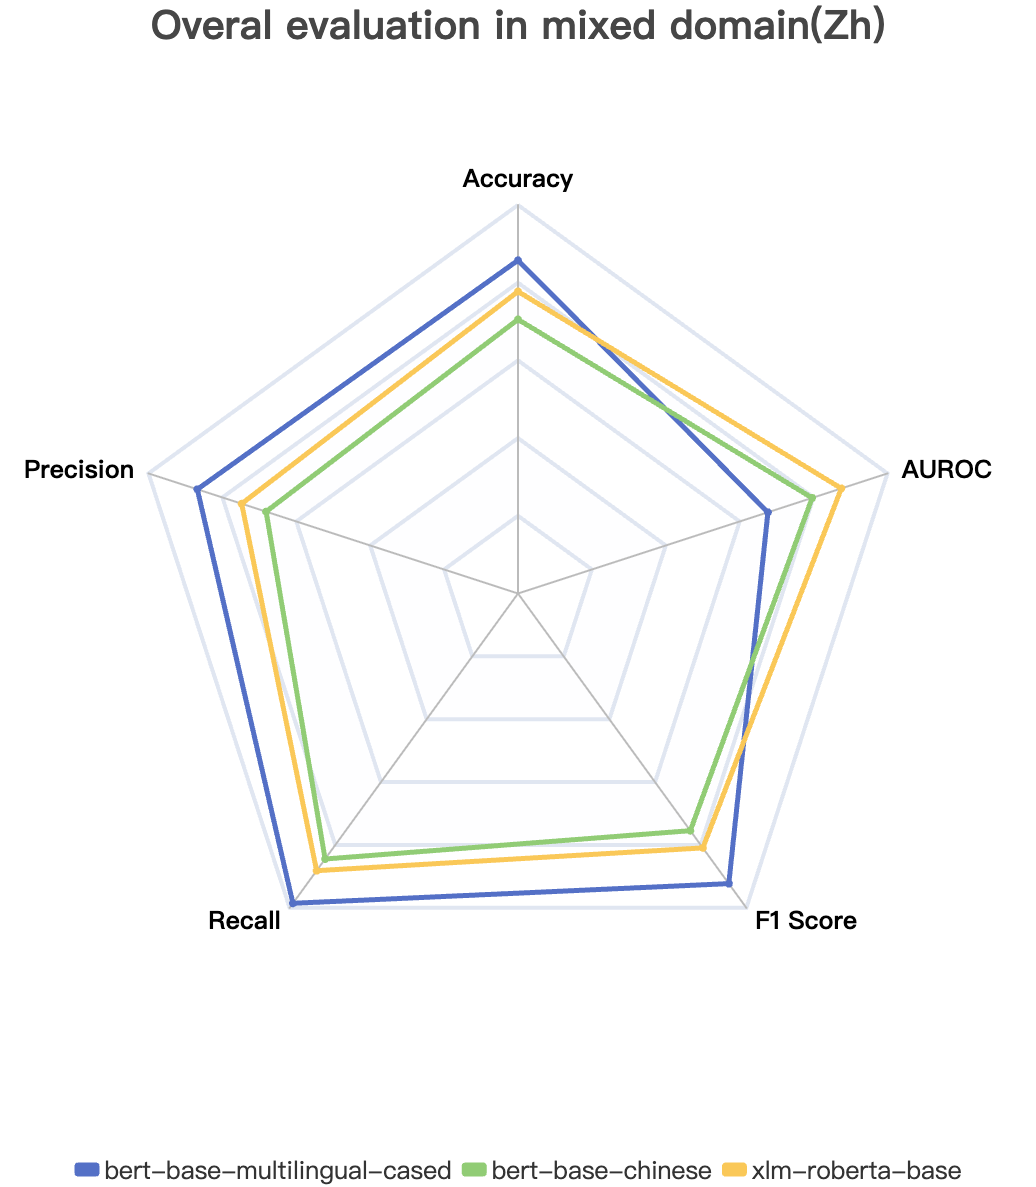
\includegraphics[width=0.3\textwidth]{images/Overal evaluation in mixed domain(Zh).png}
\caption{Overal evaluation in mixed domain(Zh)}
\end{figure}

In the Chinese mixed domain, \textbf{bert-base-multilingual-cased} achieves the highest recall and precision, while \textbf{xlm-roberta-base} leads in AUROC and F1 score, outperforming bert-base-chinese across most metrics.


\begin{figure}[H]
    \centering
    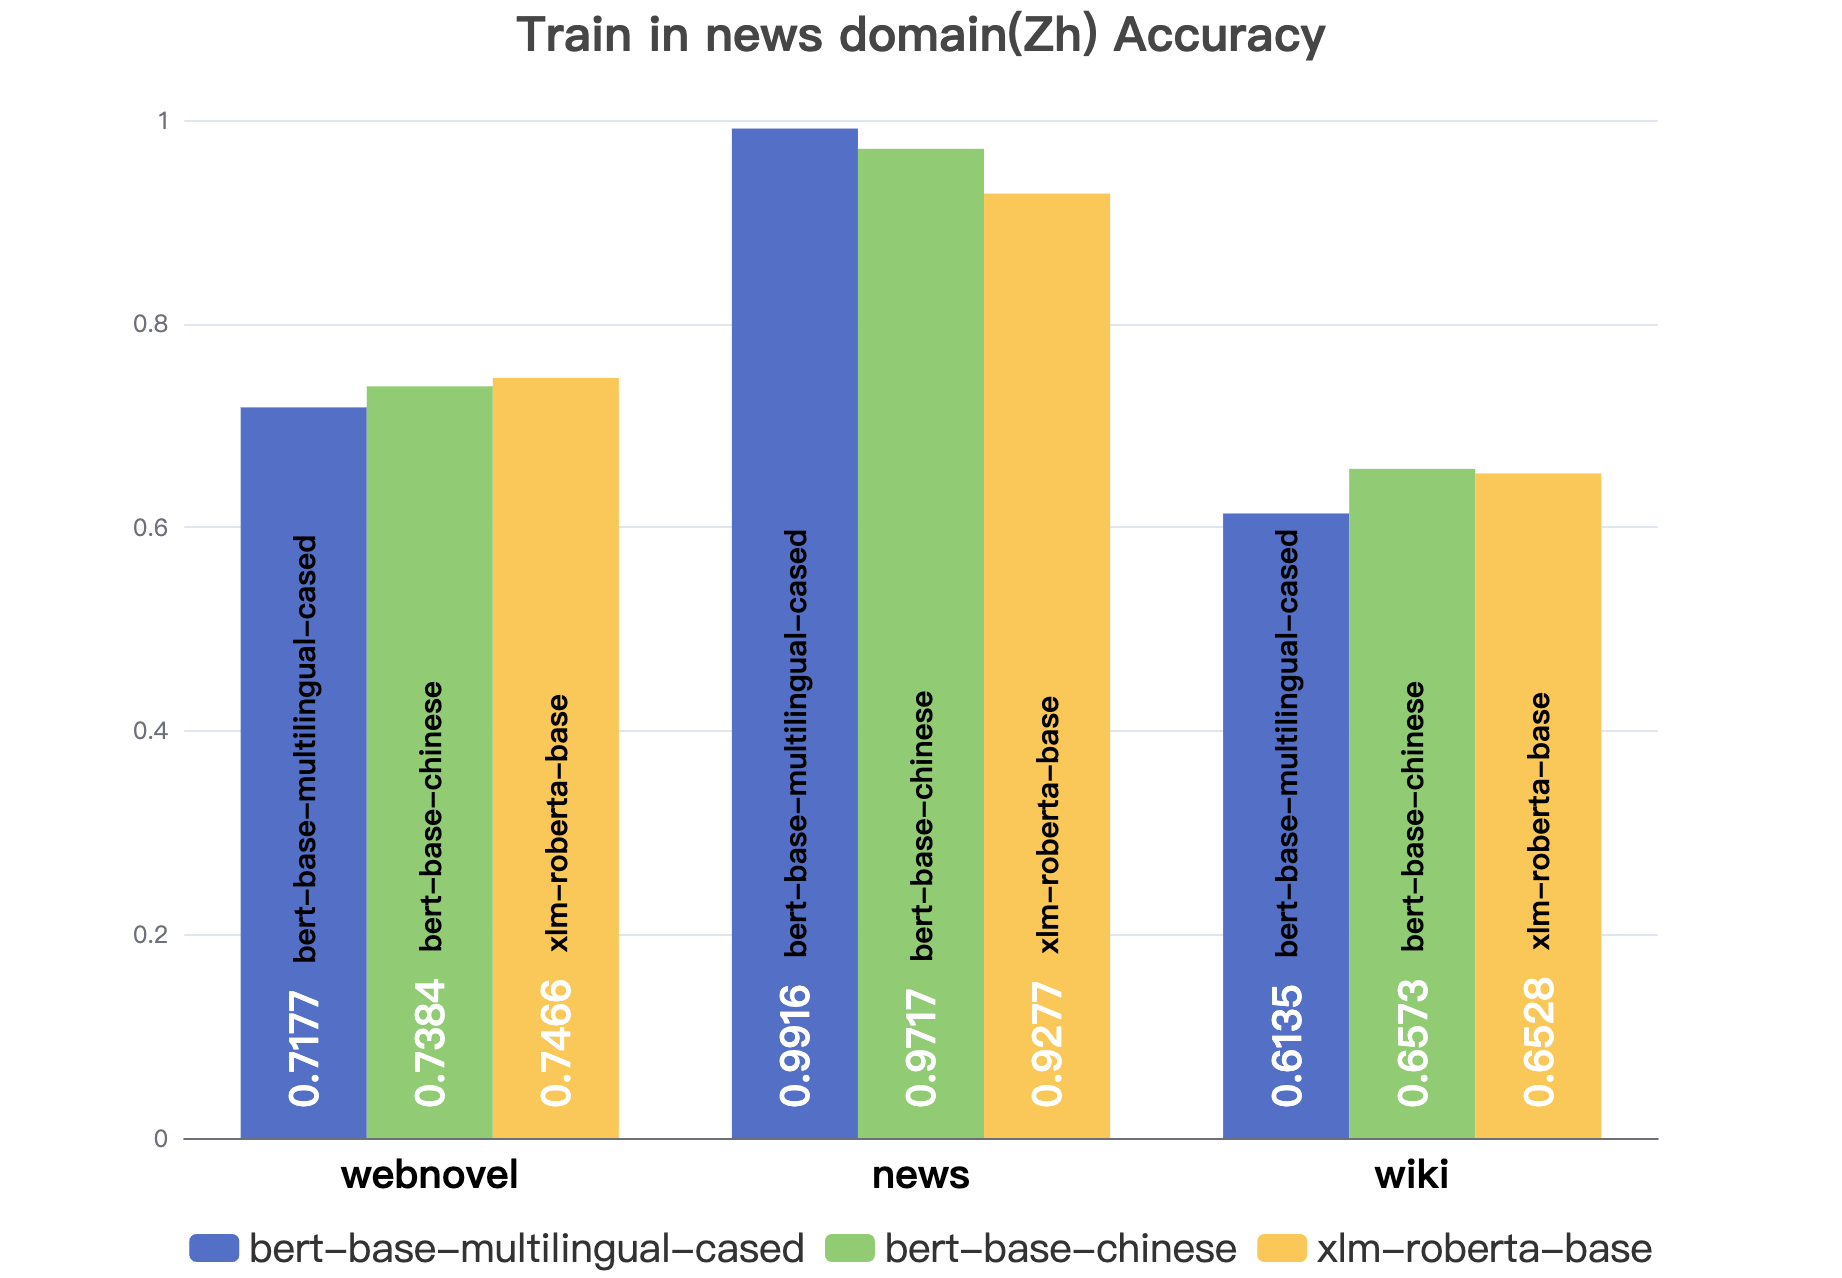
\includegraphics[width=0.8\linewidth]{images/Train in news domain(Zh) Accuracy.png}
    \caption{Accuracy in news domain(Zh)}
    \end{figure}


 \begin{figure}[H]
    \centering
    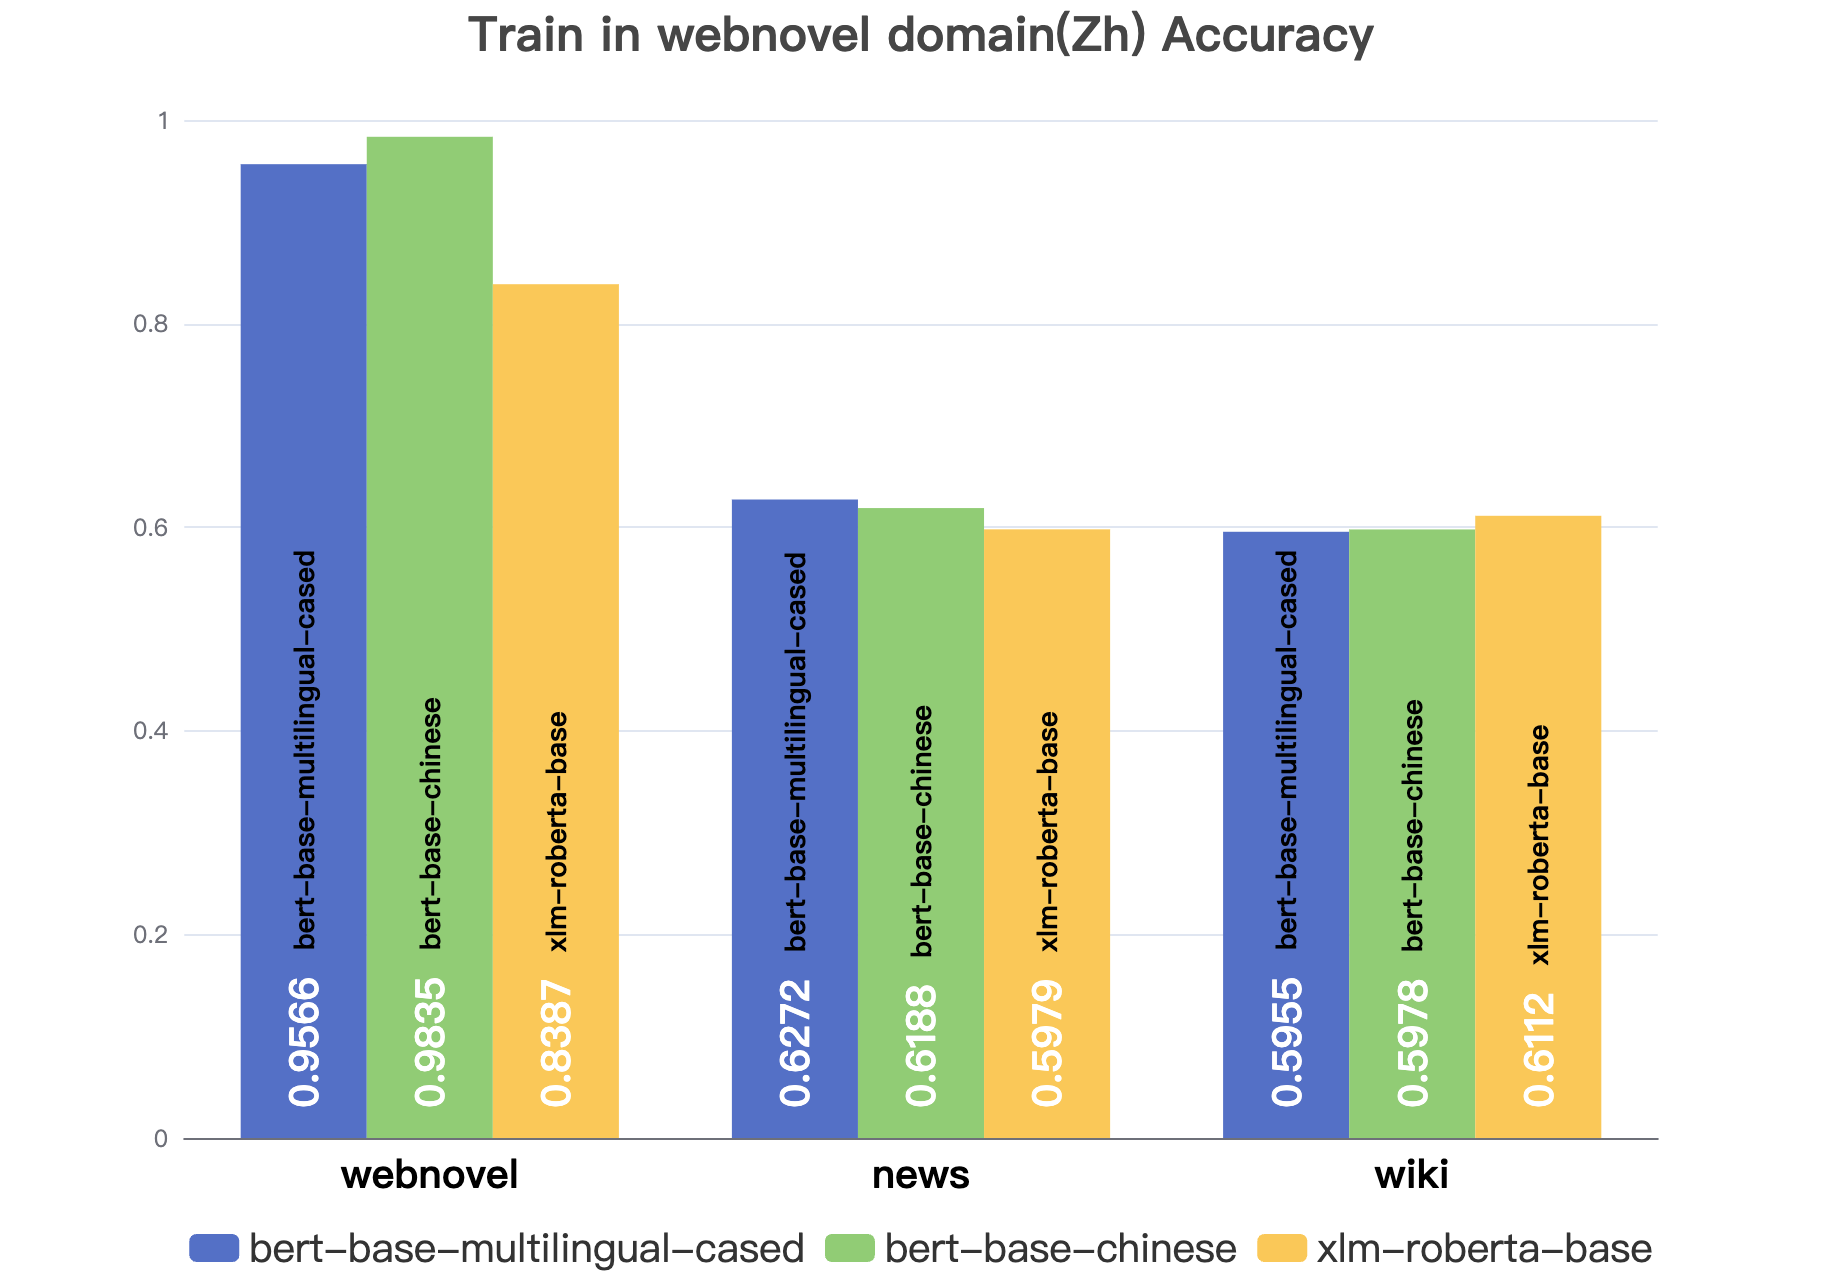
\includegraphics[width=0.8\linewidth]{images/Train in webnovel domain(Zh) Accuracy.png}
    \caption{Accuracy in webnovel domain(Zh)}
    \end{figure}

 
 \begin{figure}[H]
    \centering
    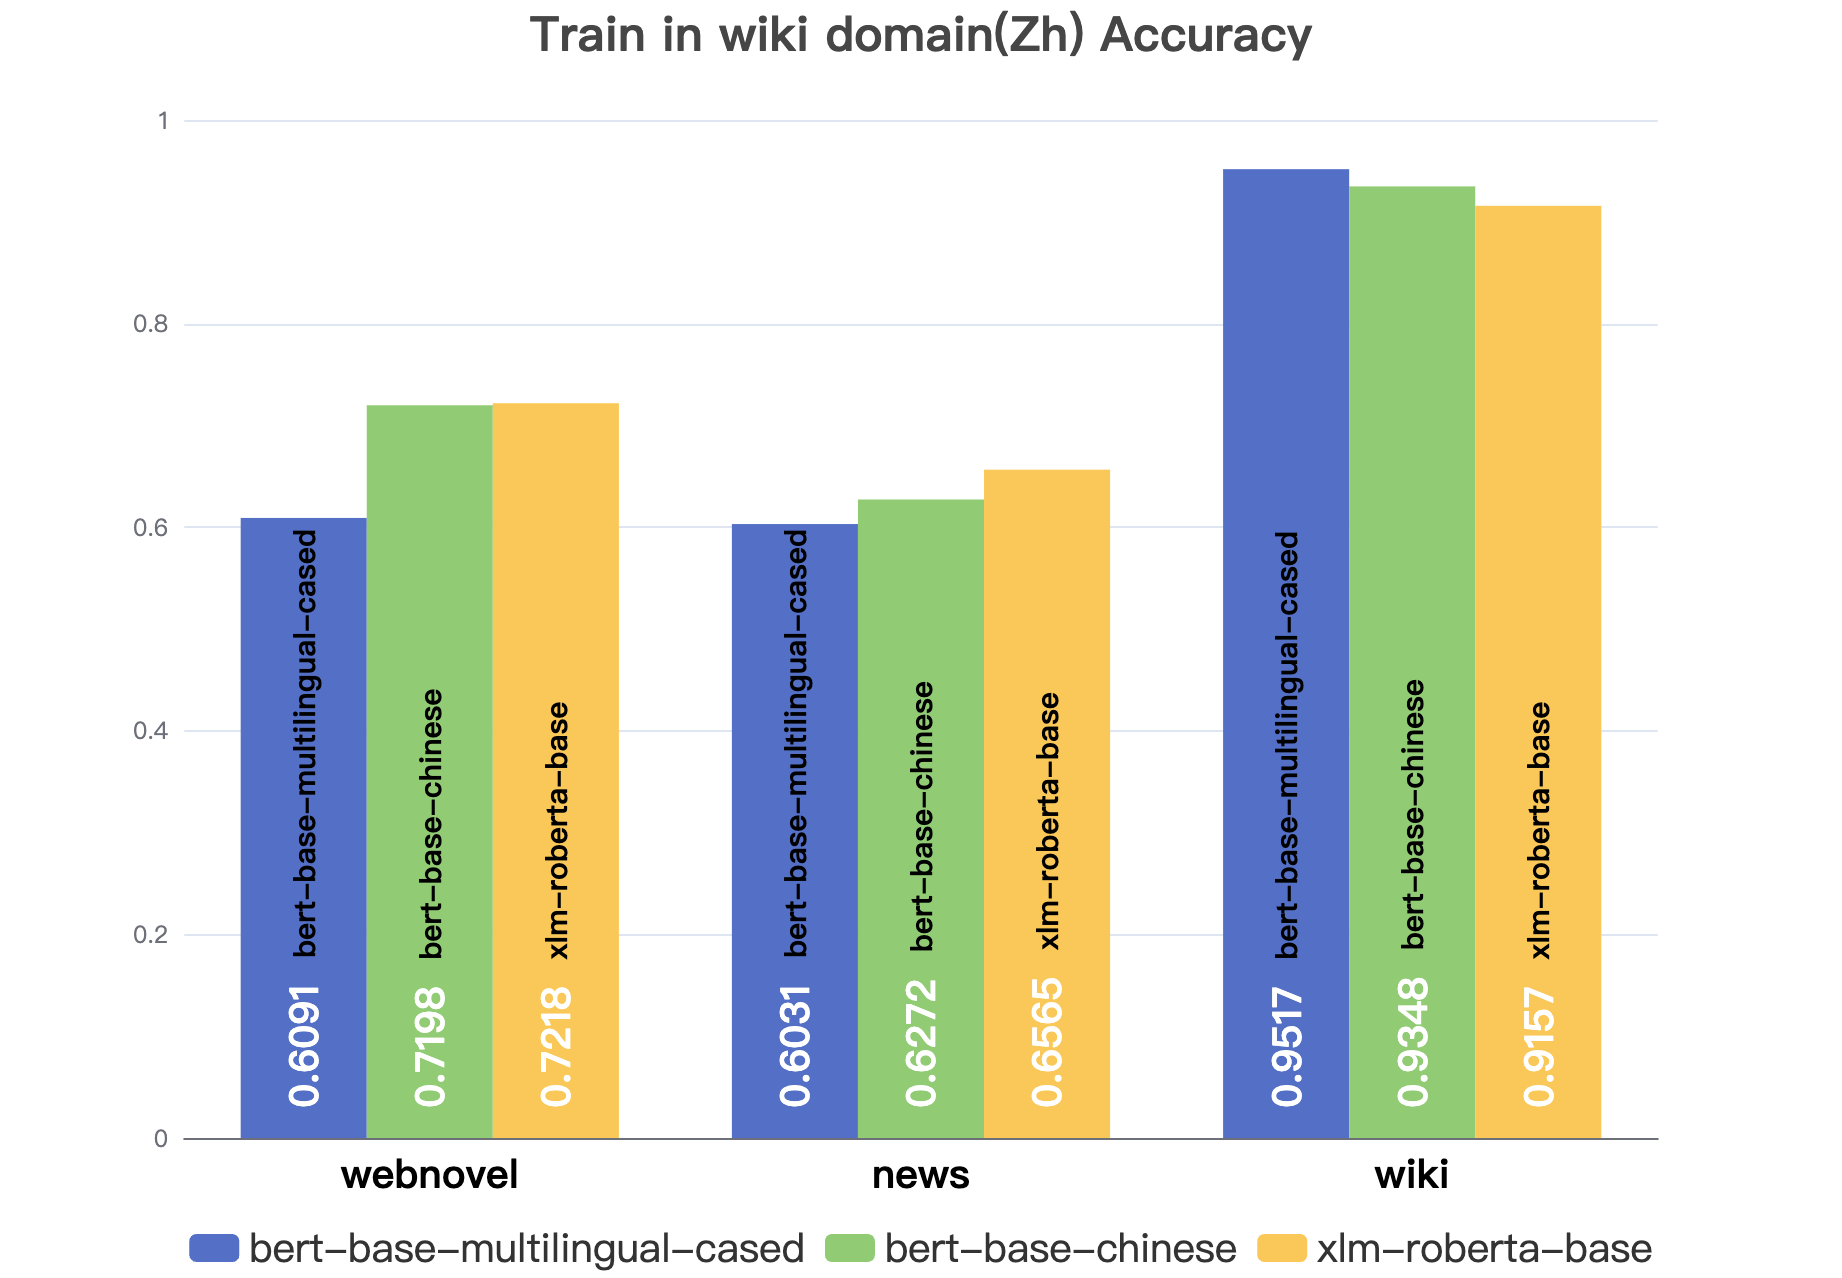
\includegraphics[width=0.8\linewidth]{images/Train in wiki domain(Zh) Accuracy.png}
    \caption{Accuracy in wiki domain(Zh)}
    \end{figure}


The models demonstrate strong performance within their \textbf{own training domain}, achieving accuracy mostly \textbf{above 0.83}. However, accuracy notably drops when \textbf{tested on other domains}, often falling between \textbf{0.63 and 0.72}. Among the three models, \textbf{bert-base-chinese} exhibits relatively better generalization across different domains.


\begin{figure}[H]
    \centering
    \subfloat[Zh-mix]{
        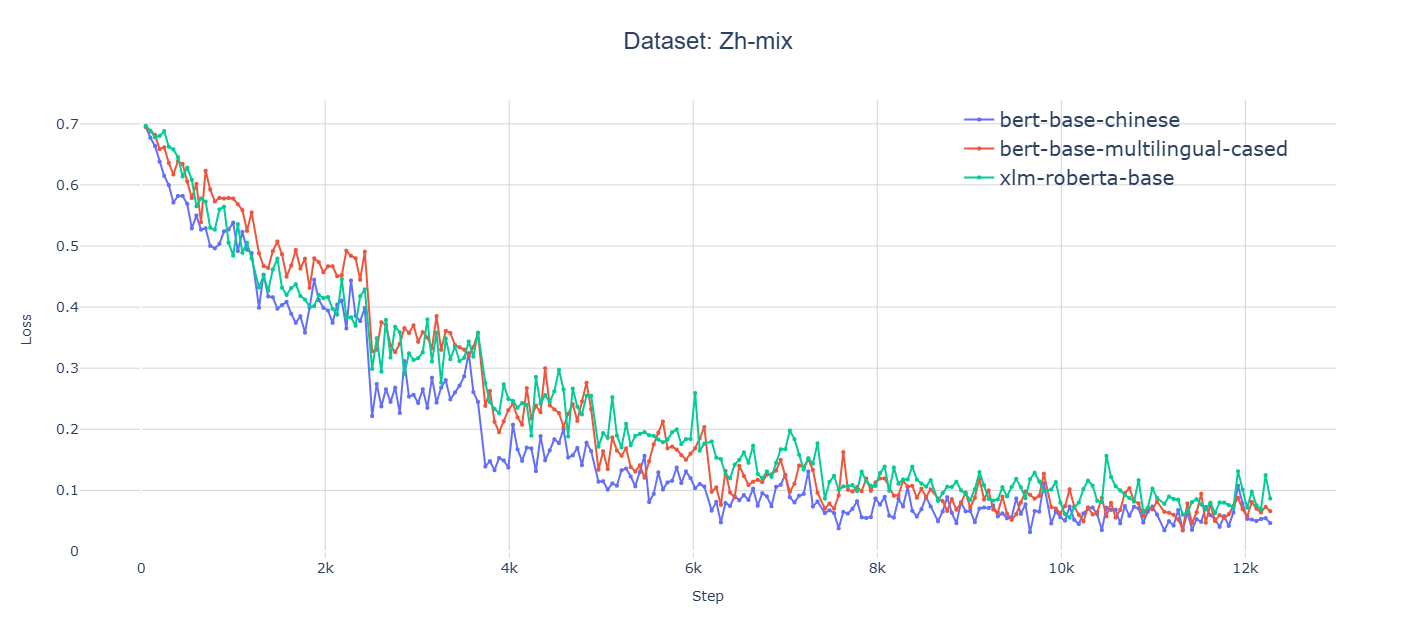
\includegraphics[width=0.8\linewidth]{images/zh-mix.png}}\\
    \subfloat[Zh-news]{
        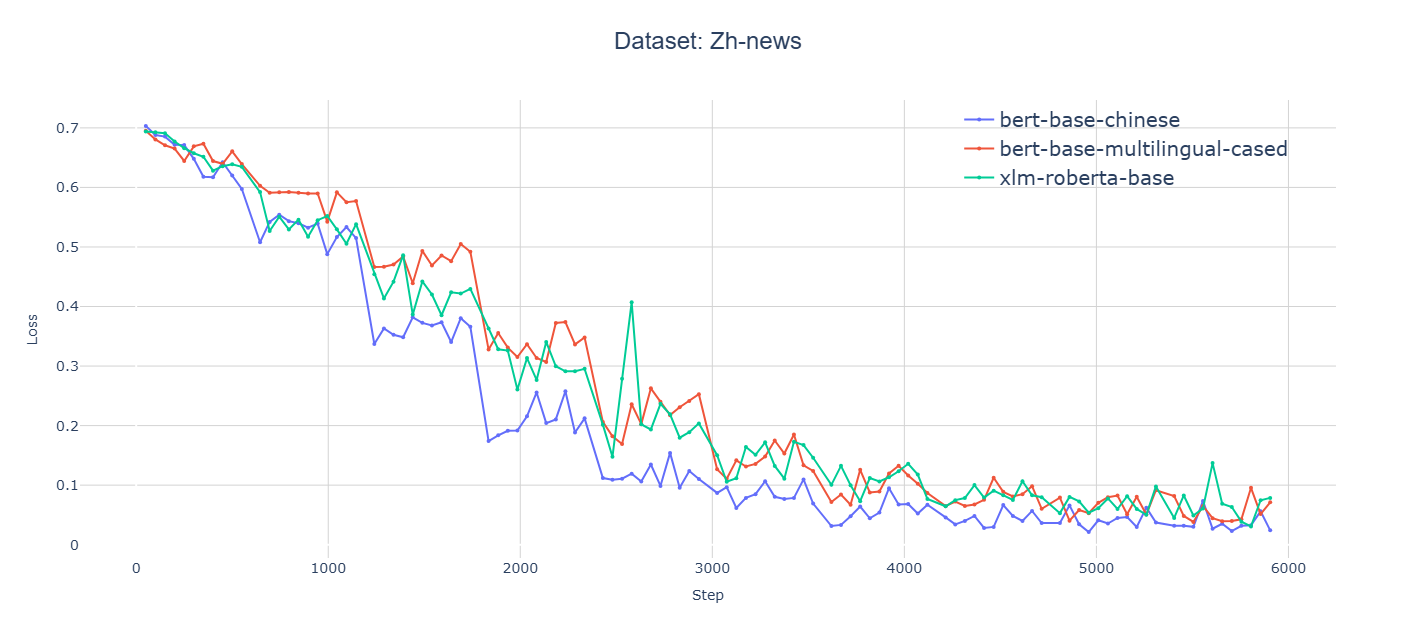
\includegraphics[width=0.8\linewidth]{images/zh-news.png}}\\
    \subfloat[Zh-webnovel]{
        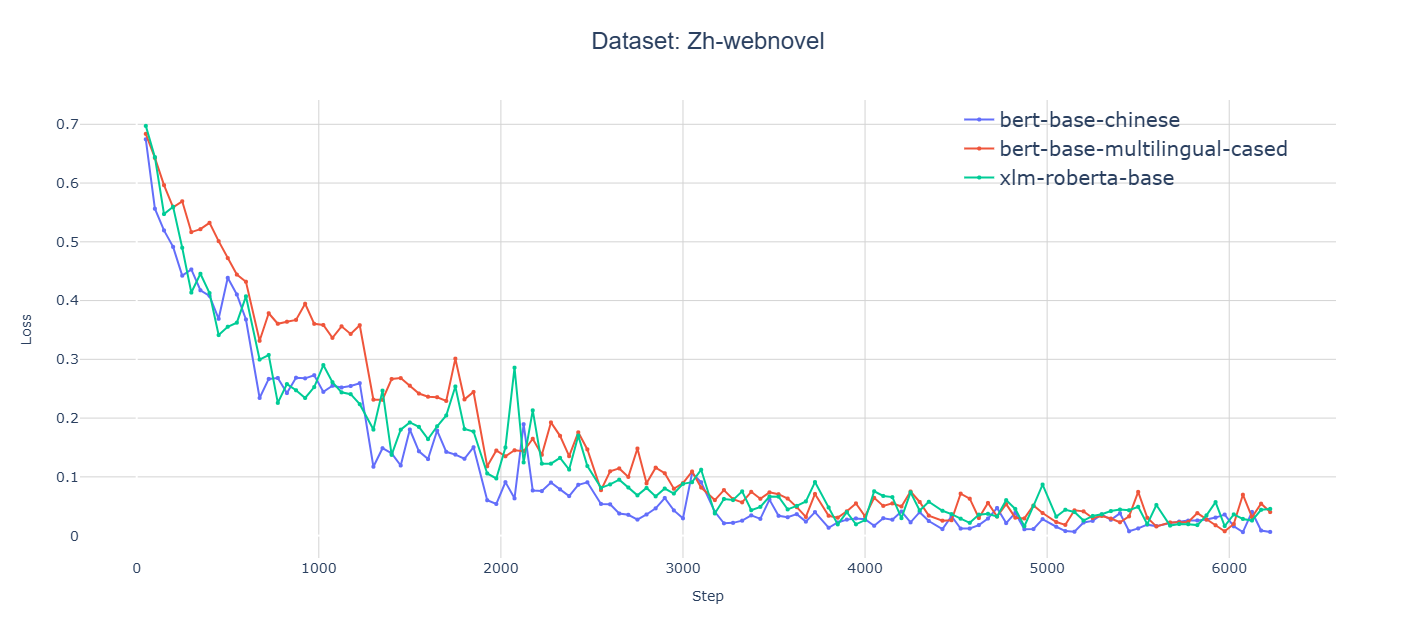
\includegraphics[width=0.8\linewidth]{images/zh-webnovel.png}}\\
    \subfloat[Zh-wiki]{
        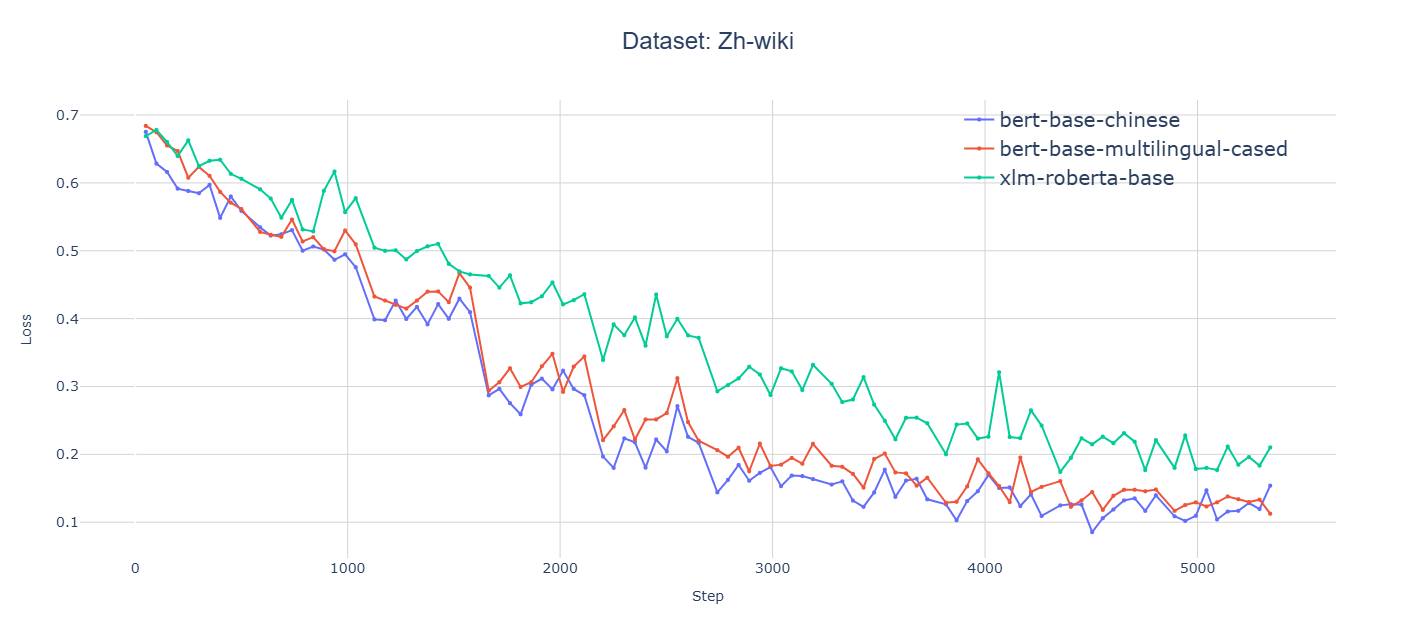
\includegraphics[width=0.8\linewidth]{images/zh-wiki.png}}
        \caption{Supervised Learning Method: Loss Curve (Zh)}
\end{figure}

Among the three models, \textbf{bert-base-chinese} shows the fastest loss decline. All models stabilize with loss values around \textbf{0.05}, demonstrating stable and effective training.

In the supervised learning method, we compare model performance across Chinese datasets using multiple evaluation metrics.


\begin{table}[H]
 \centering
    \caption{bert-base-multilingual-cased (Zh) overall/webnovel/news/wiki}
    \label{tab:my_label}
\setlength{\tabcolsep}{2pt}
\renewcommand{\arraystretch}{1.0}
% 第一个模型:bert-base-multilingual-cased (补全wiki数据)
\resizebox{0.5\textwidth}{!}{%
\begin{tabular}{|l|c|c|c|c|}
\hline
\textbf{FT domain} & \textbf{mixed} & \textbf{webnovel} & \textbf{news} & \textbf{wiki} \\
\hline
Accuracy & 
0.7055 / 0.7880 / 0.6440 / 0.6820 & 
0.7304 / 0.9566 / 0.6272 / 0.5955 & 
0.7155 / 0.6091 / 0.6031 / 0.9517 & 
0.6820 / 0.6091 / 0.6031 / 0.9517 \\
\hline
Precision & 
0.6818 / 0.7238 / 0.6289 / 0.6998 & 
0.6722 / 0.9190 / 0.5997 / 0.5952 & 
0.6924 / 0.5681 / 0.6009 / 0.9602 & 
0.6998 / 0.5681 / 0.6009 / 0.9602 \\
\hline
Recall & 
0.8447 / 0.9056 / 0.8226 / 0.8125 & 
0.9701 / 0.9979 / 0.9201 / 0.9943 & 
0.8441 / 0.7876 / 0.7778 / 0.9583 & 
0.8125 / 0.7876 / 0.7778 / 0.9583 \\
\hline
F1 Score & 
0.7546 / 0.8046 / 0.7128 / 0.7520 & 
0.7941 / 0.9568 / 0.7262 / 0.7447 & 
0.7608 / 0.6601 / 0.6780 / 0.9592 & 
0.7520 / 0.6601 / 0.6780 / 0.9592 \\
\hline
AUROC & 
0.7961 / 0.8879 / 0.6976 / 0.7649 & 
0.7528 / 0.9988 / 0.6629 / 0.5219 & 
0.7881 / 0.6637 / 0.6390 / 0.9936 & 
0.7649 / 0.6637 / 0.6390 / 0.9936 \\
\hline
\end{tabular}%
}
\end{table}



\begin{table}[H]
 \centering
    \caption{bert-base-chinese (Zh) overall/webnovel/news/wiki}
    \label{tab:my_label}
% 第二个模型:bert-base-chinese
\resizebox{0.5\textwidth}{!}{%
\begin{tabular}{|l|c|c|c|c|}
\hline
\textbf{FT domain} & \textbf{mixed} & \textbf{webnovel} & \textbf{news} & \textbf{wiki} \\
\hline
Accuracy & 
0.7219 / 0.7942 / 0.6754 / 0.6933 & 
0.7376 / 0.9835 / 0.6188 / 0.5978 & 
0.7920 / 0.7384 / 0.9717 / 0.6573 & 
0.7564 / 0.7198 / 0.6272 / 0.9348 \\
\hline
Precision & 
0.6893 / 0.7236 / 0.6452 / 0.7060 & 
0.6741 / 0.9668 / 0.5869 / 0.5977 & 
0.7511 / 0.6814 / 0.9500 / 0.6573 & 
0.7251 / 0.7010 / 0.6008 / 0.9181 \\
\hline
Recall & 
0.8759 / 0.9270 / 0.8791 / 0.8277 & 
0.9841 / 1.0000 / 0.9805 / 0.9848 & 
0.9151 / 0.8584 / 1.0000 / 0.8826 & 
0.8786 / 0.7296 / 0.9123 / 0.9773 \\
\hline
F1 Score & 
0.7715 / 0.8128 / 0.7442 / 0.7620 & 
0.8014 / 0.9831 / 0.7343 / 0.7439 & 
0.8250 / 0.7767 / 0.9744 / 0.6869 & 
0.7945 / 0.7150 / 0.7457 / 0.9468 \\
\hline
AUROC & 
0.8271 / 0.9125 / 0.7516 / 0.7920 & 
0.7549 / 0.9999 / 0.7053 / 0.5985 & 
0.8396 / 0.7989 / 0.9950 / 0.7081 & 
0.8328 / 0.7817 / 0.6977 / 0.9927 \\
\hline
\end{tabular}%
}
\end{table}


\begin{table}[H]
 \centering
    \caption{{xlm-roberta-base (Zh) overall/webnovel/news/wiki}}
    \label{tab:my_label}
% 第三个模型:xlm-roberta-base
\resizebox{0.5\textwidth}{!}{%
\begin{tabular}{|l|c|c|c|c|}
\hline
\textbf{FT domain} & \textbf{mixed} & \textbf{webnovel} & \textbf{news} & \textbf{wiki} \\
\hline
Accuracy & 
0.7774 / 0.8676 / 0.7309 / 0.7292 & 
0.6849 / 0.8387 / 0.5979 / 0.6112 & 
0.7784 / 0.7466 / 0.9277 / 0.6528 & 
0.7610 / 0.7218 / 0.6565 / 0.9157 \\
\hline
Precision & 
0.7479 / 0.8062 / 0.6975 / 0.7487 & 
0.6324 / 0.7566 / 0.5734 / 0.6056 & 
0.7656 / 0.6751 / 0.8868 / 0.7386 & 
0.7158 / 0.6518 / 0.6190 / 0.9450 \\
\hline
Recall & 
0.8819 / 0.9549 / 0.8811 / 0.8182 & 
0.9841 / 0.9807 / 0.9825 / 0.9886 & 
0.8454 / 0.9142 / 0.9922 / 0.9376 & 
0.9190 / 0.9077 / 0.9376 / 0.9110 \\
\hline
F1 Score & 
0.8094 / 0.8743 / 0.7786 / 0.7819 & 
0.7700 / 0.8542 / 0.7241 / 0.7511 & 
0.8035 / 0.7767 / 0.9365 / 0.6869 & 
0.8048 / 0.7587 / 0.7457 / 0.9277 \\
\hline
AUROC & 
0.8751 / 0.9531 / 0.8099 / 0.8259 & 
0.7549 / 0.9704 / 0.7112 / 0.5307 & 
0.8685 / 0.8667 / 0.9910 / 0.7081 & 
0.8304 / 0.8204 / 0.7144 / 0.9831 \\
\hline
\end{tabular}%
}
\end{table}

\subsection{Supervised Learning Method(Spectrum)}
\subsubsection{English Dataset}

    \begin{figure}[h!]
        \centering
        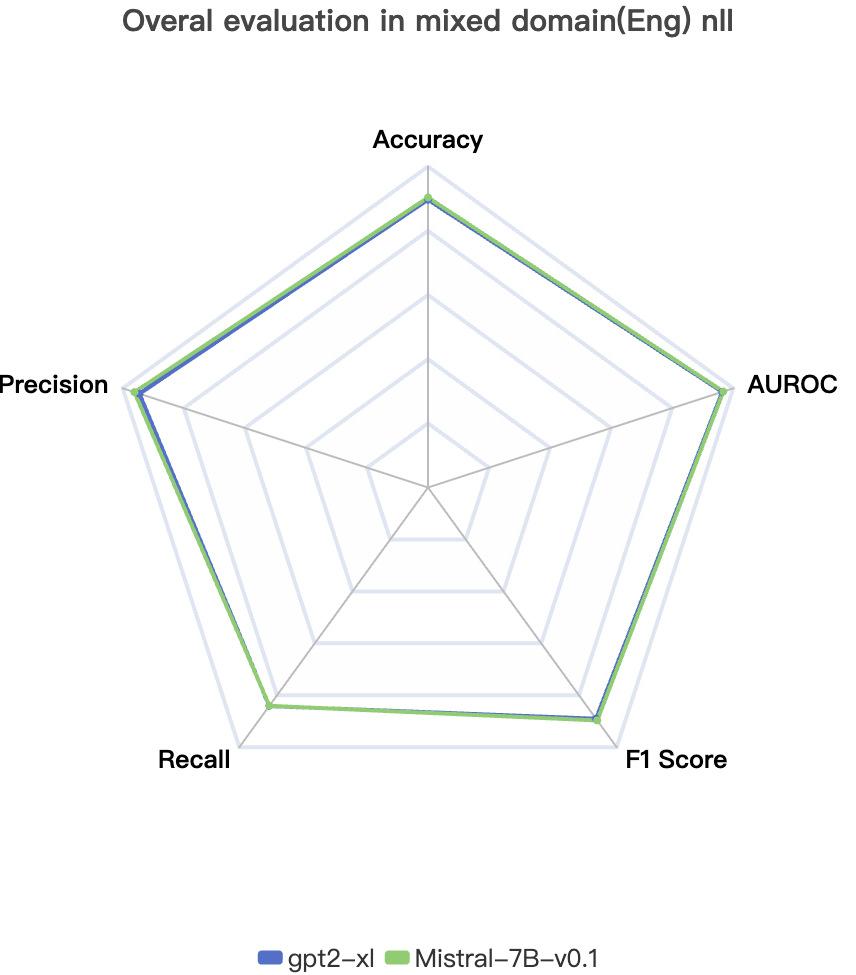
\includegraphics[width=0.5\linewidth]{images/Overal evaluation in mixed domain(Eng) nll.png}
        \label{fig:enter-label}
        \caption{Overal evaluation in mixed domain(Eng)}
    \end{figure}
   

\textbf{In the English mixed domain}, the metrics of the two models are almost identical.


 \begin{figure}[H]
        \centering
    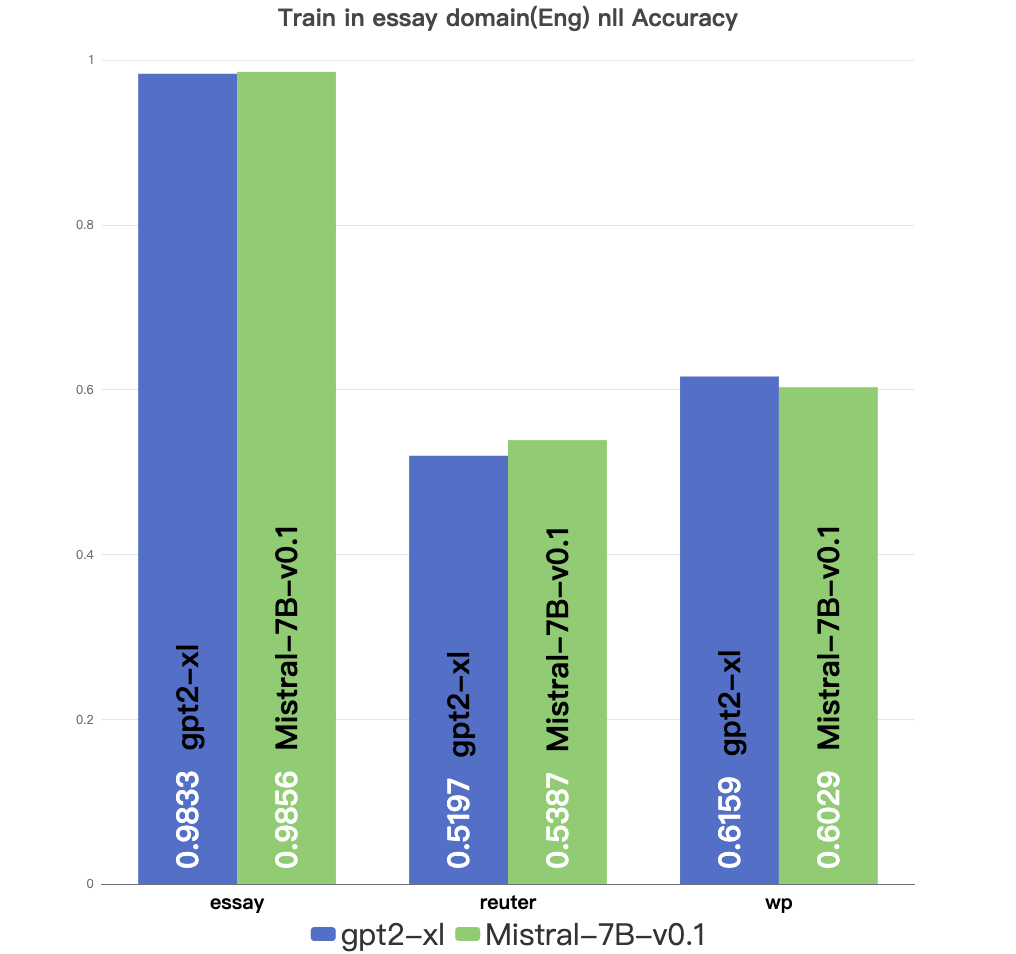
\includegraphics[width=0.8\linewidth]{images/Train in essay domain(Eng) nll Accuracy.png}
    \caption{Accuracy in essay domain(Eng)}
     \end{figure}
   

    \begin{figure}[H]
        \centering
    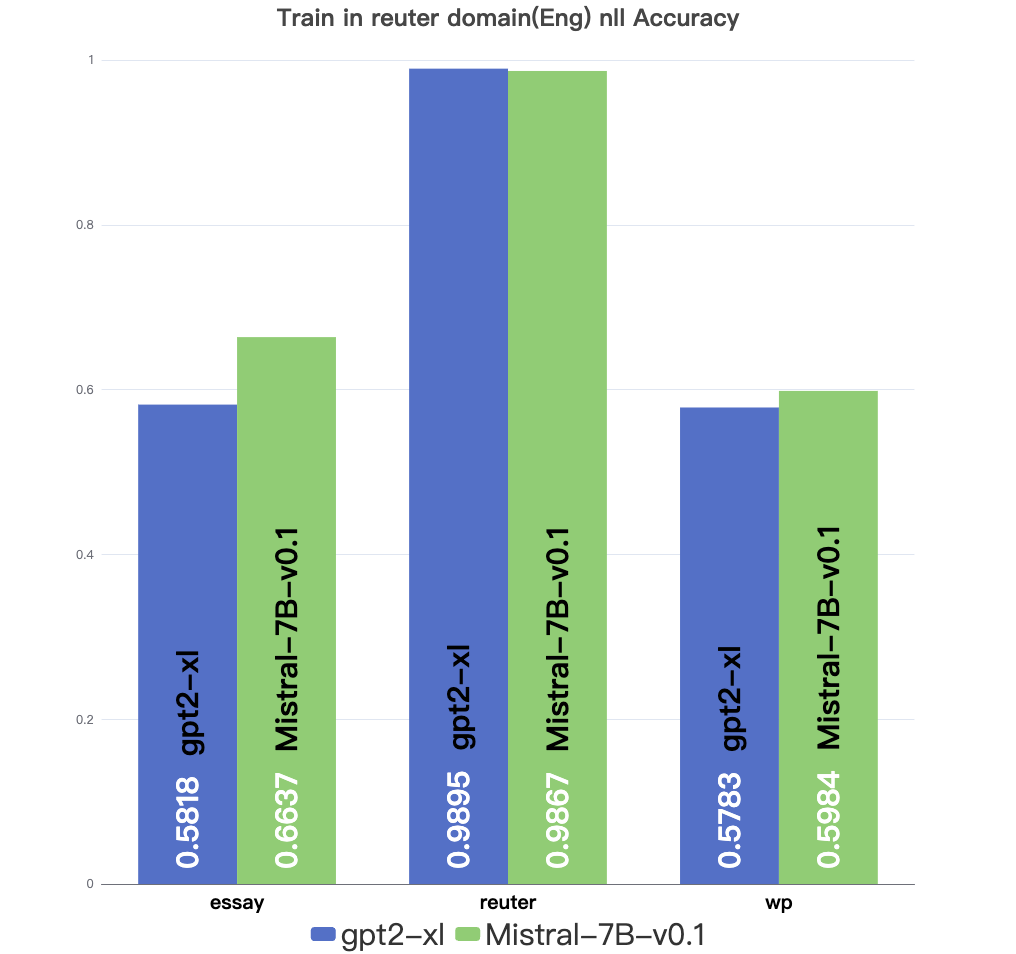
\includegraphics[width=0.8\linewidth]{images/Train in reuter domain(Eng) nll Accuracy.png}
    \caption{Accuracy in Reuter domain(Eng)}
\end{figure}
 
    \begin{figure}[H]
        \centering
    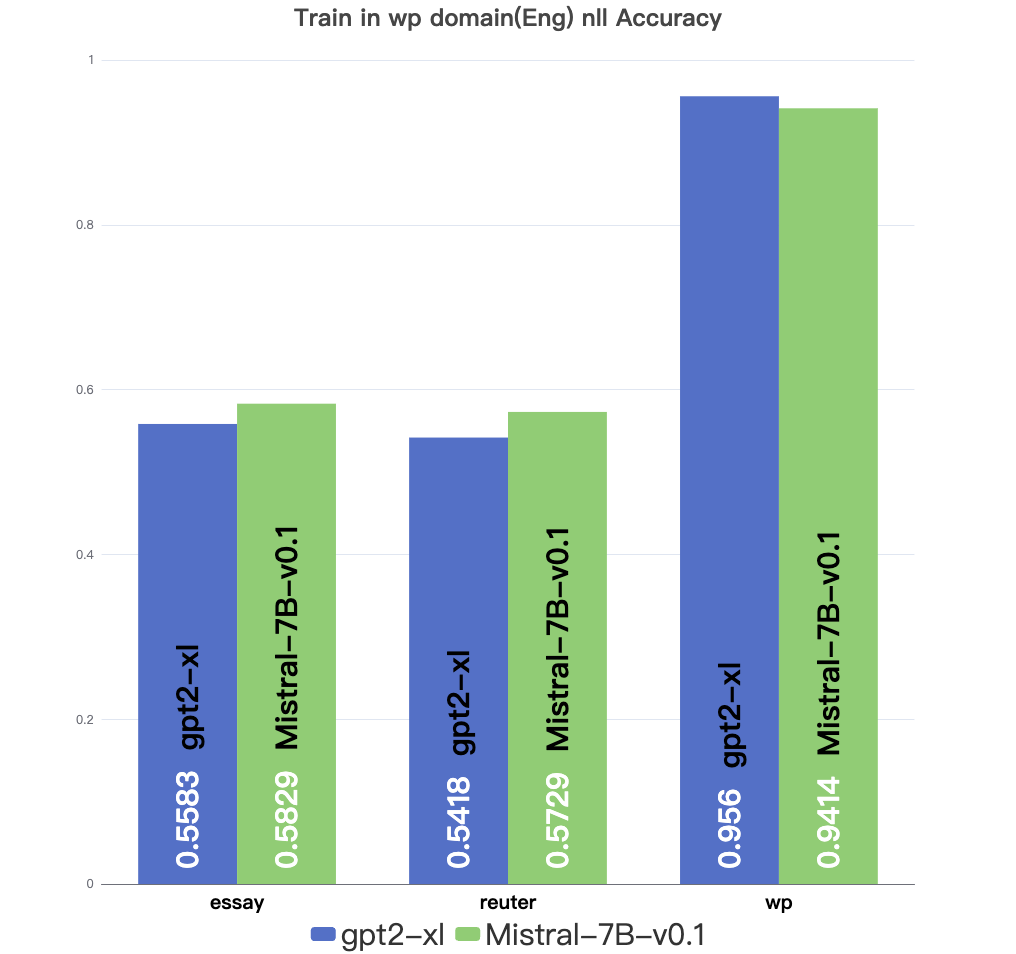
\includegraphics[width=0.8\linewidth]{images/Train in wp domain(Eng) nll Accuracy.png}
    \caption{Accuracy in wp domain(Eng)}
\end{figure}

For \textbf{out of domain test}, the models perform well within their \textbf{own training domain}, achieving accuracy \textbf{above 0.95}. However, accuracy significantly decreases when \textbf{tested on other domains}, often dropping \textbf{below 0.6}. Among the two models, \textbf{Mistral-7B-v0.1} demonstrates relatively better generalization across different domains.


\subsubsection{Chinese Dataset}

    \begin{figure}[H]
        \centering
        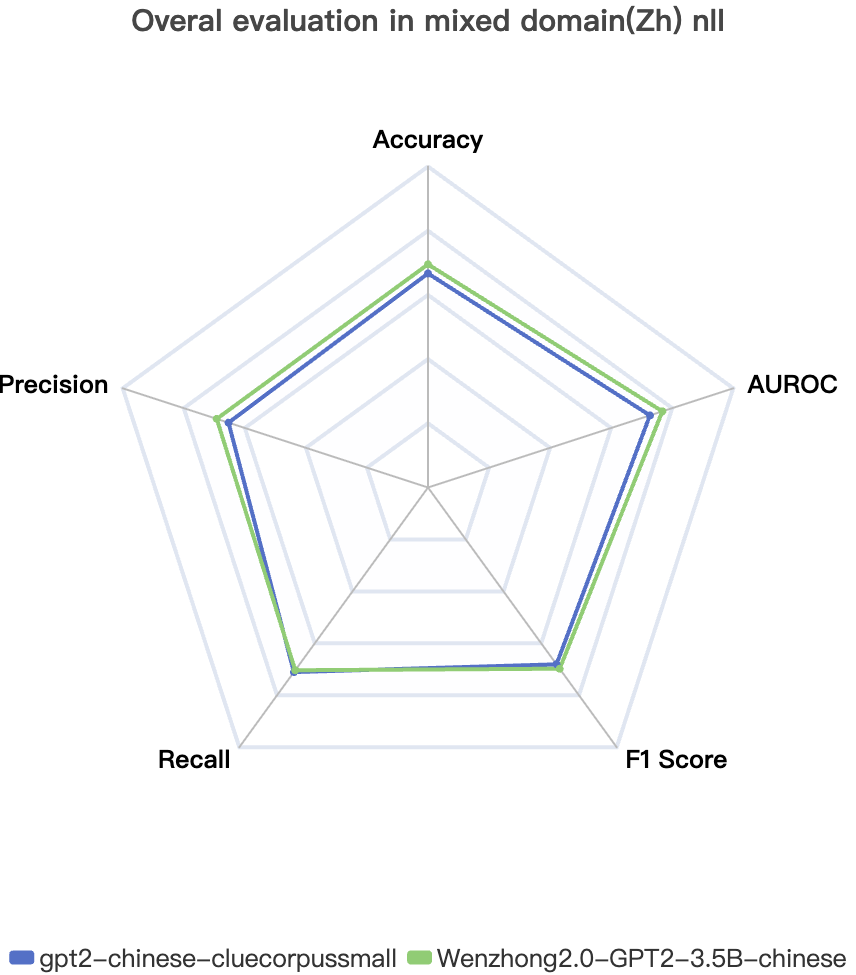
\includegraphics[width=0.6\linewidth]{images/Overal evaluation in mixed domain(Zh) nll.png}
        \label{fig:enter-label}
        \caption{Overal evaluation in mixed domain(Zh)}
    \end{figure}
  

\textbf{In the Chinese mixed domain,} \textbf{Wenzhong2.0-GPT2-3.5B-chinese} performs better across most metrics except recall.


     \begin{figure}[H]
        \centering
    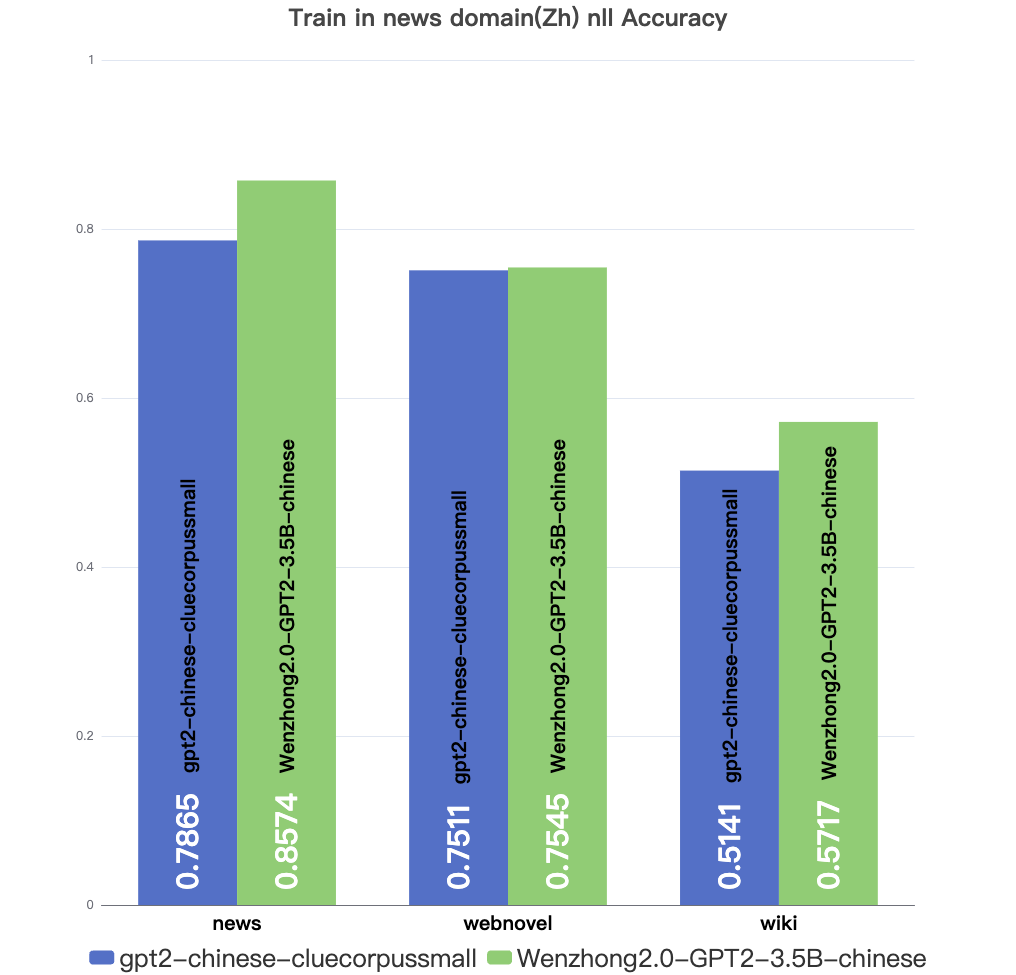
\includegraphics[width=0.6\linewidth]{images/Train in news domain(Zh) nll Accuracy.png}
    \caption{Accuracy in news domain(Zh)}
 \end{figure}
 
   \begin{figure}[H]
        \centering
    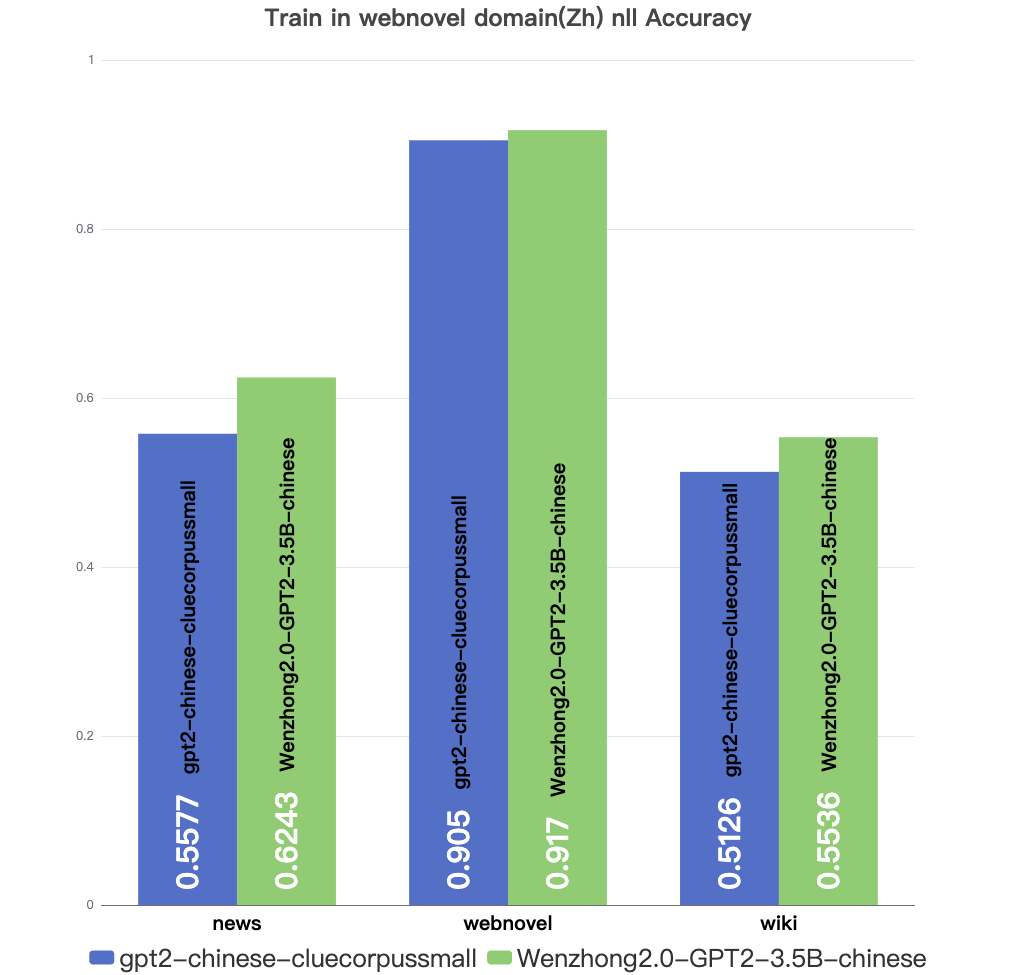
\includegraphics[width=0.8\linewidth]{images/Train in webnovel domain(Zh) nll Accuracy.png}
    \caption{Accuracy in Webnovel domain(Zh)}
\end{figure}
 
  \begin{figure}[H]
        \centering
    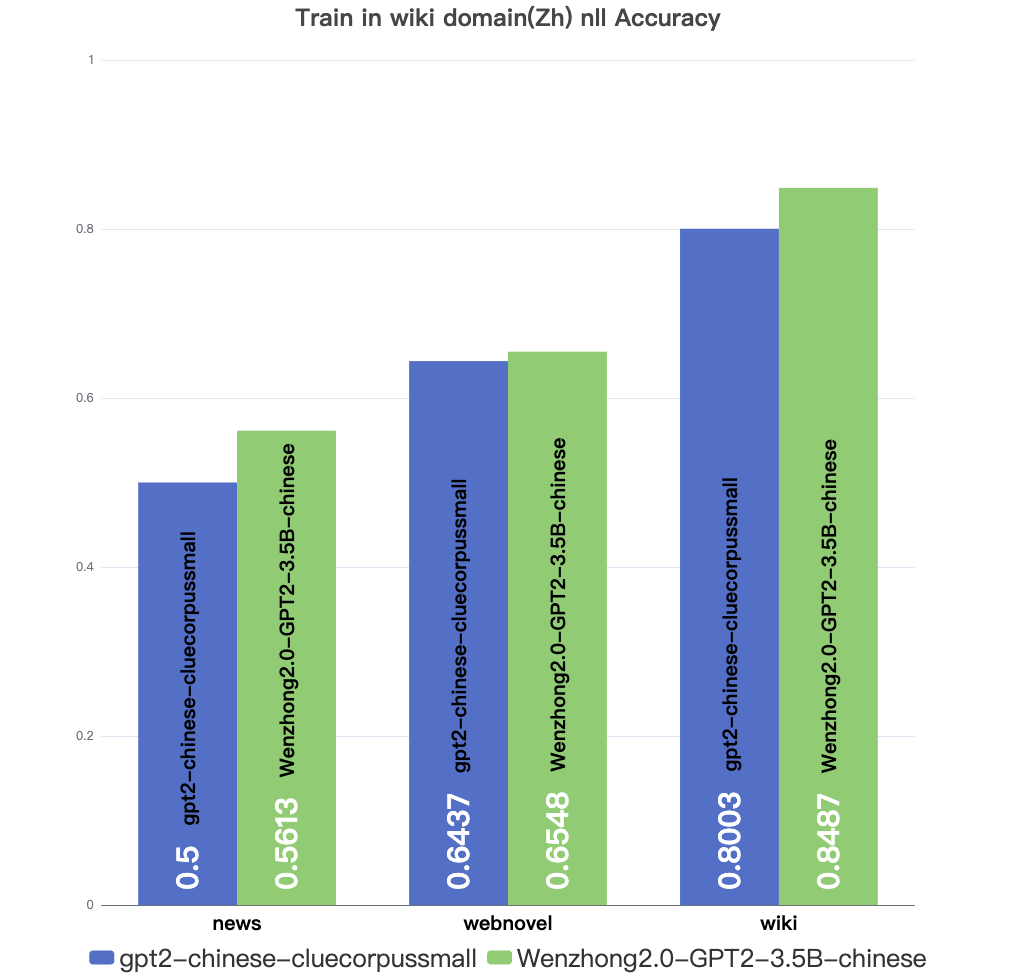
\includegraphics[width=0.8\linewidth]{images/Train in wiki domain(Zh) nll Accuracy.png}
    \caption{Accuracy in wiki domain(Zh)}
\end{figure}
For\textbf{ out of domain test}, the models perform well within their \textbf{own training domain}, achieving accuracy \textbf{above 0.8}. However, accuracy significantly decreases when \textbf{tested on other domains}, often dropping \textbf{below 0.6}. Among the two models, \textbf{Wenzhong2.0-GPT2-3.5B-chinese} exhibits relatively better generalization across different domains.


% --------------------------
\subsection{Zero-shot Detection}
We analyze the zero-shot detection performance using \textbf{aggregated power spectra across different datasets.}
\begin{figure}[H]
    \centering

    % 第一行
    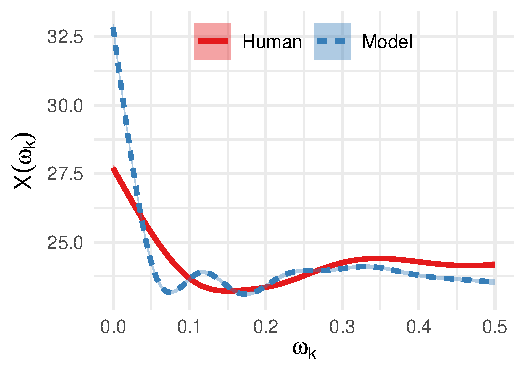
\includegraphics[width=0.3\linewidth]{images/en_essay_aggregated.pdf}
    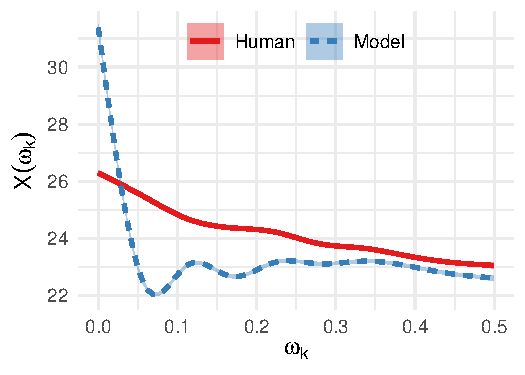
\includegraphics[width=0.3\linewidth]{images/en_reuter_aggregated.pdf}
    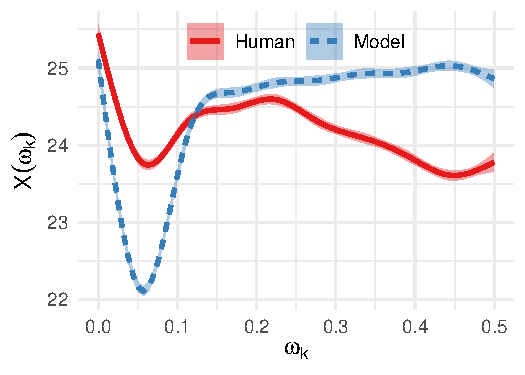
\includegraphics[width=0.3\linewidth]{images/eng_wp_aggregated.pdf}

    % 第一行文字说明
    \par\smallskip
    \makebox[0.5\linewidth]{\centering \textbf{k=5, model}}%
    \makebox[0.3\linewidth]{\centering \textbf{k=5, model}}%
    \makebox[0.3\linewidth]{\centering \textbf{k=3, model}}

    \par\vspace{0.6em}

    % 第二行
    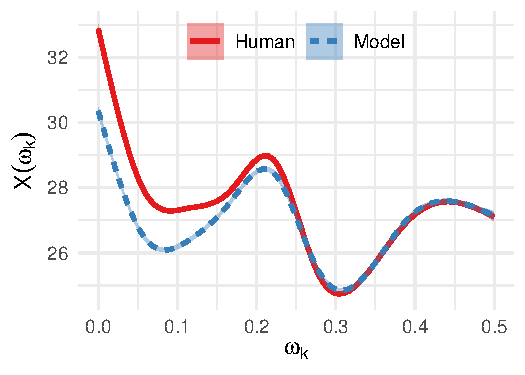
\includegraphics[width=0.3\linewidth]{images/zh_news_aggregated.pdf}
    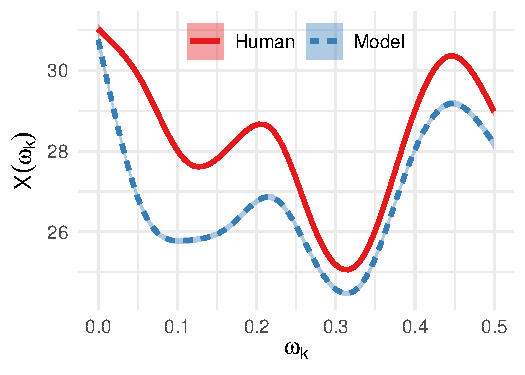
\includegraphics[width=0.3\linewidth]{images/zh_webnovel_aggregated.pdf}
    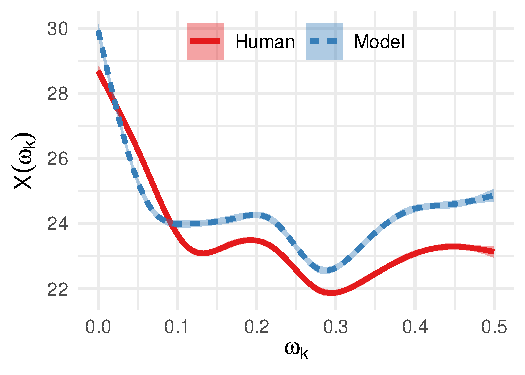
\includegraphics[width=0.3\linewidth]{images/zh_wiki_aggregated.pdf}

    % 第二行文字说明
    \par\smallskip
    \makebox[0.5\linewidth]{\centering \textbf{k=46, human}}%
    \makebox[0.3\linewidth]{\centering \textbf{k=50, human}}%
    \makebox[0.3\linewidth]{\centering \textbf{k=49, human}}

    \caption{Aggregated power spectra for zero-shot detection across different datasets.}
\end{figure}


For English texts, the model can distinguish between human-written and LLM-generated texts using only \textbf{a small number of low-frequency} features. Notably, for English texts, LLM-generated texts exhibit \textbf{higher} spectral power than human texts, whereas for Chinese texts, LLM-generated texts show \textbf{lower} spectral power.

\subsubsection{English Dataset}
    \begin{figure}[H]
        \centering
        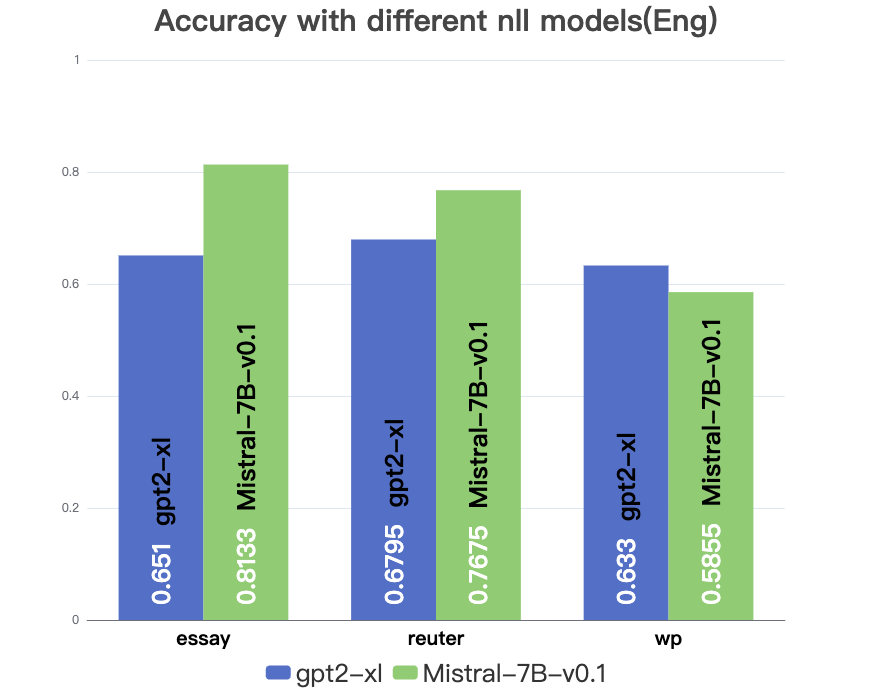
\includegraphics[width=0.8\linewidth]{images/Accuracy with different nll models(Eng).png}
        \label{fig:enter-label}
        \caption{Accuracy with different nll models(Eng)}
    \end{figure}
    
\textbf{Mistral-7B-v0.1} outperforms GPT2-XL in both the Essay and Reuter domains, achieving accuracy scores \textbf{above 0.75}. However, both models \textbf{struggle} on the wp domain, with accuracies of \textbf{0.63} and \textbf{0.59} respectively. Additionally, \textbf{Mistral-7B-v0.1} generates \textbf{better negative log-likelihood (NLL)} scores.



\begin{figure}[H]
    \centering
    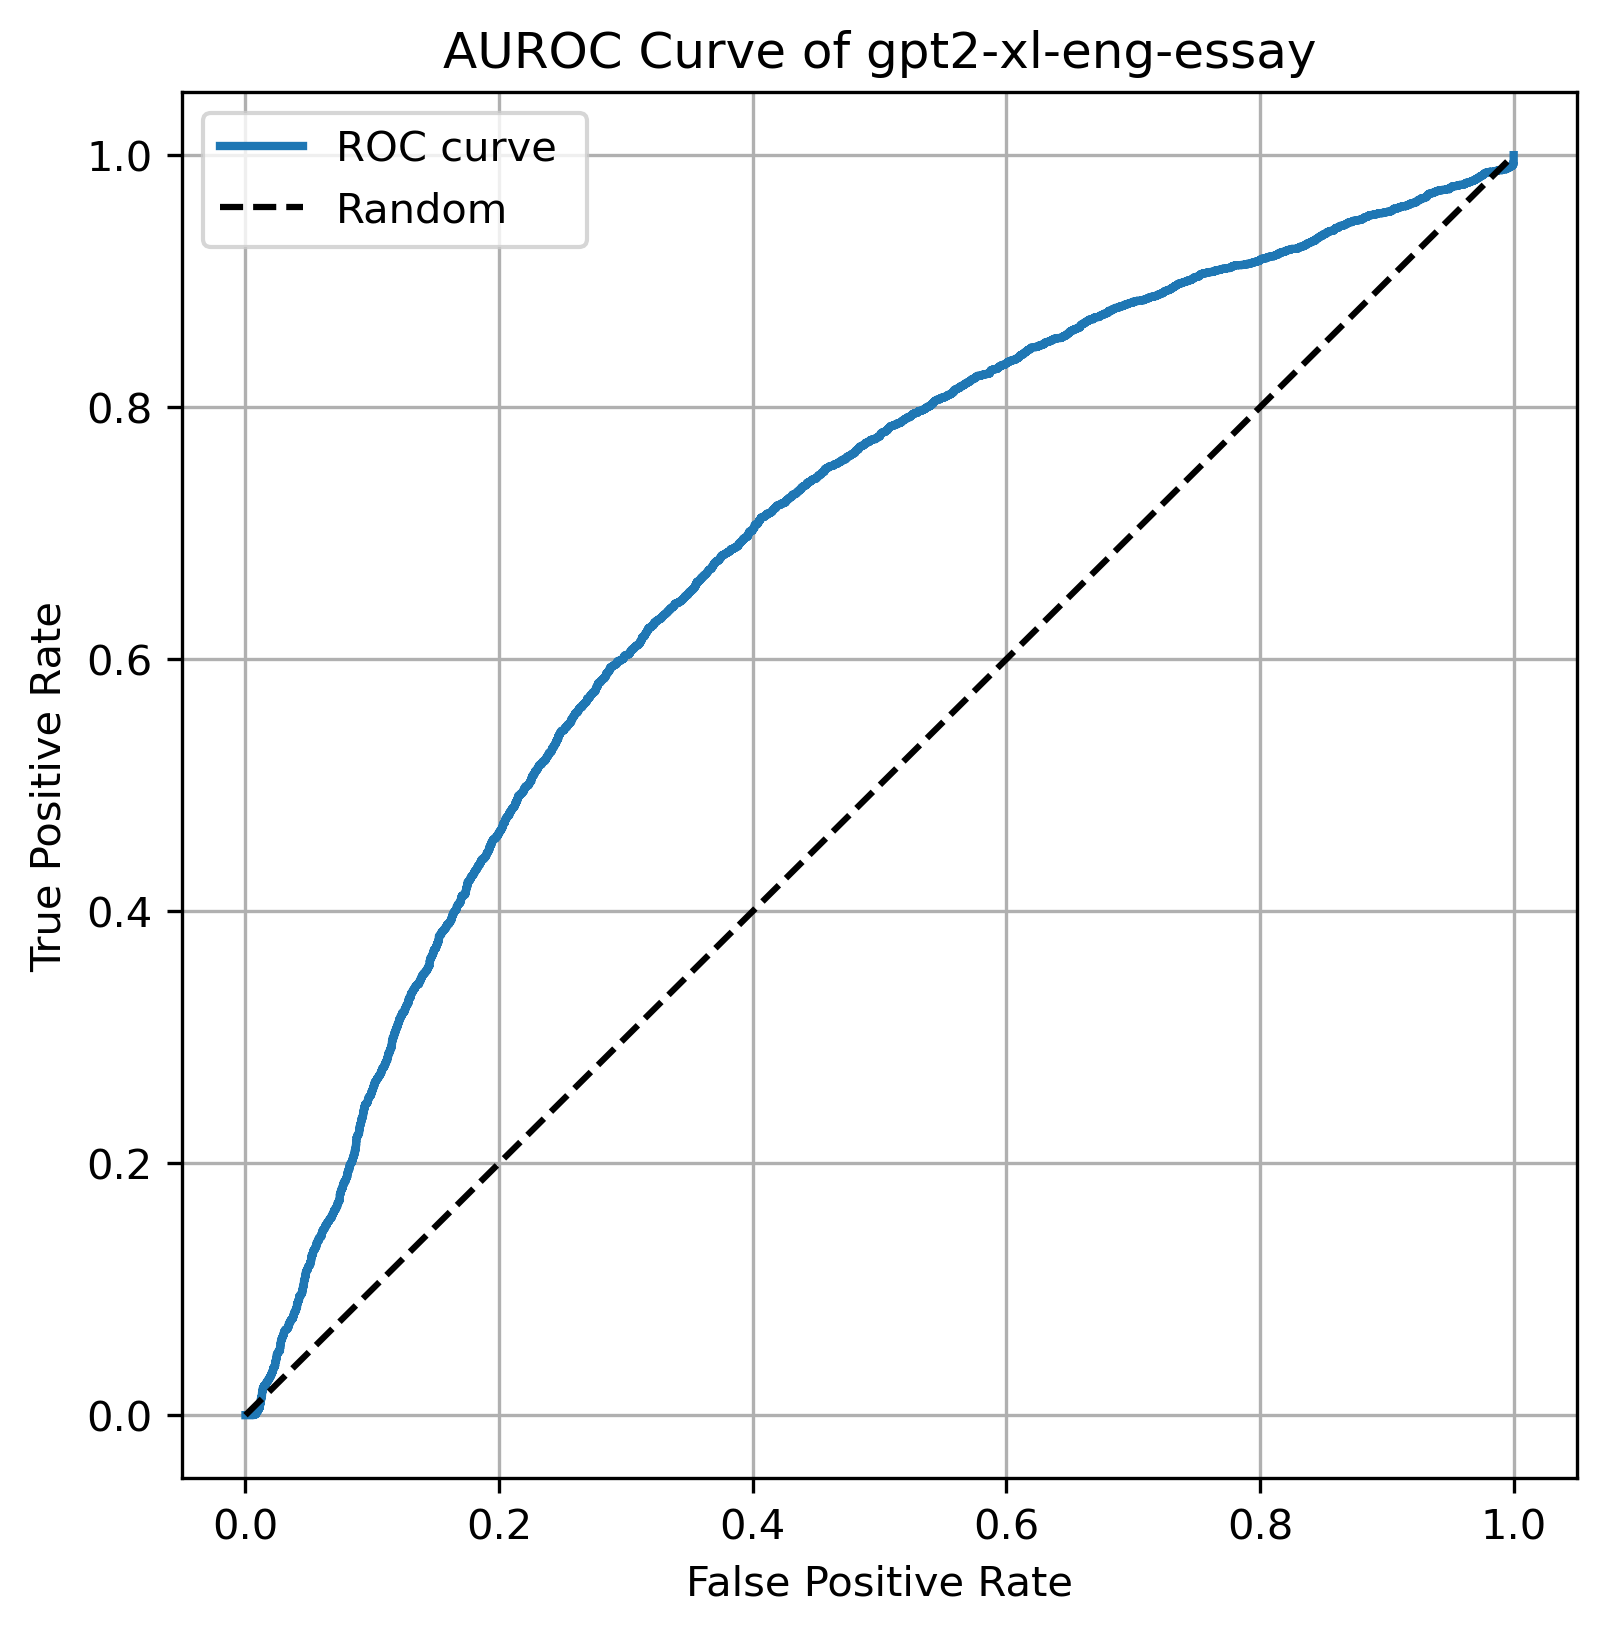
\includegraphics[width=0.3\linewidth]{images/gpt2-xl-eng-essay.png}
    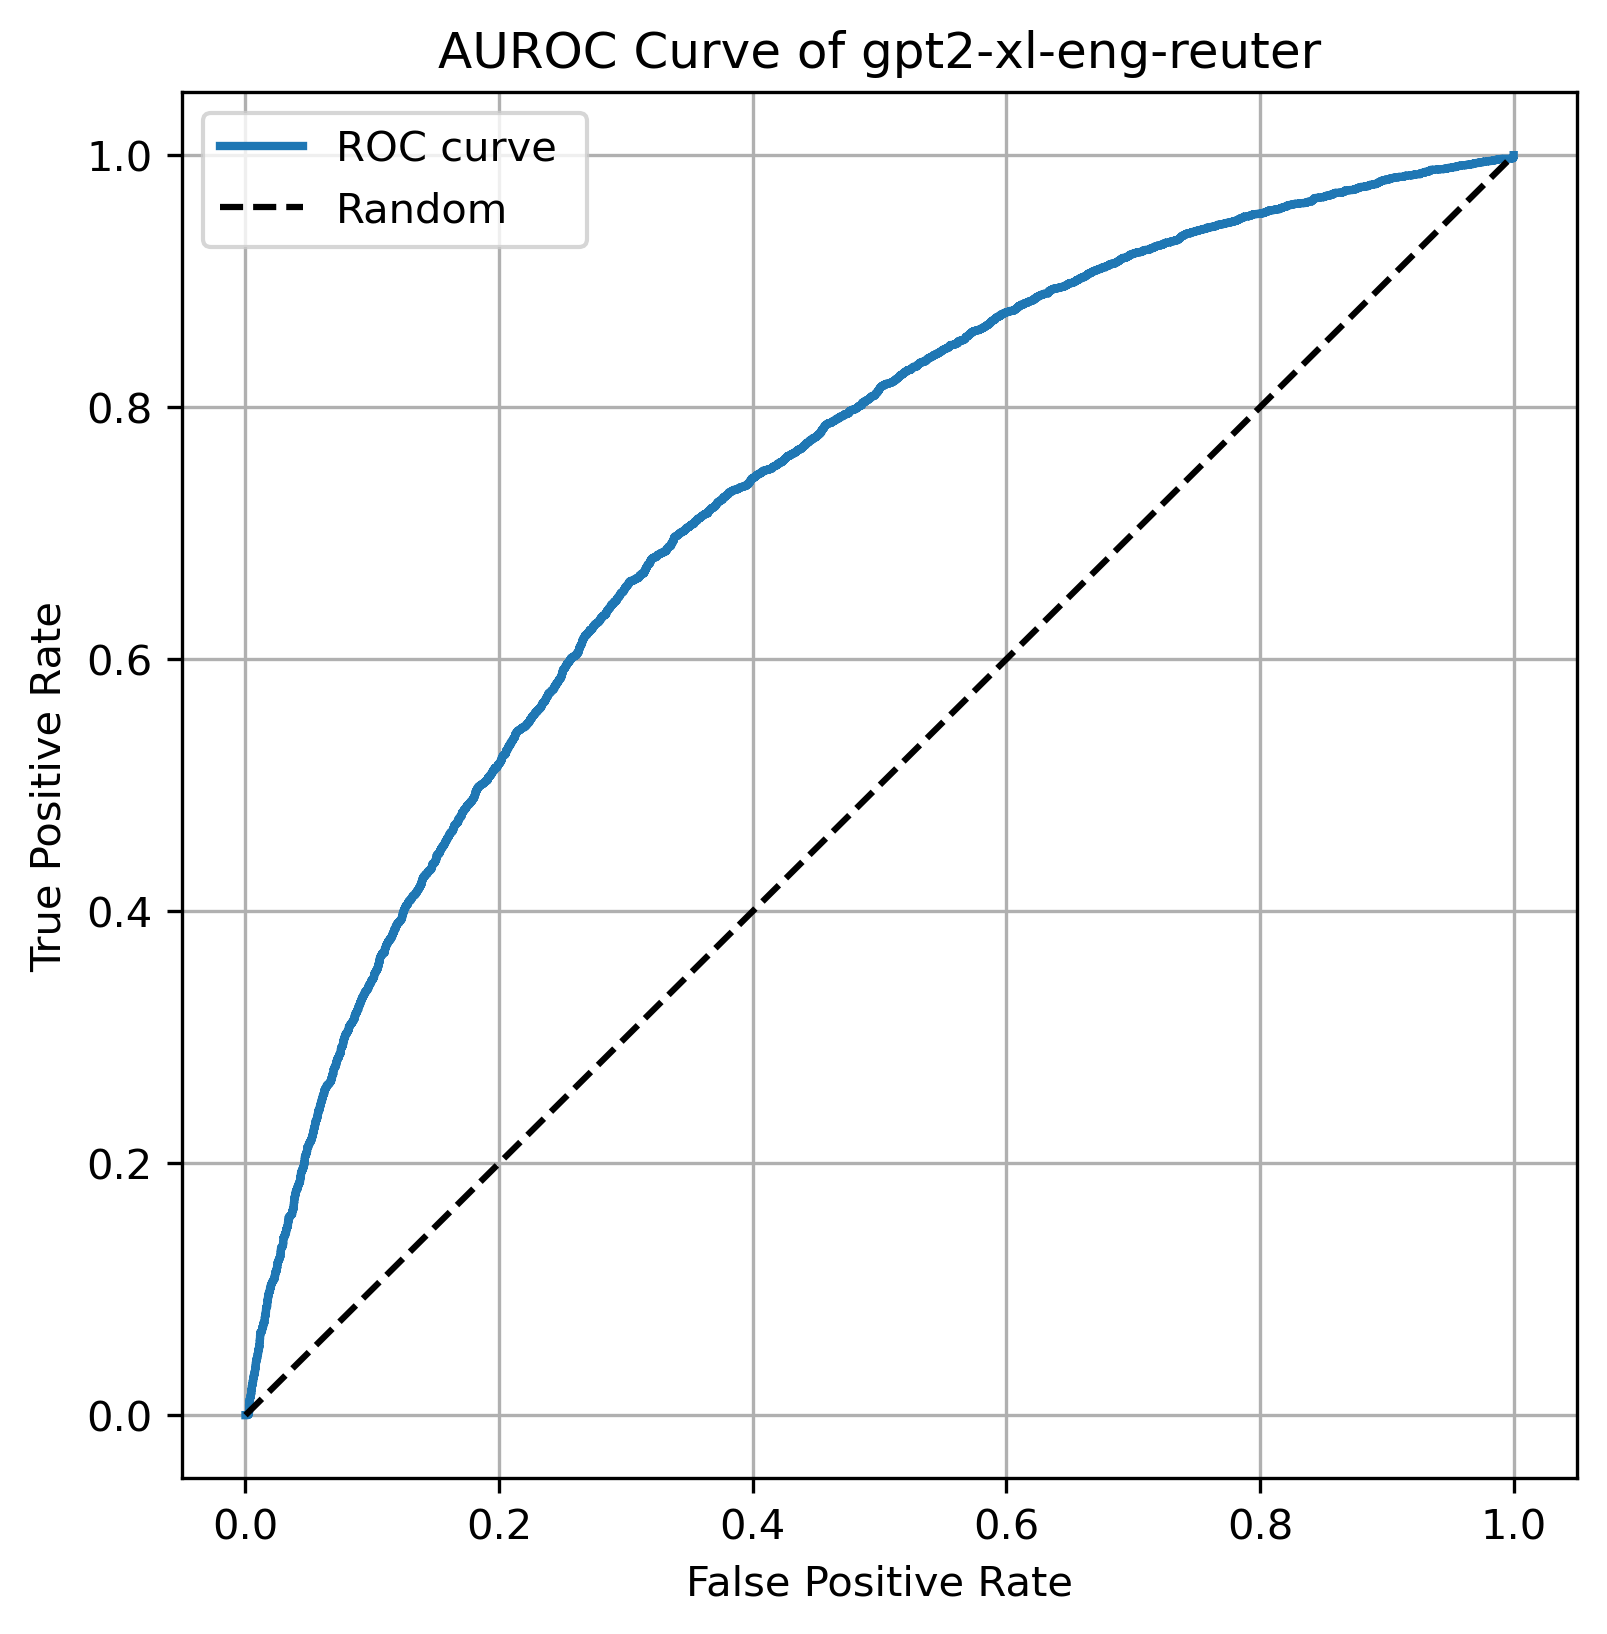
\includegraphics[width=0.3\linewidth]{images/gpt2-xl-eng-reuter.png}
    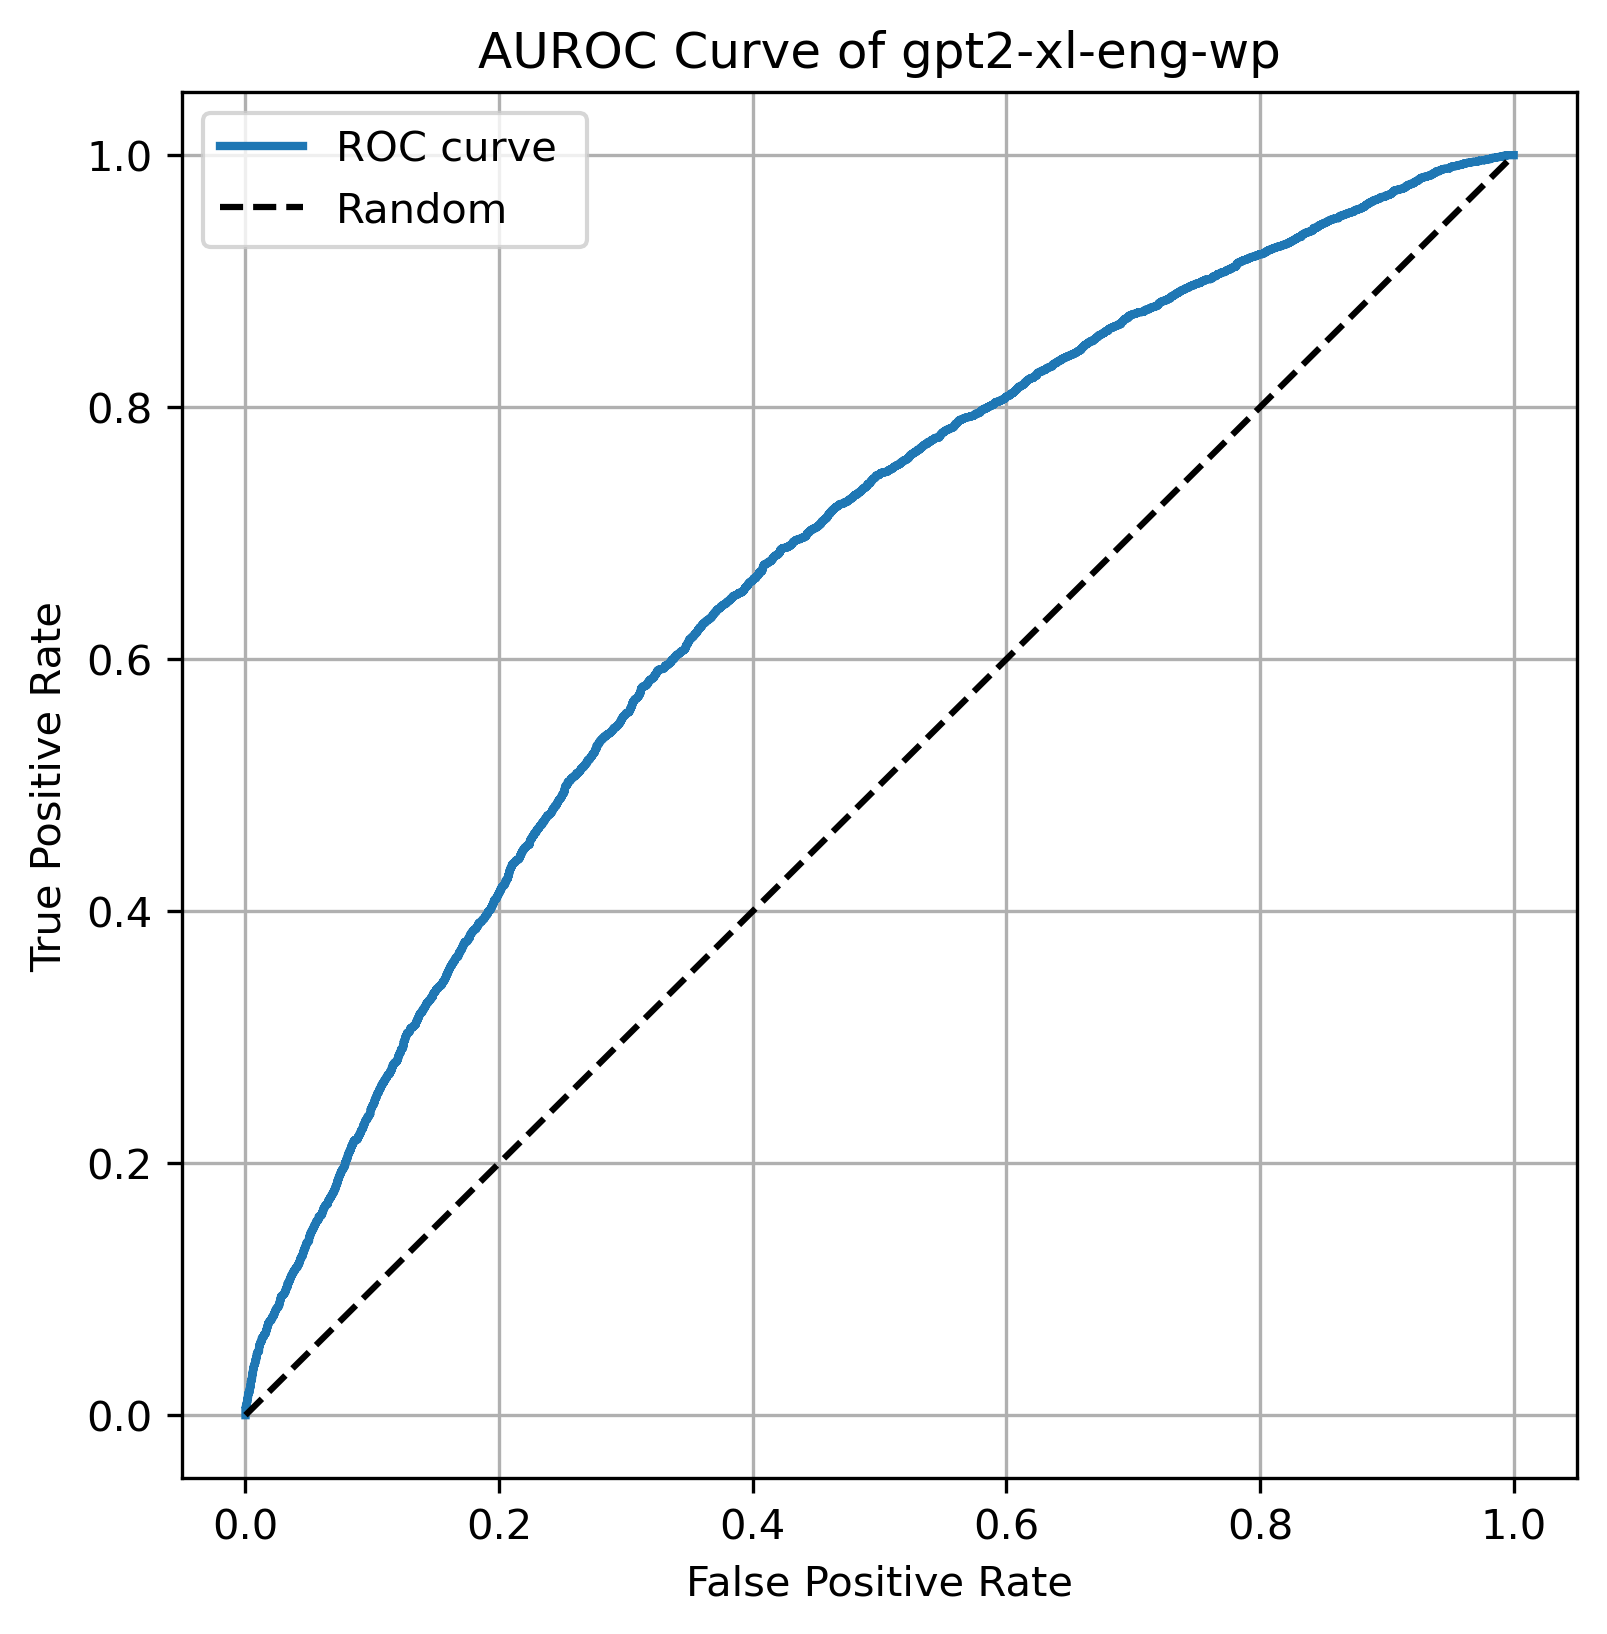
\includegraphics[width=0.3\linewidth]{images/gpt2-xl-eng-wp.png}
    
    \vspace{0.3cm}
    
    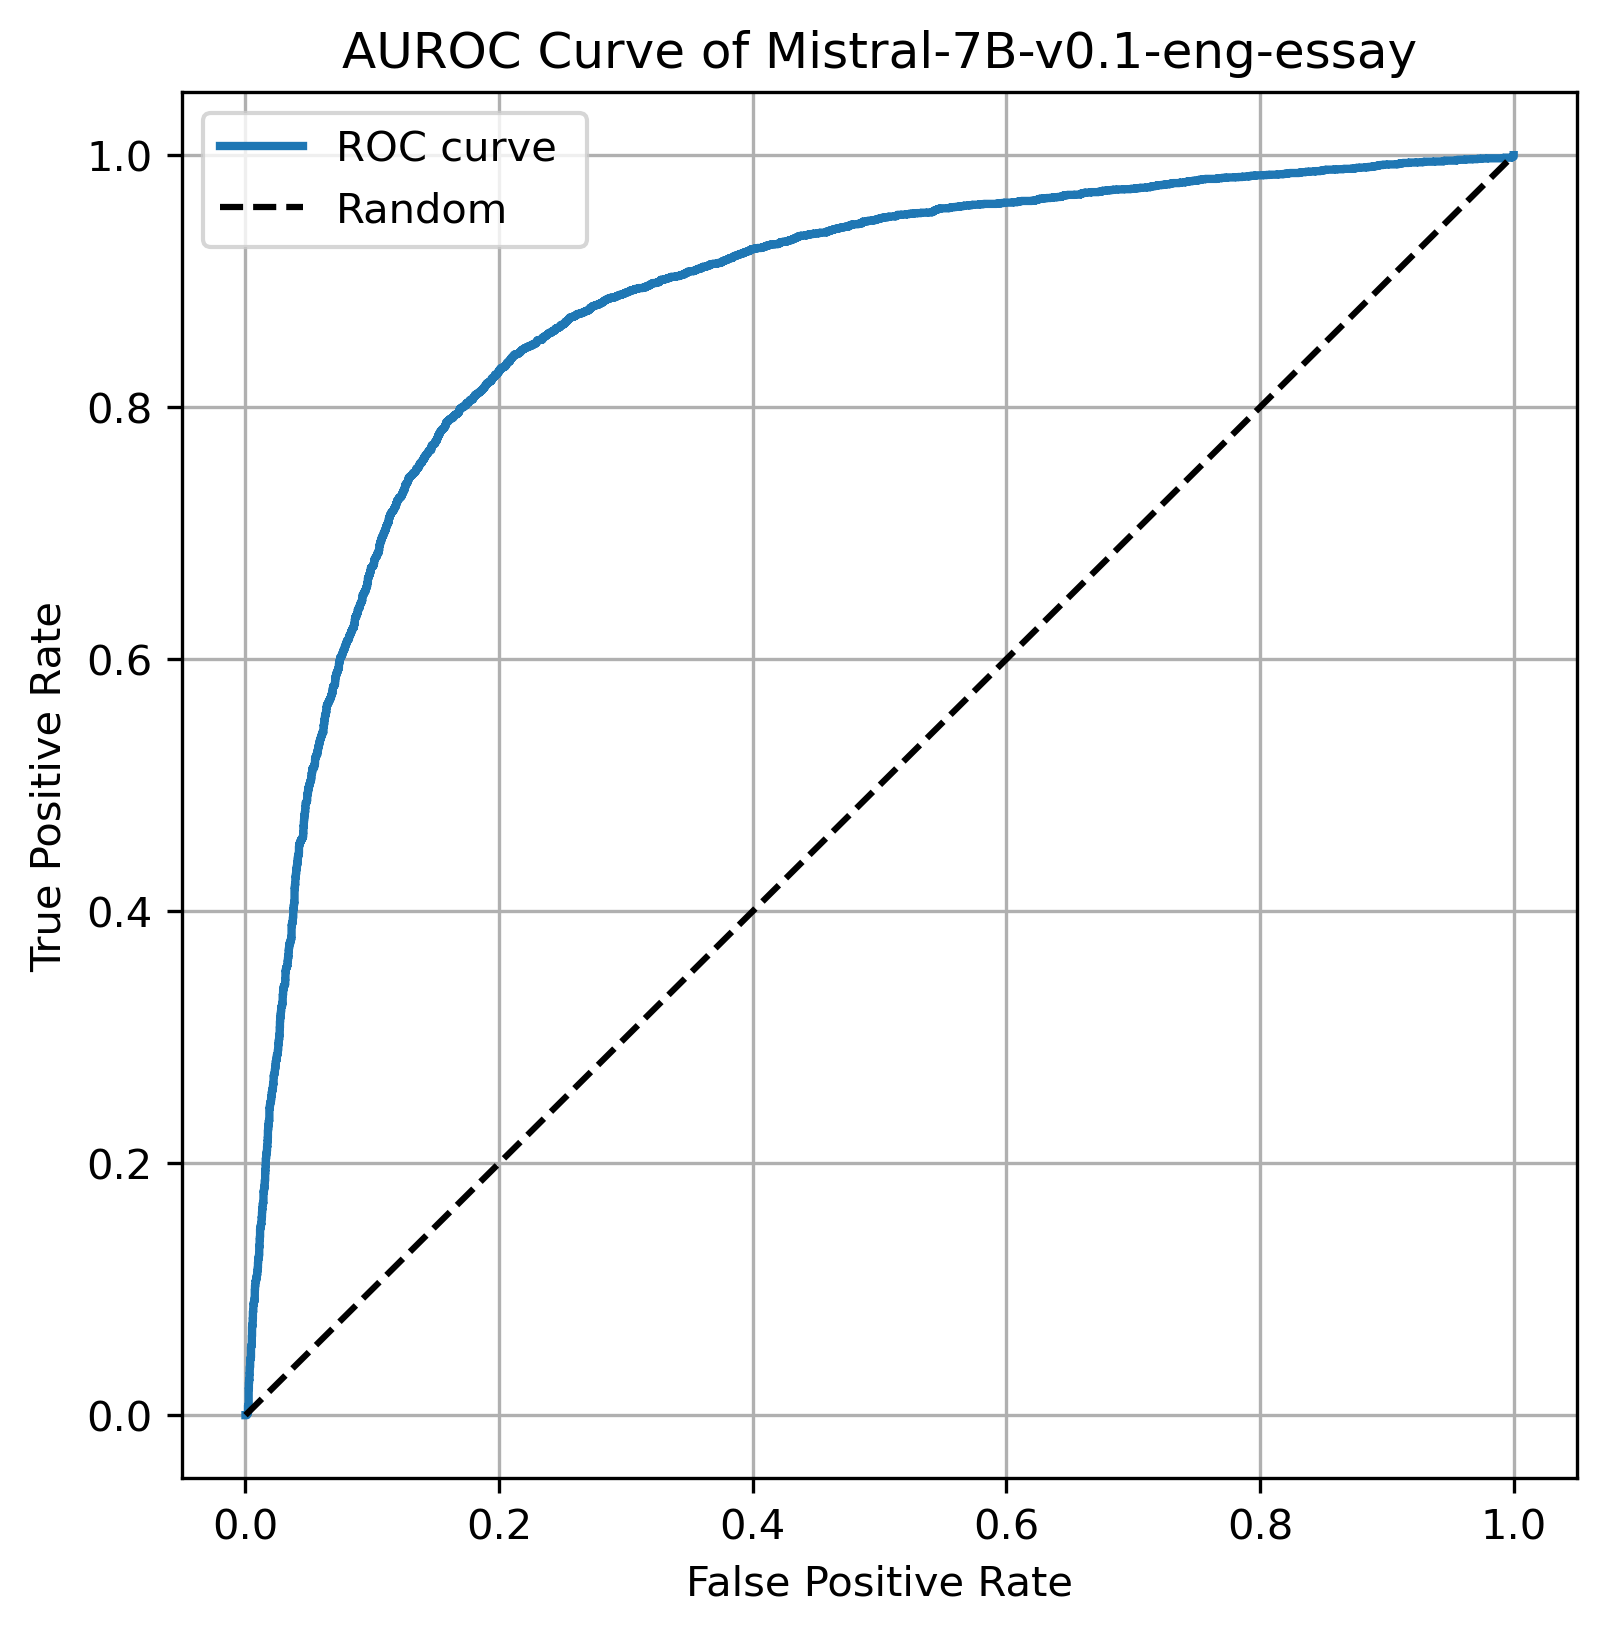
\includegraphics[width=0.3\linewidth]{images/Mistral-7B-v0.1-eng-essay.png}
    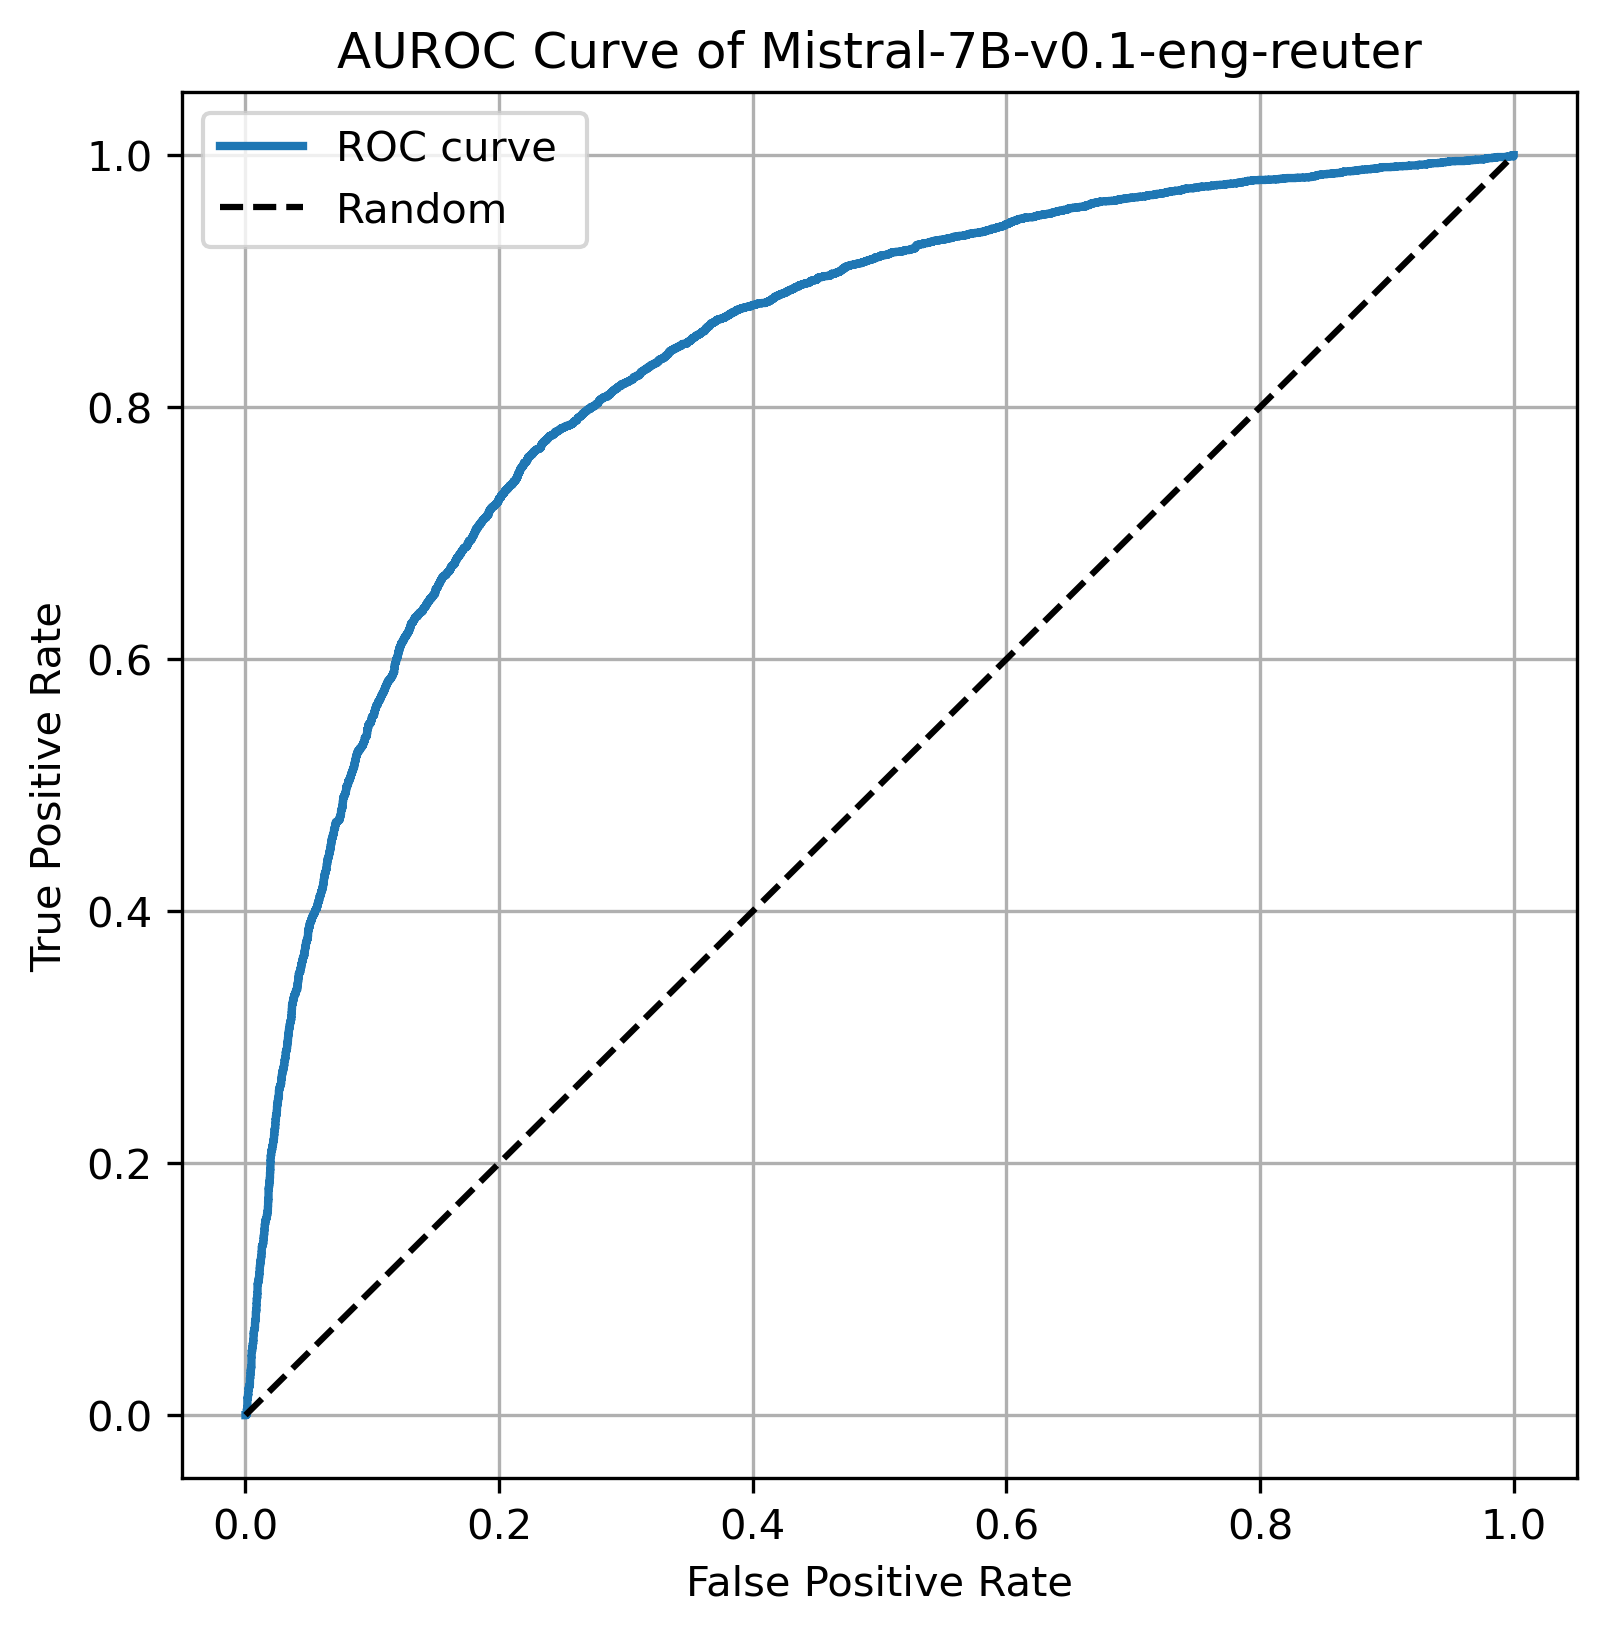
\includegraphics[width=0.3\linewidth]{images/Mistral-7B-v0.1-eng-reuter.png}
    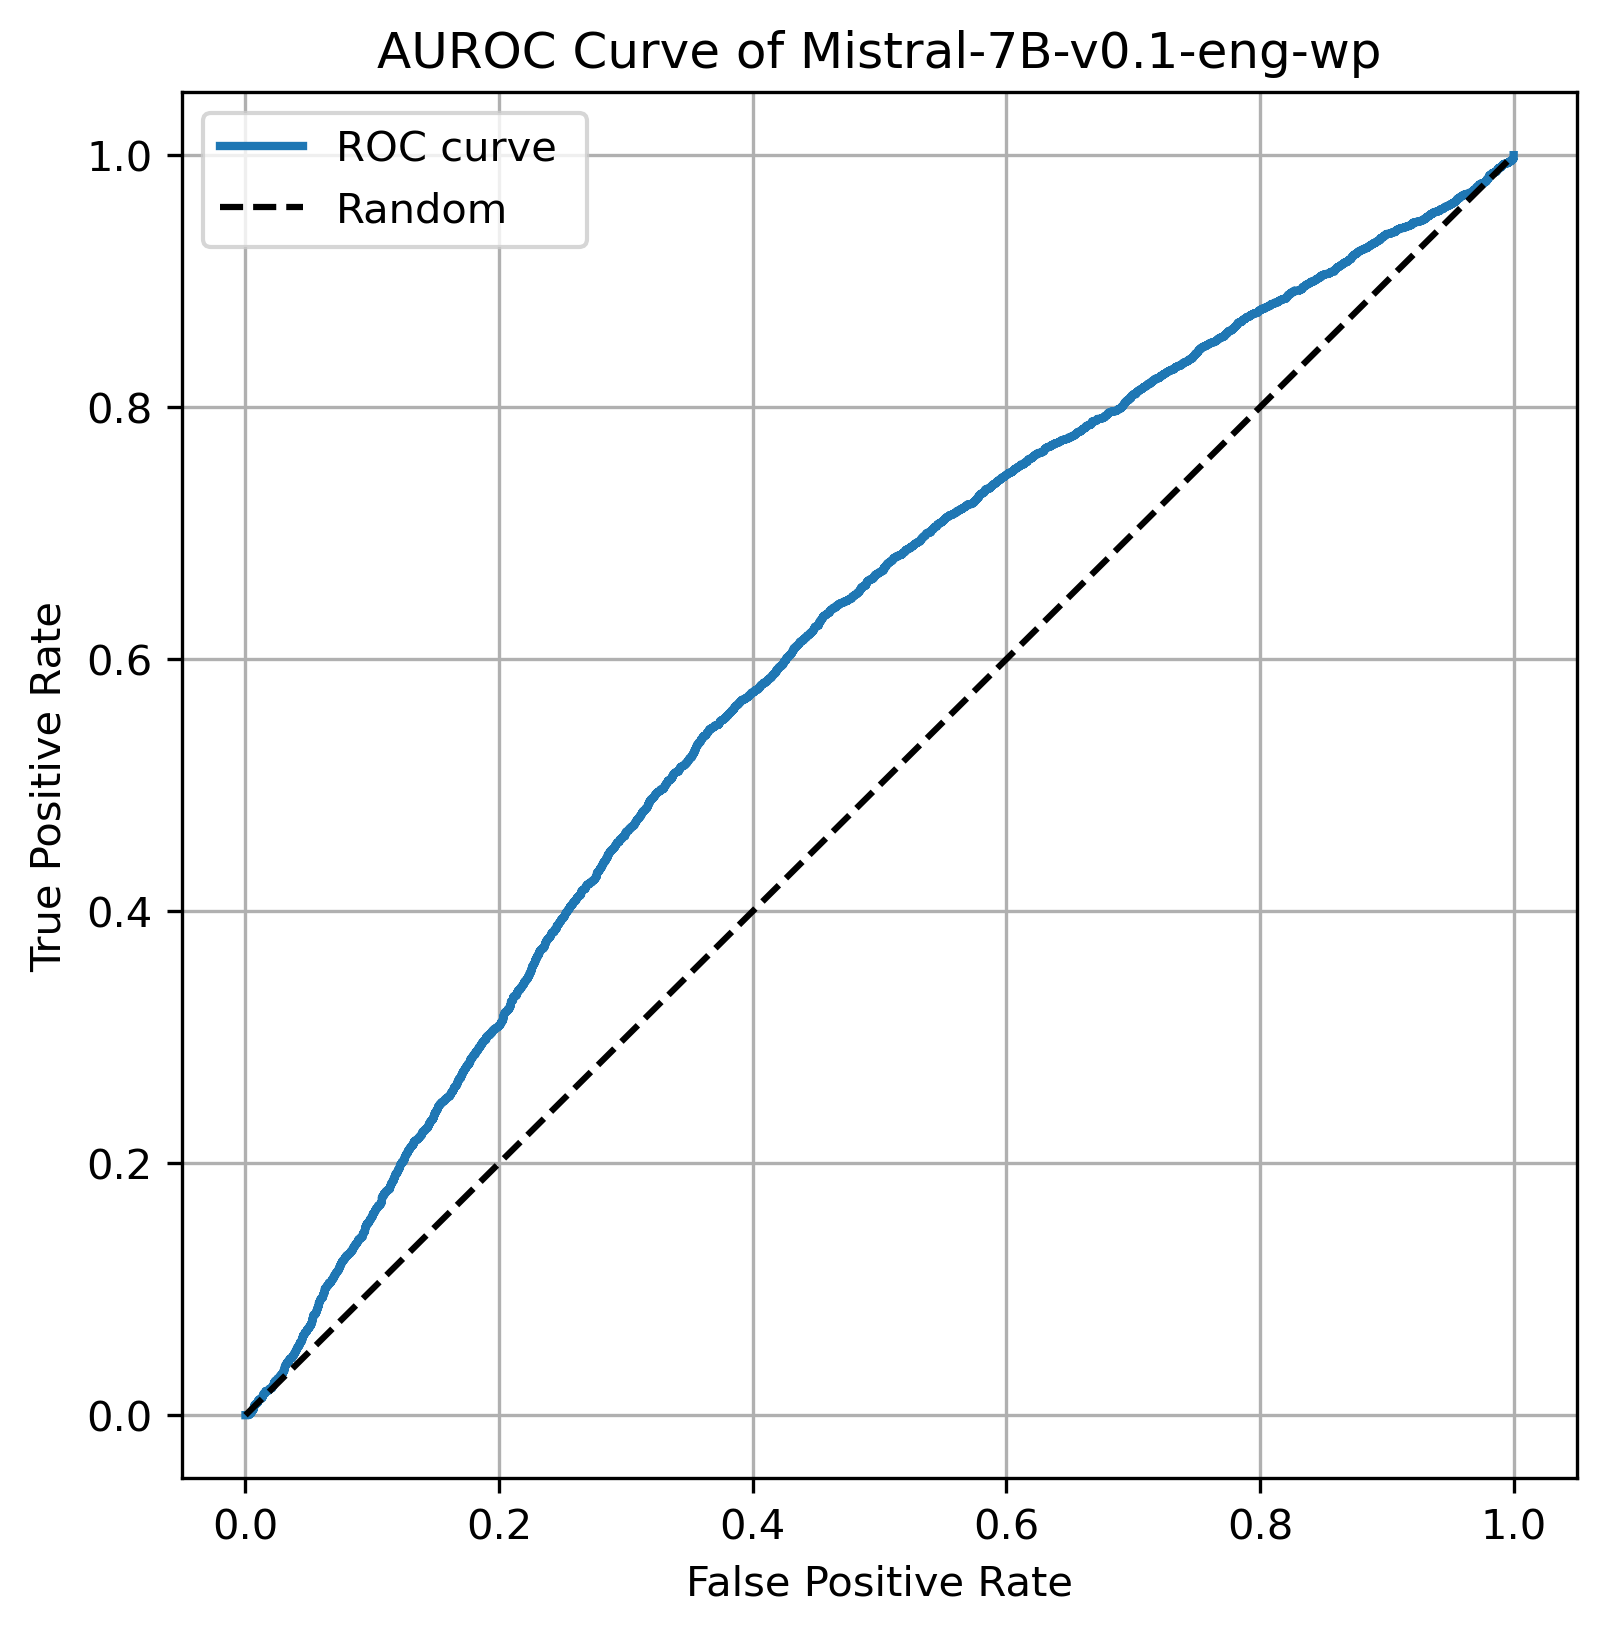
\includegraphics[width=0.3\linewidth]{images/Mistral-7B-v0.1-eng-wp.png}
    
    \caption{AUROC curves of GPT2-XL and Mistral-7B-v0.1 across English essay, reuter, and wp domains.}
\end{figure}

The ROC curves for \textbf{Mistral-7B-v0.1} on the essay and reuter datasets are closer to the top-left corner, indicating a stronger ability to distinguish between positive and negative samples. Conversely, the ROC curves on the \textbf{wp} dataset approach the diagonal line, suggesting performance close to random guessing and highlighting the increased difficulty in classification within this domain.

In the Zero-shot detection method, we compare model performance across English datasets using multiple evaluation metrics.
\begin{table}[H]
 \centering
    \caption{gpt2-xl-Eng}
    \label{tab:my_label}
\setlength{\tabcolsep}{2pt}
\renewcommand{\arraystretch}{1.0}
\vspace{0.3cm}
\resizebox{0.4\textwidth}{!}{%
\begin{tabular}{|l|c|c|c|}
\hline
\textbf{FT domain} & \textbf{essay} & \textbf{reuter} & \textbf{wp} \\
\hline
Accuracy & 0.6510 & 0.6795 & 0.6330 \\
\hline
AUROC & 0.6899 & 0.7348 & 0.6732 \\
\hline
\end{tabular}%
}
\end{table}

\begin{table}[H]
 \centering
    \caption{Mistral-7B-v0.1-Eng}
    \label{tab:my_label}
\setlength{\tabcolsep}{2pt}
\renewcommand{\arraystretch}{1.0}
\vspace{0.3cm}
\resizebox{0.4\textwidth}{!}{%
\begin{tabular}{|l|c|c|c|}
\hline
\textbf{FT domain} & \textbf{essay} & \textbf{reuter} & \textbf{wp} \\
\hline
Accuracy & 0.8133 & 0.7675 & 0.5855 \\
\hline
AUROC & 0.8798 & 0.8375 & 0.6044 \\
\hline
\end{tabular}%
}
\end{table}



\subsubsection{Chinese Dataset}


    \begin{figure}[h!]
        \centering
        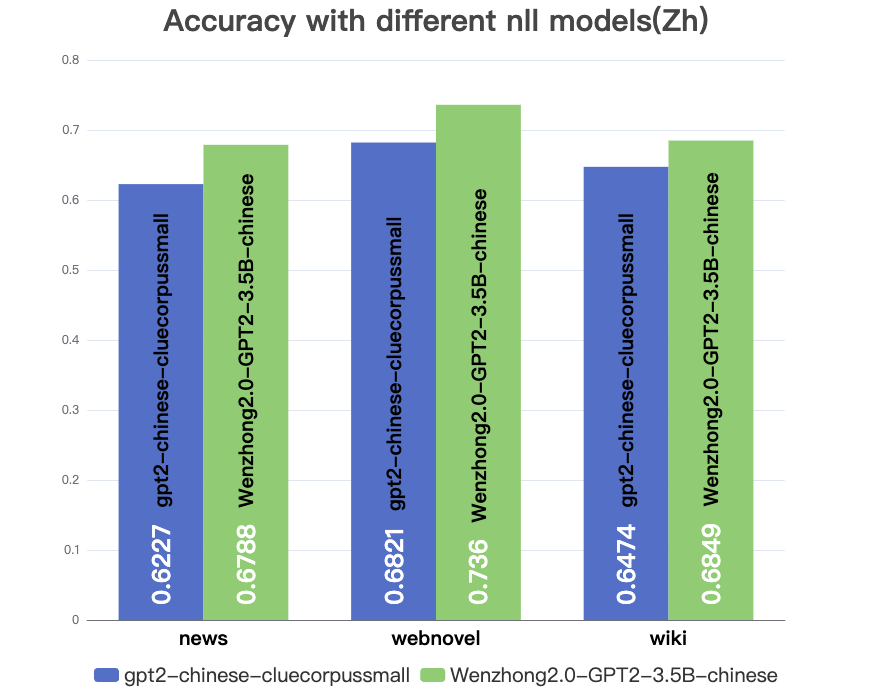
\includegraphics[width=0.75\linewidth]{images/Accuracy with different nll models(Zh).png}
        \label{fig:enter-label}
        \caption{Accuracy with different nll models(Zh)}
    \end{figure}
    
\textbf{Wenzhong2.0-GPT2-3.5B} consistently outperforms \textbf{gpt2-chinese-cluecorpussmall} across all evaluated domains. Both models achieve their highest accuracy and AUROC in the \textbf{webnovel} domain (0.73 and 0.82, respectively), while detecting differences in \textbf{news} texts proves more challenging, with corresponding scores of 0.64 and 0.68.


\begin{figure}[h!]
    \centering
    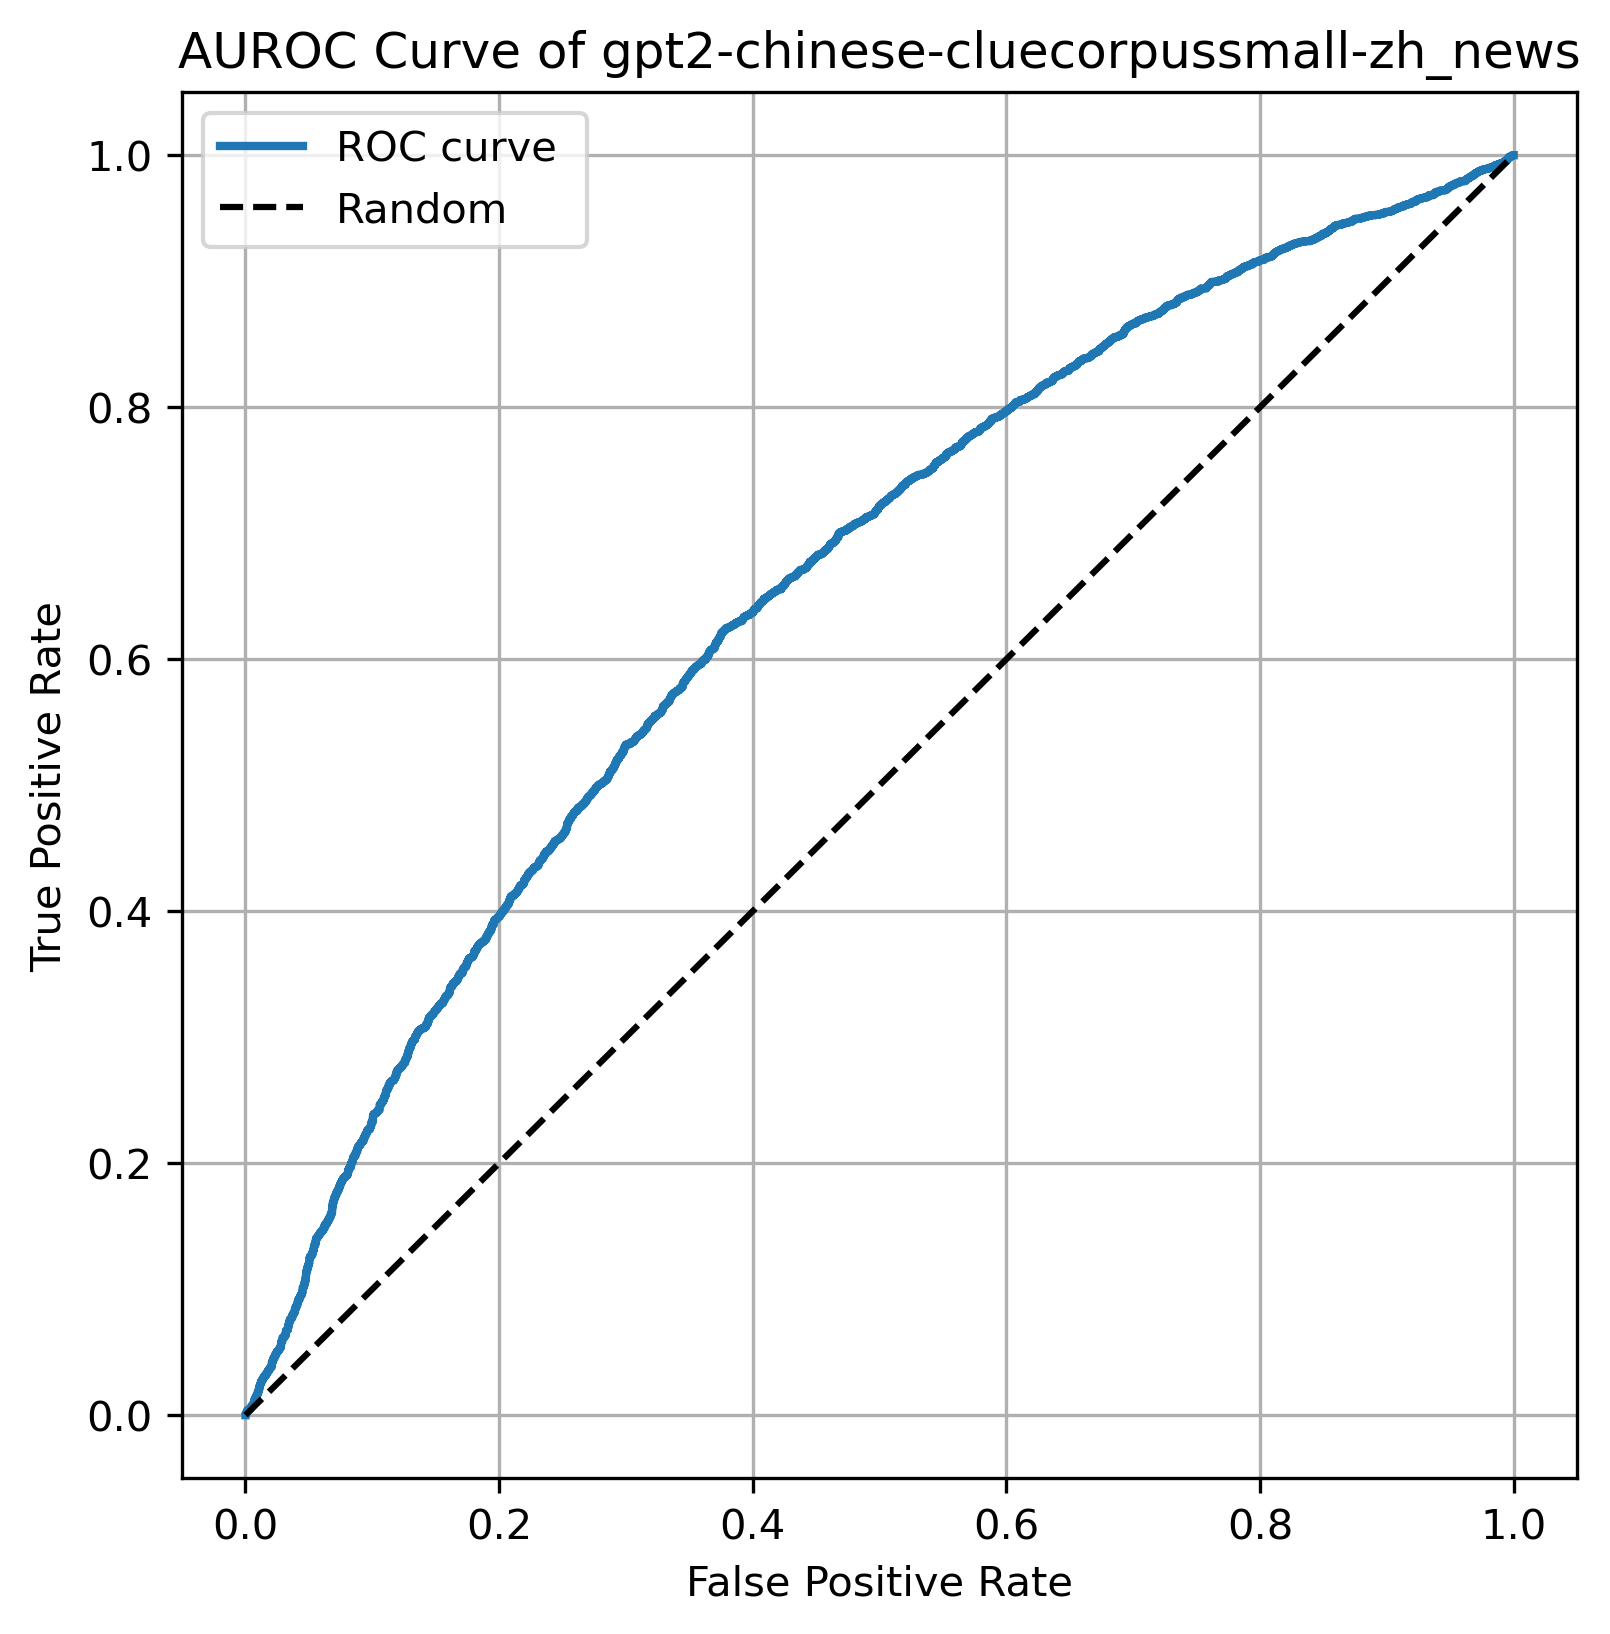
\includegraphics[width=0.3\linewidth]{images/gpt2-chinese-cluecorpussmall-zh_news.png}
    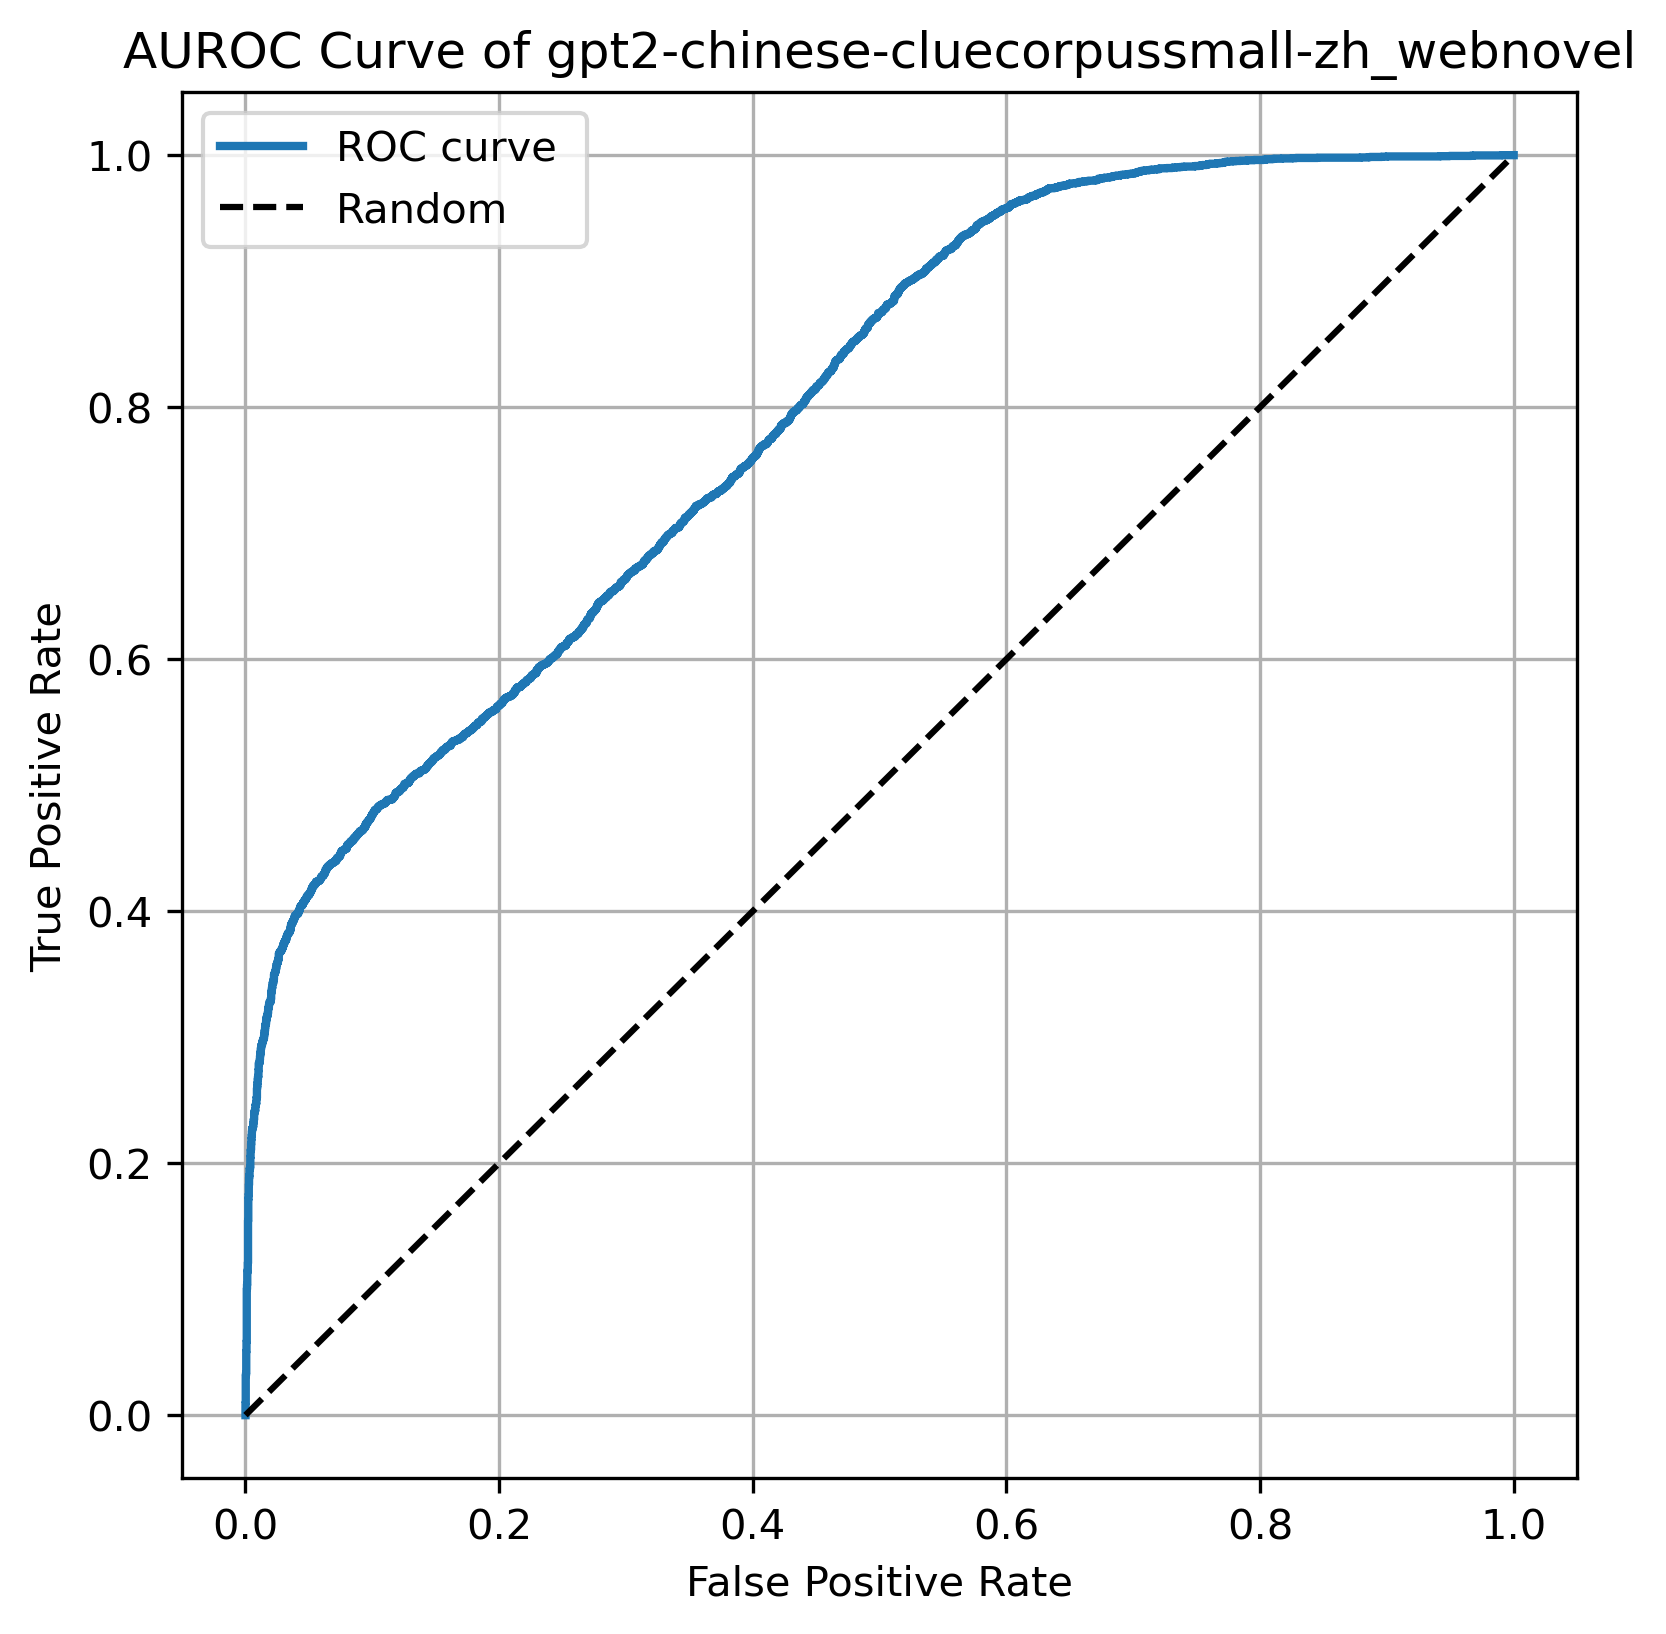
\includegraphics[width=0.3\linewidth]{images/gpt2-chinese-cluecorpussmall-zh_webnovel.png}
    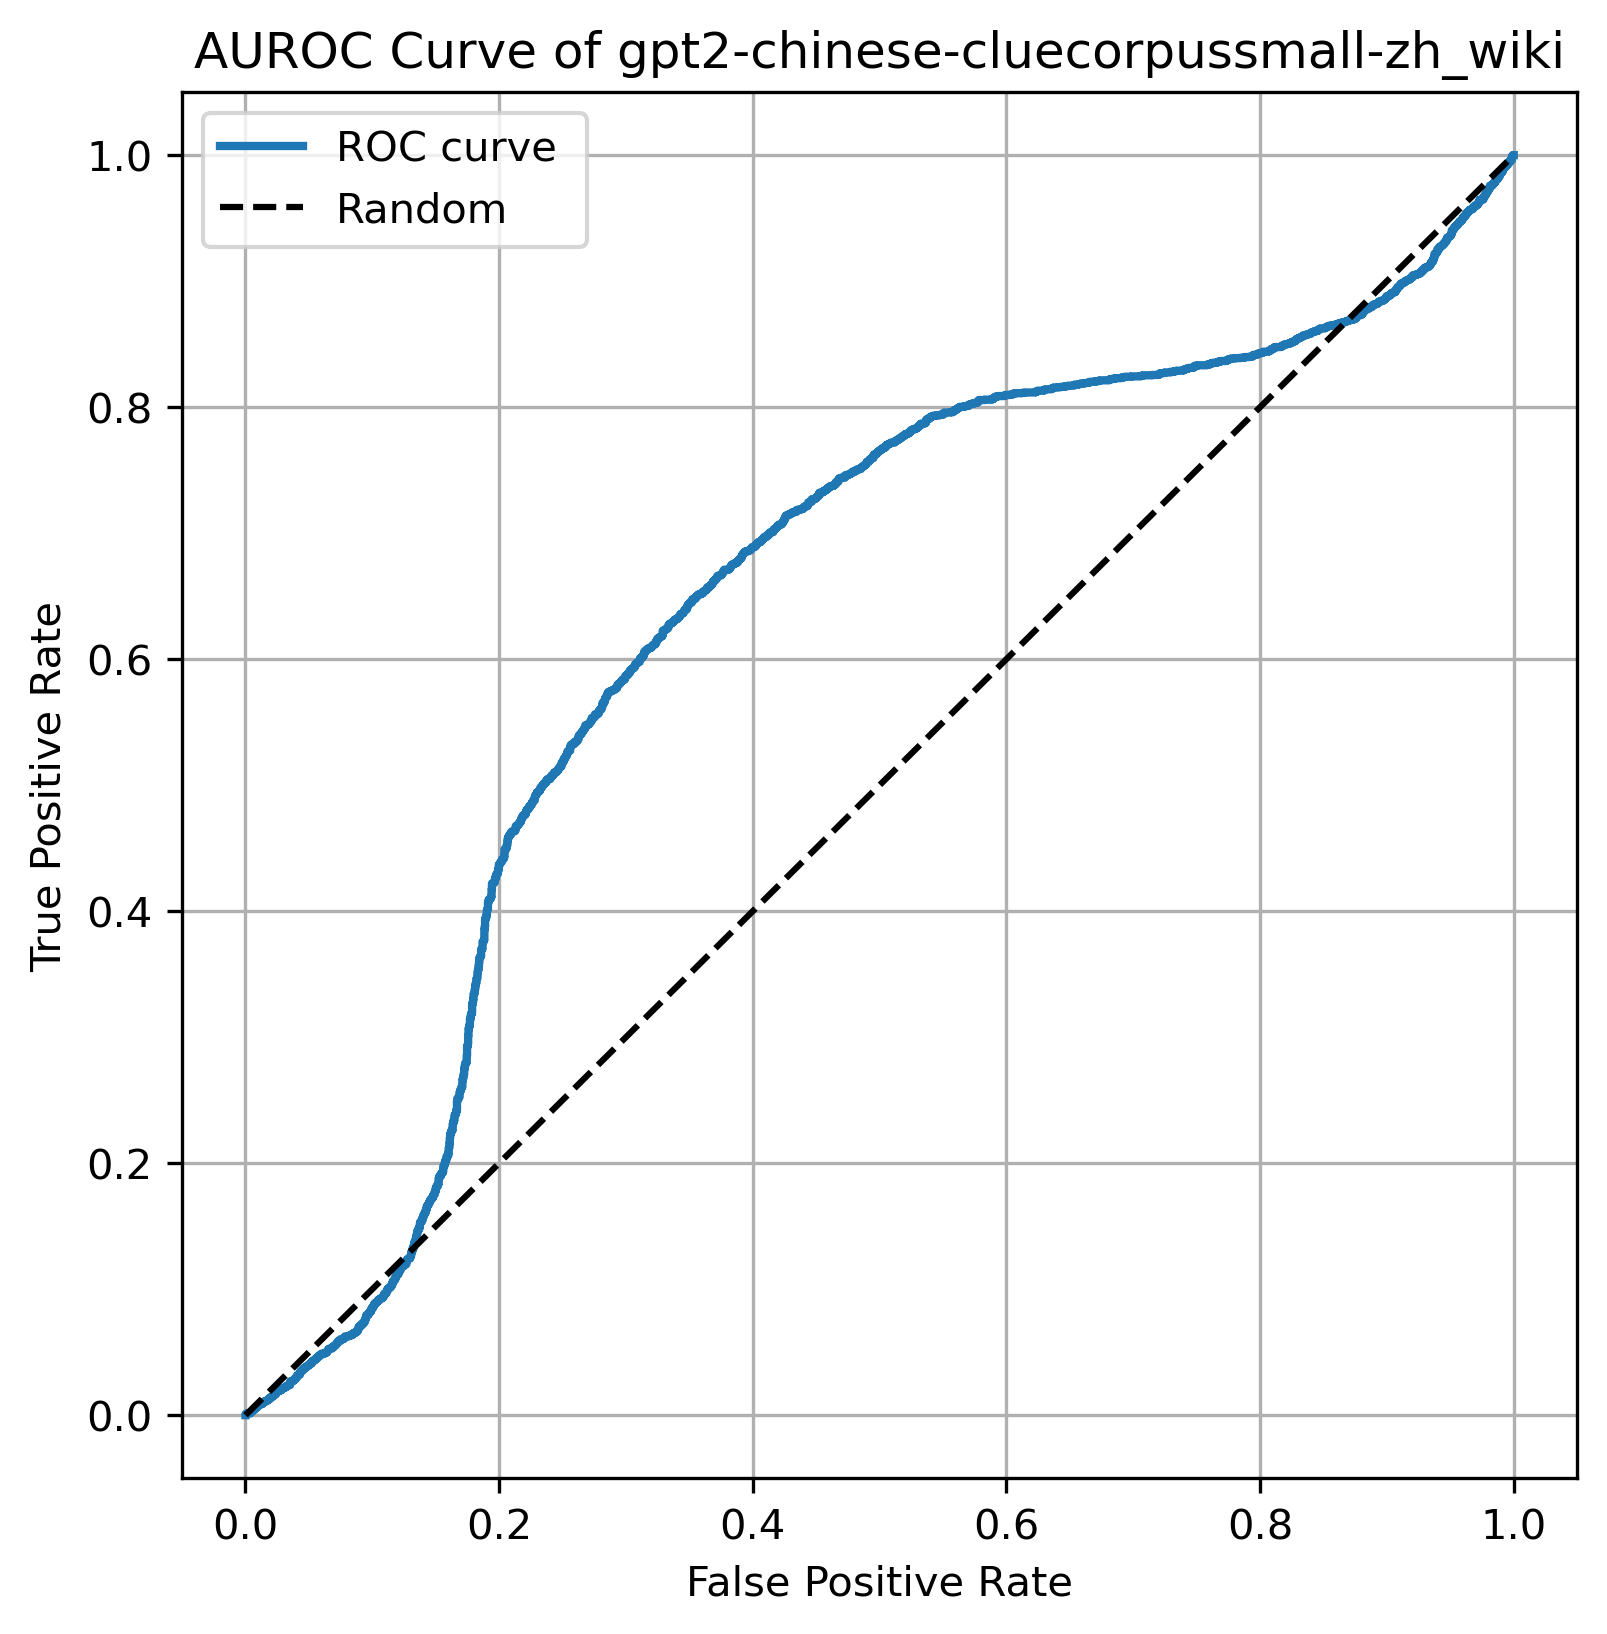
\includegraphics[width=0.3\linewidth]{images/gpt2-chinese-cluecorpussmall-zh_wiki.png}

    \vspace{0.5em}

    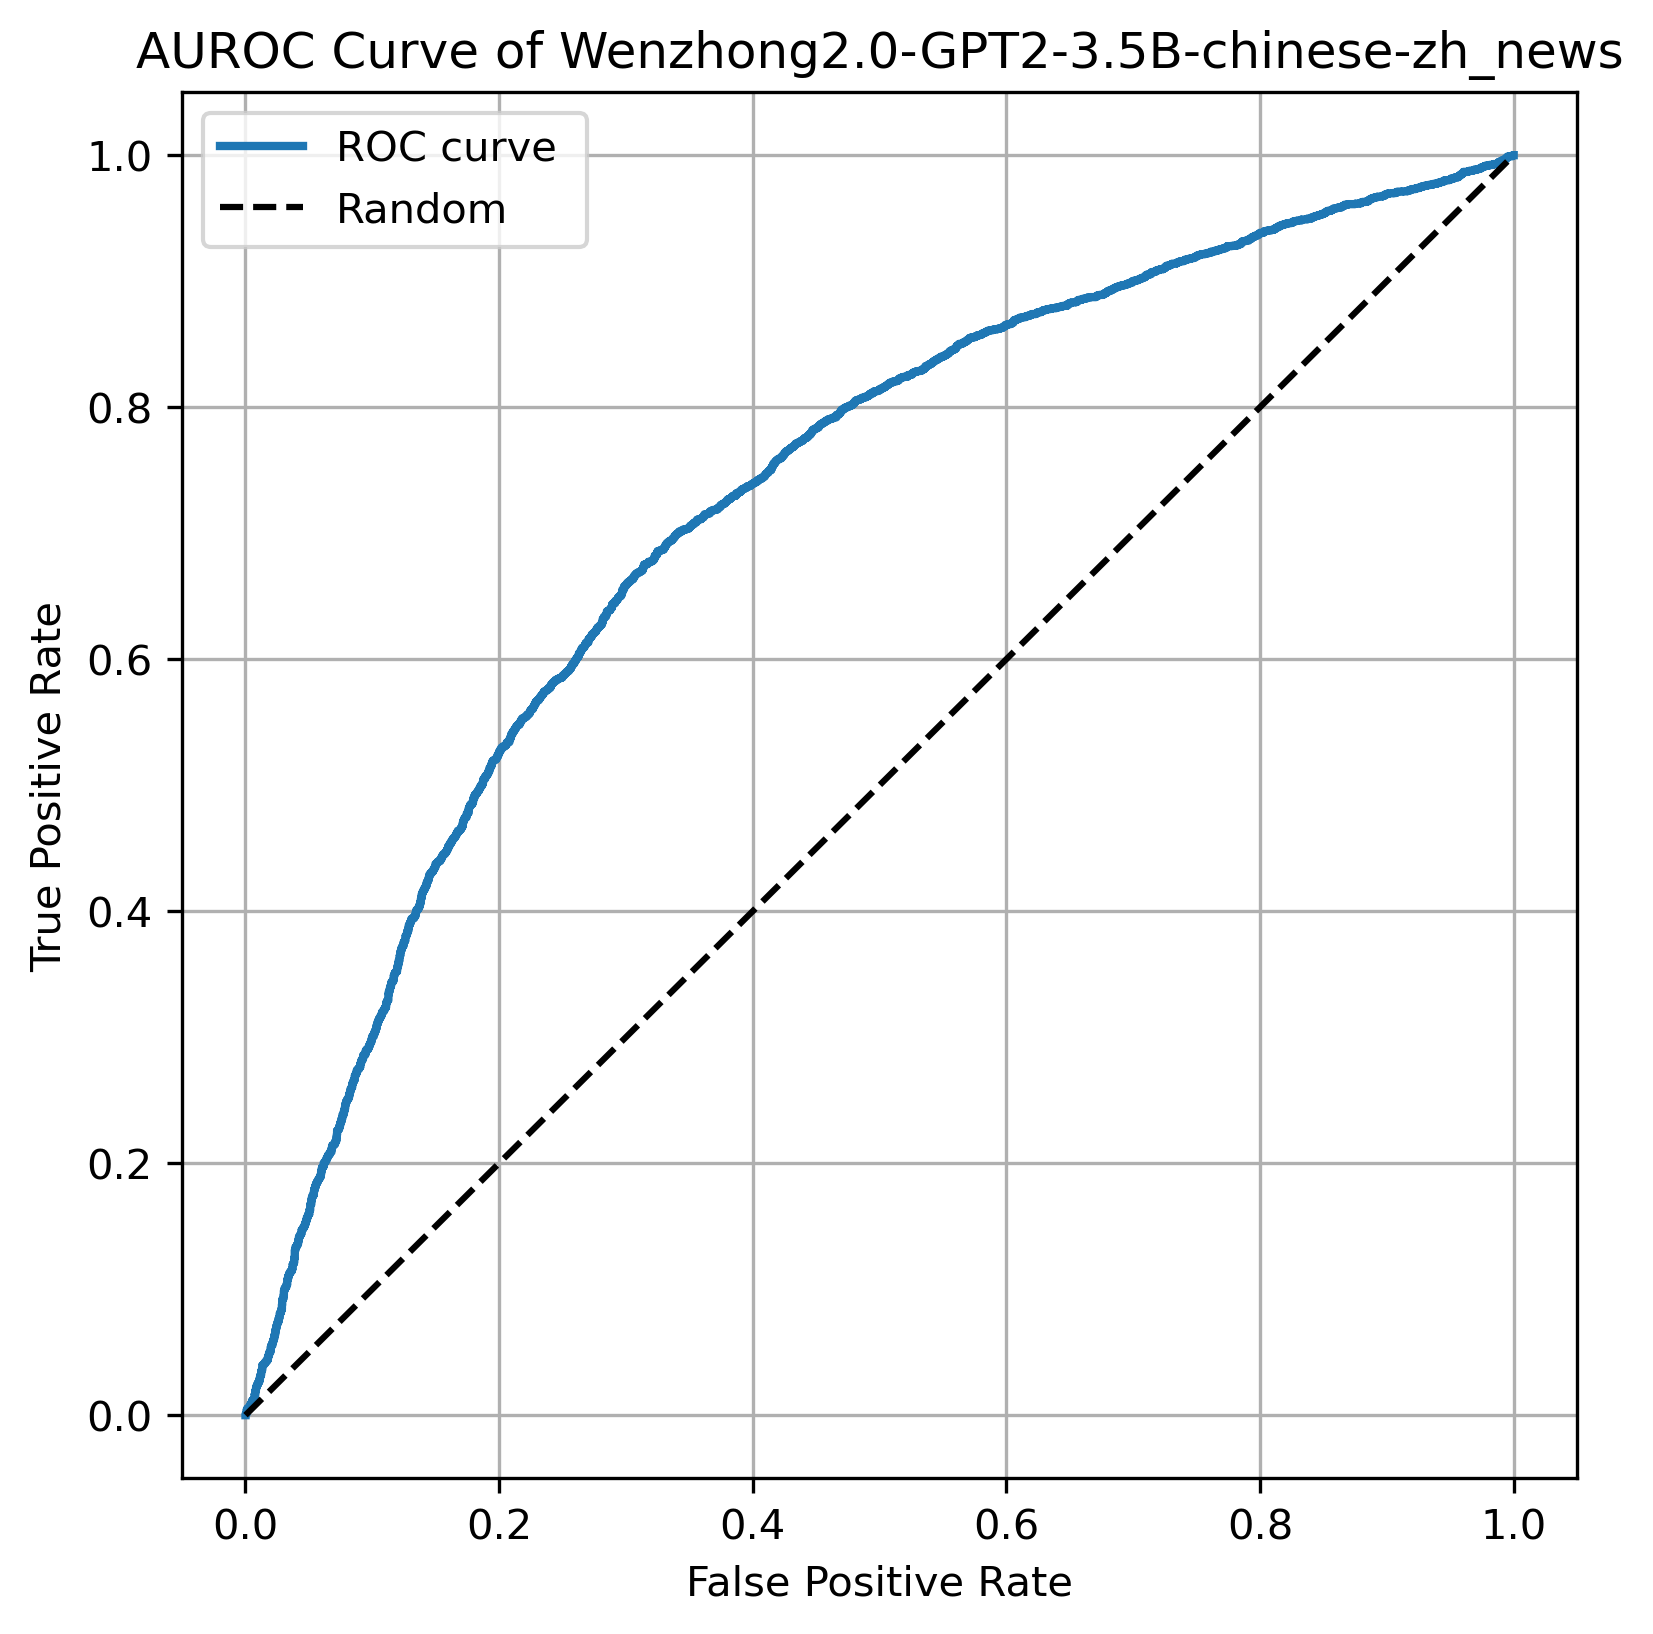
\includegraphics[width=0.3\linewidth]{images/Wenzhong2.0-GPT2-3.5B-chinese-zh_news.png}
    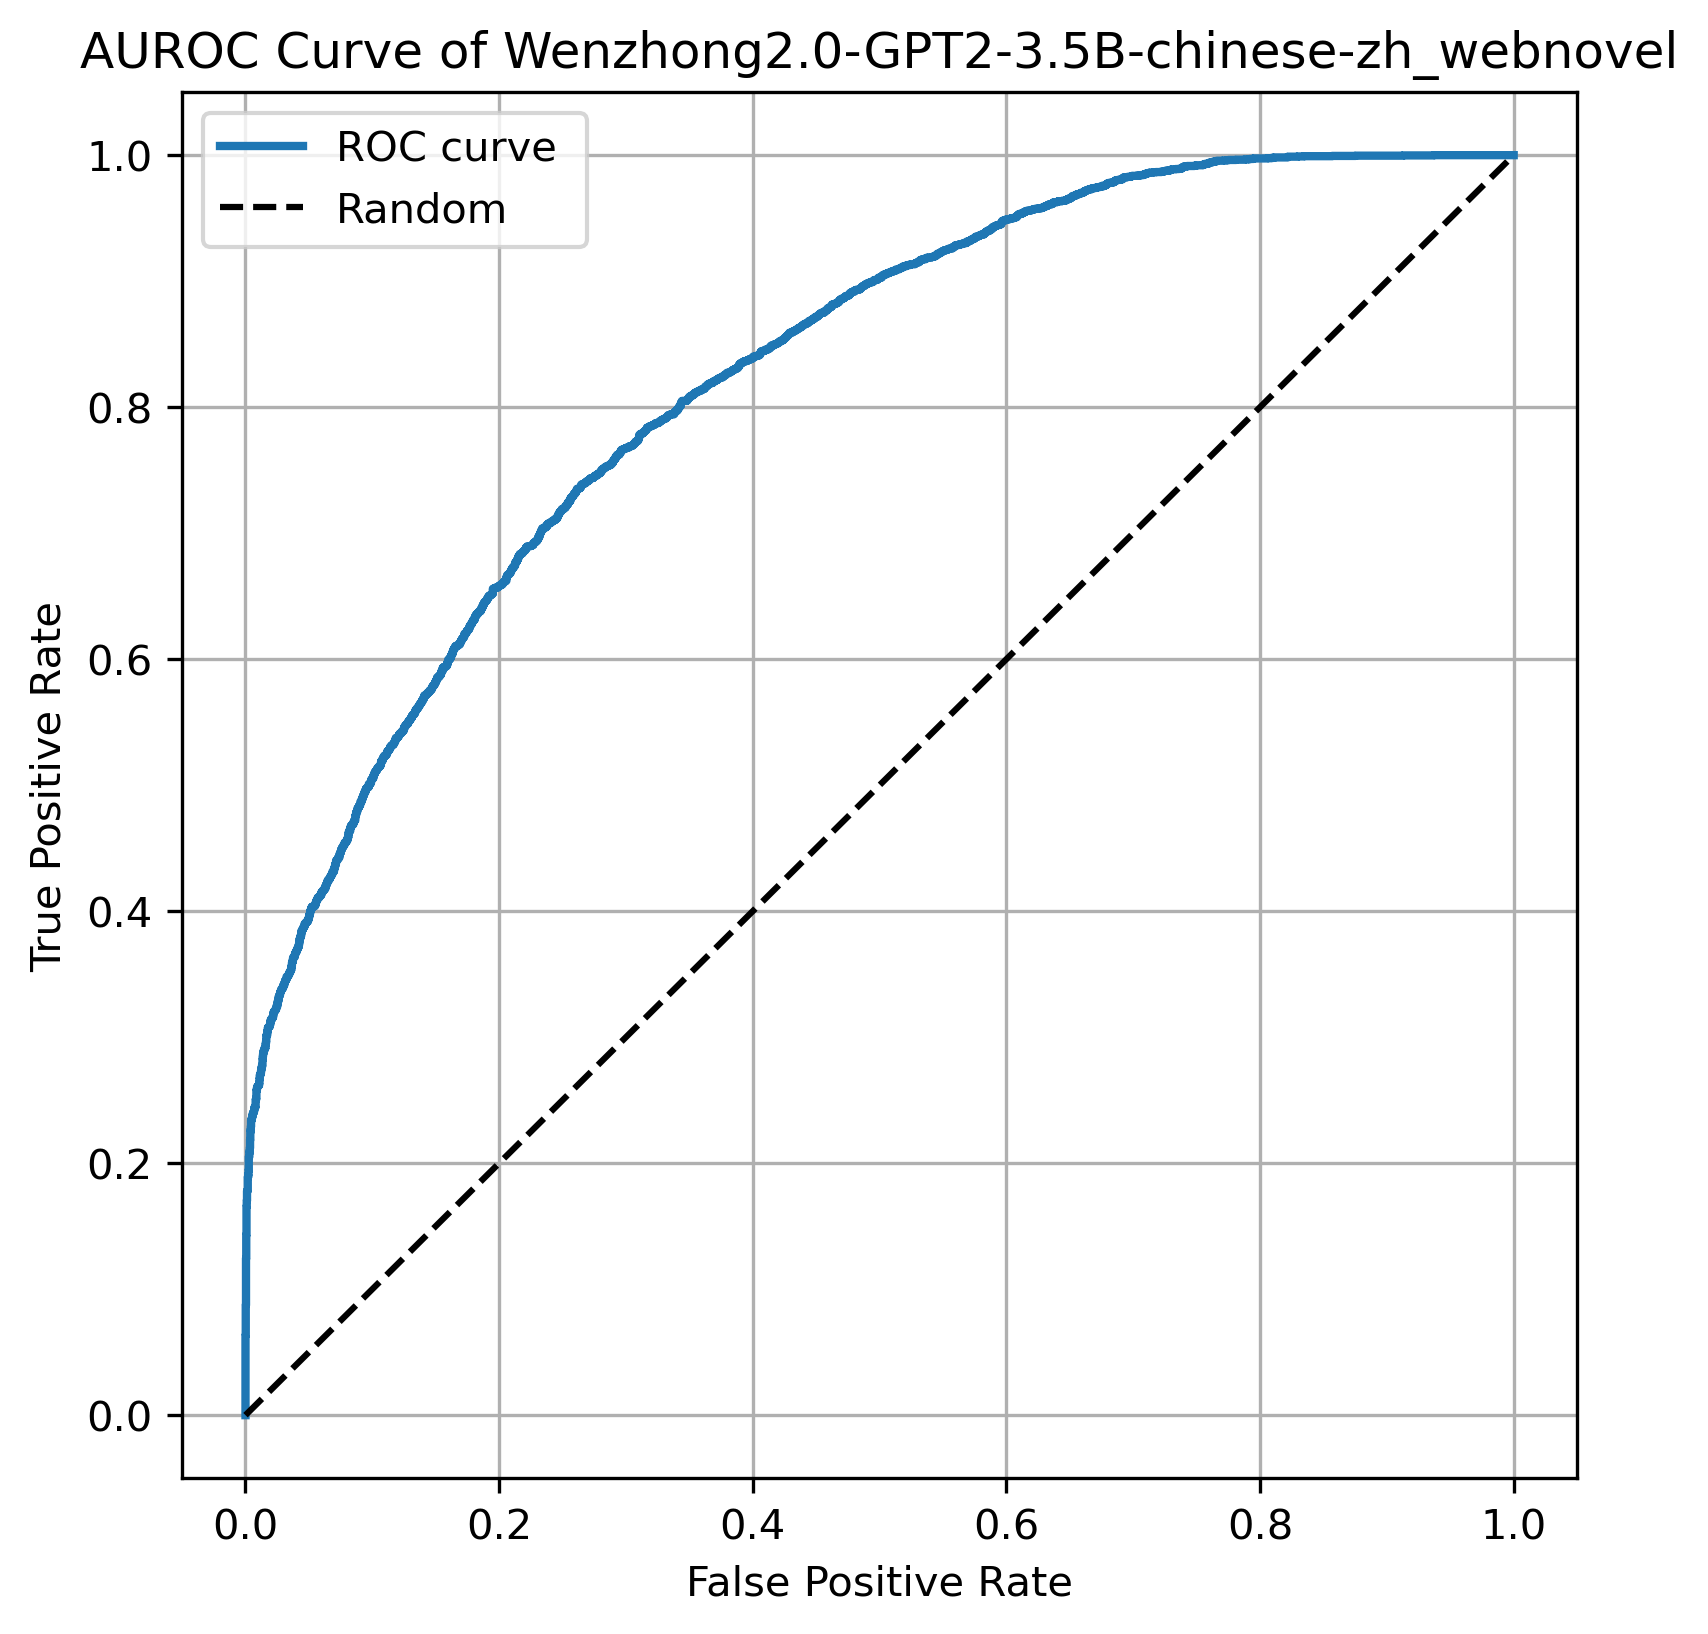
\includegraphics[width=0.3\linewidth]{images/Wenzhong2.0-GPT2-3.5B-chinese-zh_webnovel.png}
    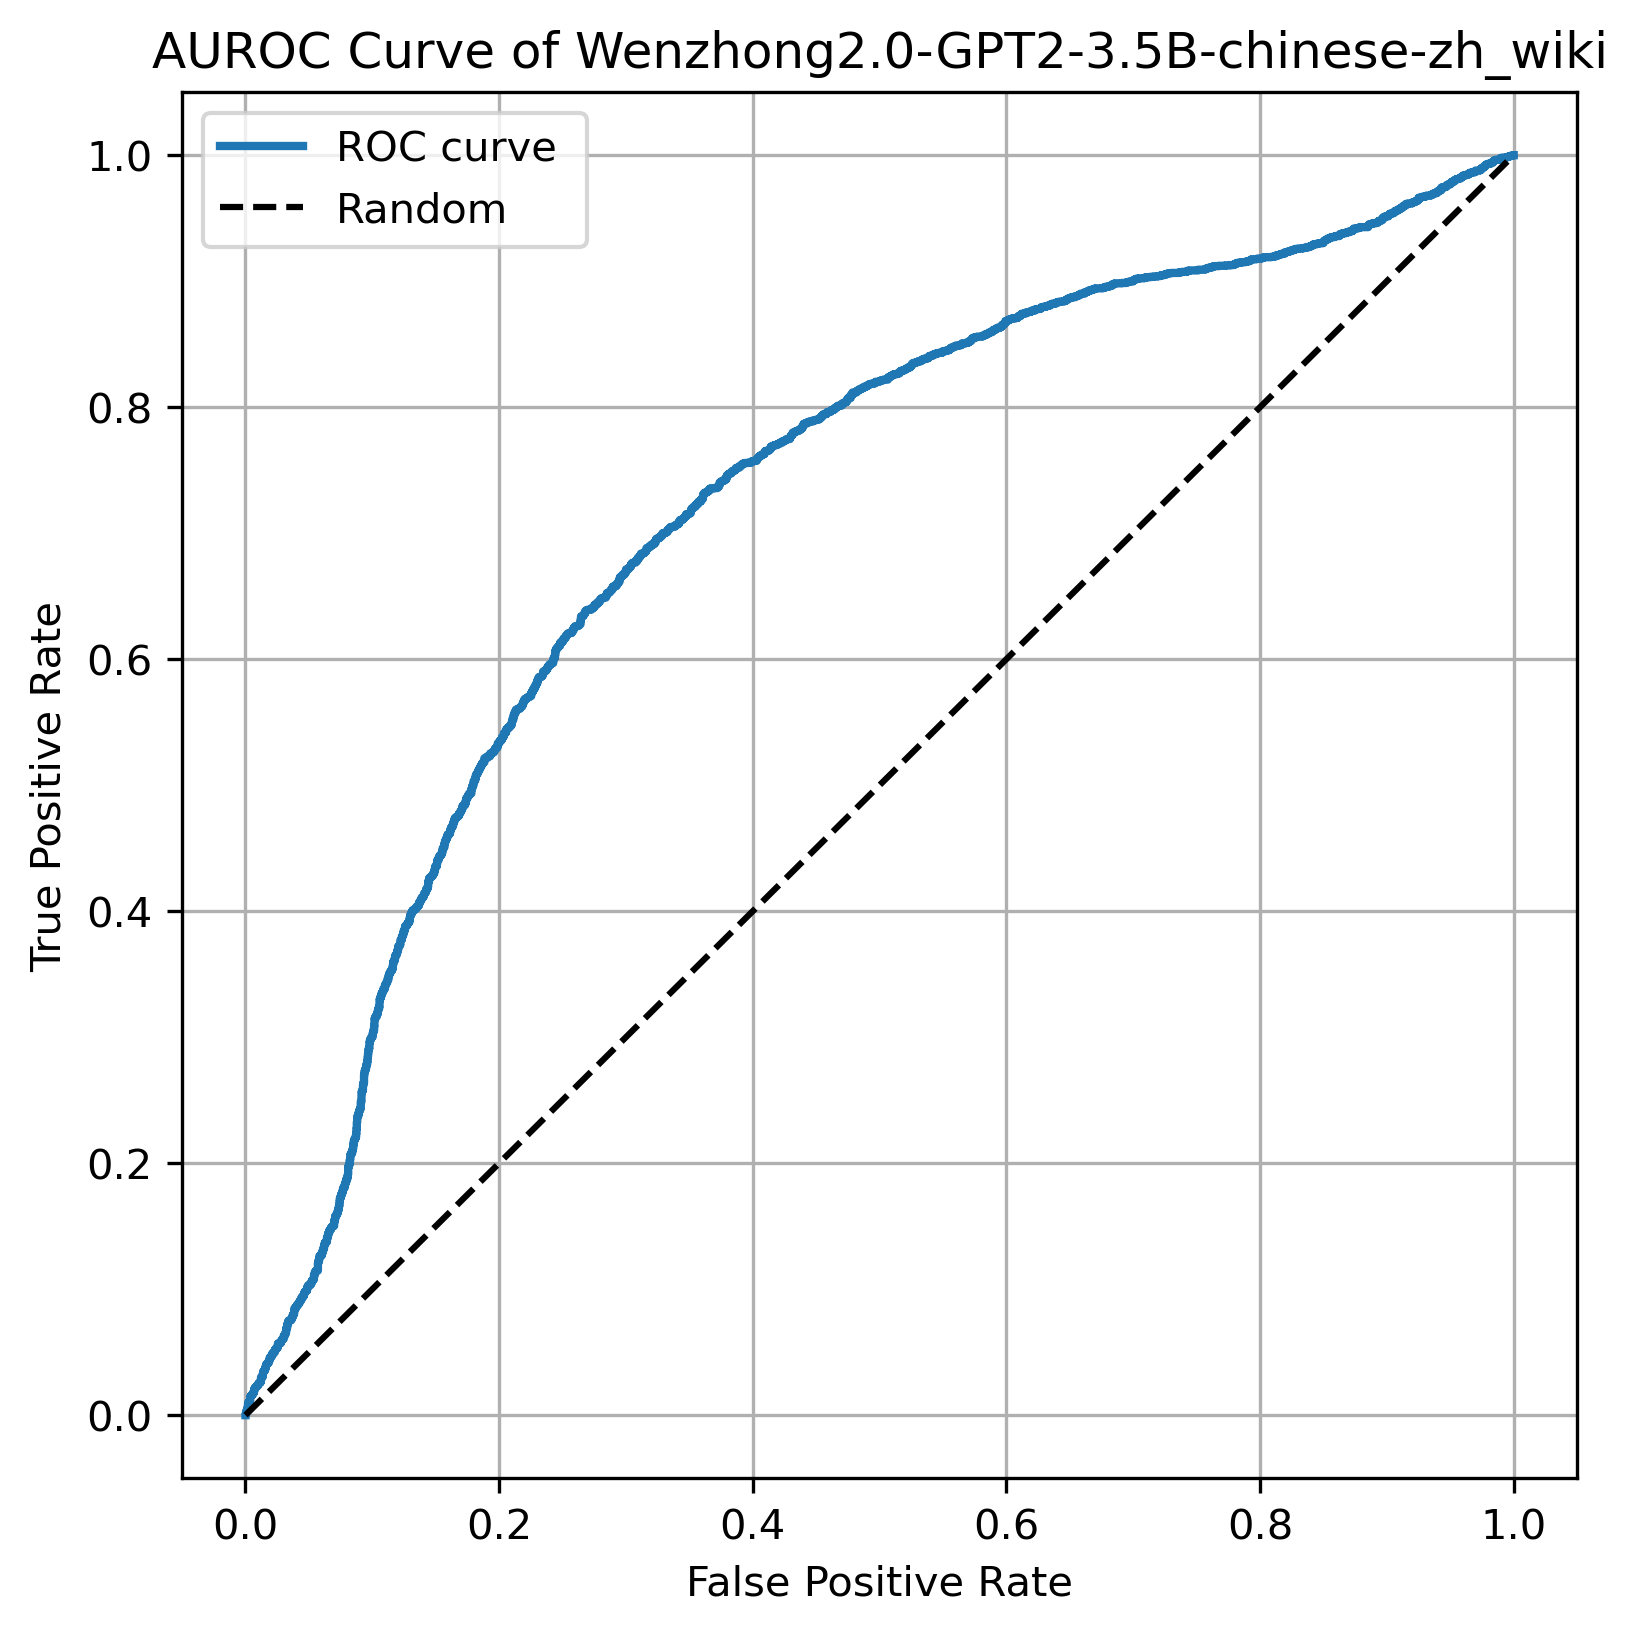
\includegraphics[width=0.3\linewidth]{images/Wenzhong2.0-GPT2-3.5B-chinese-zh_wiki.png}

    \caption{Accuracy across Chinese domains for GPT2-chinese-cluecorpussmall (top row) and Wenzhong2.0-GPT2-3.5B (bottom row) in news, webnovel, and wiki datasets.}
\end{figure}

The ROC curves for \textbf{gpt2-chinese-cluecorpussmall} exhibit a pronounced early rise in the news and webnovel datasets but remain flat and close to the diagonal in the wiki dataset, indicating weaker discrimination ability. In contrast, \textbf{Wenzhong2.0-GPT2-3.5B} demonstrates steeper and more top-left concentrated ROC curves on the news and webnovel datasets, reflecting stronger classification performance.

In the Zero-shot detection method, we compare model performance across Chinese datasets using multiple evaluation metrics.
\begin{table}[H]
 \centering
    \caption{gpt2-chinese-cluecorpussmall-Zh}
    \label{tab:my_label}
\setlength{\tabcolsep}{2pt}
\renewcommand{\arraystretch}{1.0}
\vspace{0.3cm}
\resizebox{0.4\textwidth}{!}{%
\begin{tabular}{|l|c|c|c|}
\hline
\textbf{FT domain} & \textbf{news} & \textbf{webnovel} & \textbf{wiki} \\
\hline
Accuracy & 0.6227 & 0.6821 & 0.6474 \\
\hline
AUROC & 0.6561 & 0.7933 & 0.6381 \\
\hline
\end{tabular}%
}
\end{table}



\begin{table}[H]
 \centering
    \caption{Wenzhong2.0-GPT2-3.5B-chinese-Zh}
    \label{tab:my_label}
\setlength{\tabcolsep}{2pt}
\renewcommand{\arraystretch}{1.0}
\vspace{0.3cm}
\resizebox{0.4\textwidth}{!}{%
\begin{tabular}{|l|c|c|c|}
\hline
\textbf{FT domain} & \textbf{news} & \textbf{webnovel} & \textbf{wiki} \\
\hline
Accuracy & 0.6788 & 0.7360 & 0.6849 \\
\hline
AUROC & 0.7232 & 0.8240 & 0.7216 \\
\hline
\end{tabular}%
}
\end{table}





\section{Result analysis}

\subsection{In-Domain Accuracy on English Datasets}

To evaluate different detection approaches under in-domain settings, we compare the performance of \textbf{Text Supervised Fine-Tuning, Spectral Supervised Fine-Tuning, and Spectral Zero-Shot methods on English datasets.}


\begin{figure}[H]
    \centering
    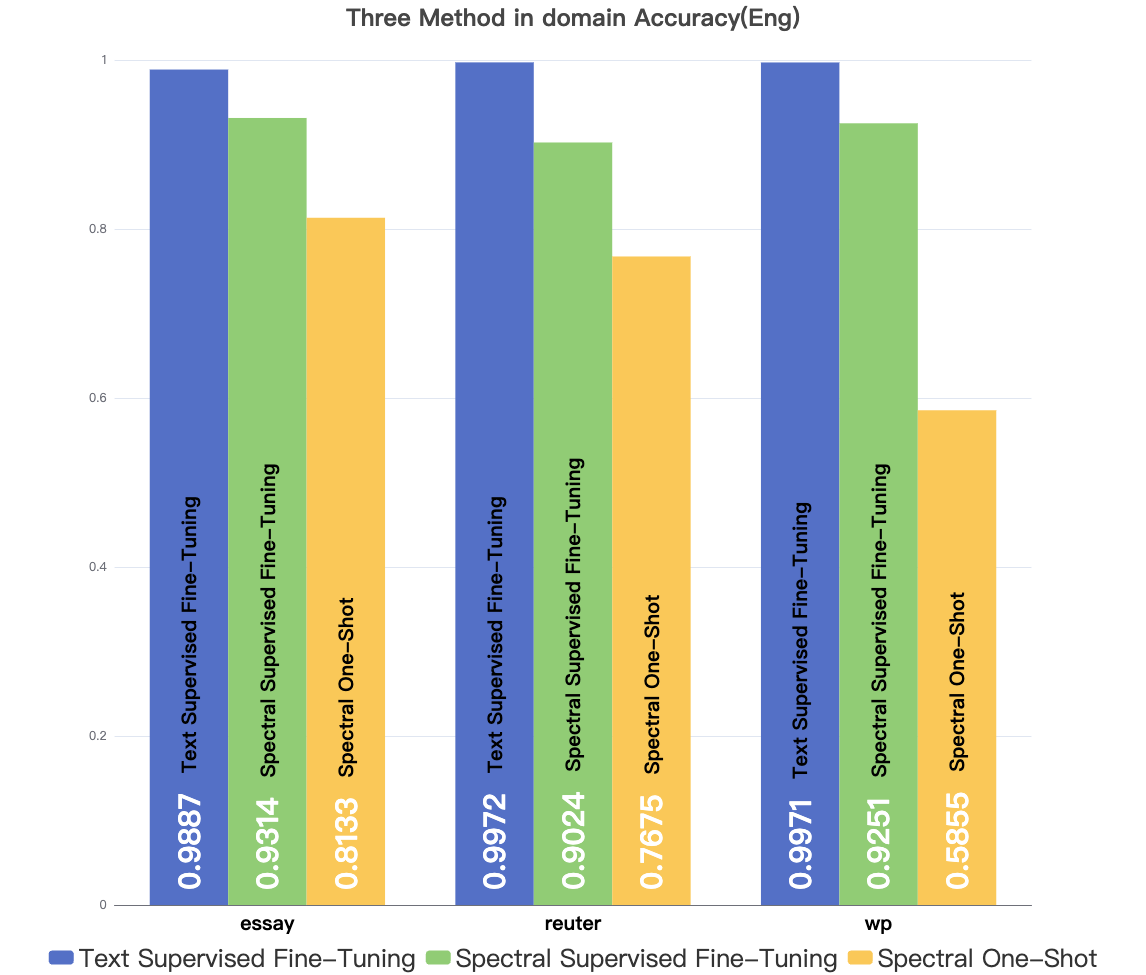
\includegraphics[width=0.65\linewidth]{images/Three Method in domain Accuracy(Eng).png}
    \caption{In-domain accuracy comparison across English datasets.}
\end{figure}


\textbf{Text Supervised Fine-Tuning achieves the highest accuracy across all domains}, demonstrating the effectiveness of direct supervision. In contrast, the \textbf{Zero-Shot method performs the worst,} with notably high sensitivity to domain variation, especially in the wp domain where its accuracy drops to 0.58.

\subsection{Out-of-Domain Accuracy on English Datasets}

We next examine how each \textbf{method generalizes} to unseen domains in the English setting.

\begin{figure}[H]
    \centering
    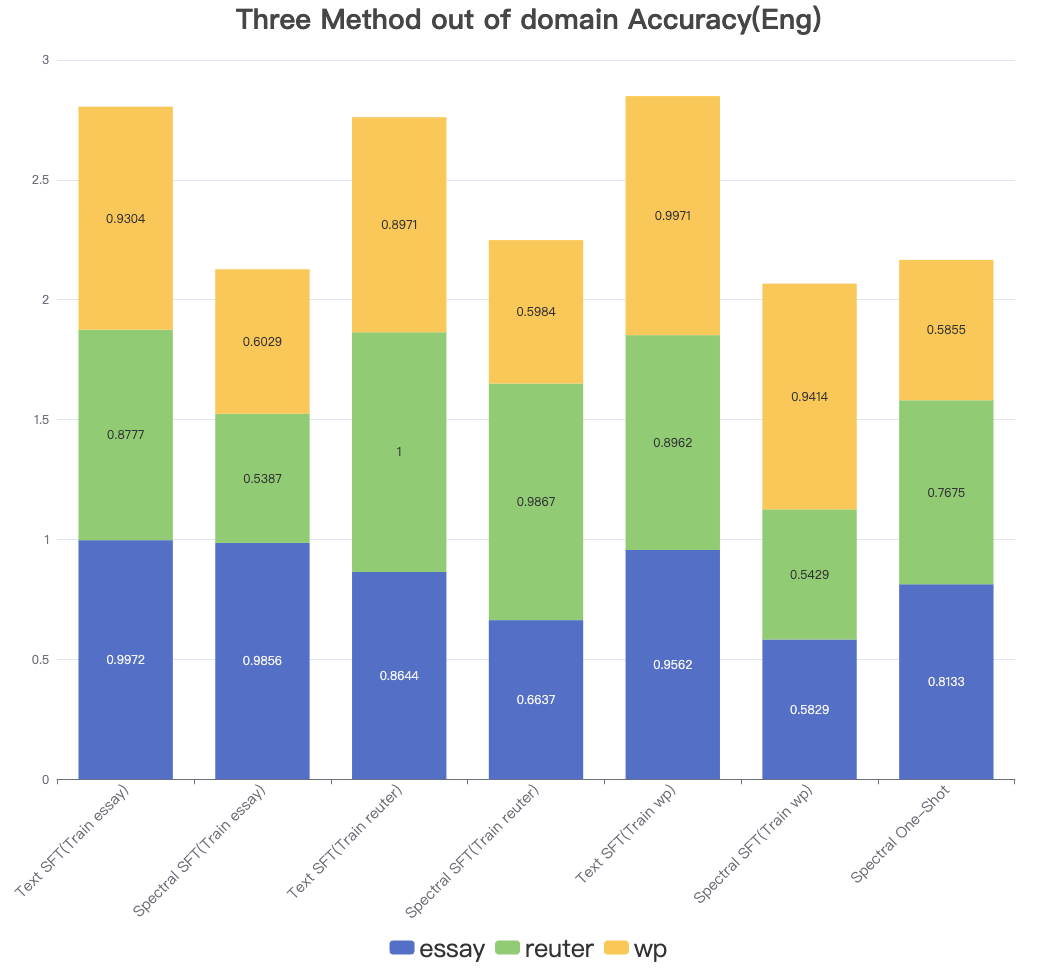
\includegraphics[width=0.65\linewidth]{images/Three Method out of domain Accuracy(Eng).png}
    \caption{Cross-domain (out-of-domain) accuracy comparison on English datasets.}
\end{figure}
\begin{table}[H]
\centering
\begin{tabular}{|l|c|c|c|}
\hline
Train on & Essay & Reuter & Wp \\
\hline
Text SFT     & 0.9972 & 0.8644 & 0.9562 \\
\hline
Spectrum SFT & 0.9856 & 0.6637 & 0.5829 \\
\hline
One-shot     & \multicolumn{3}{c|}{0.8133} \\
\hline
\end{tabular}
\caption{Cross-domain accuracy when tested on Essay (English datasets).}
\end{table}

\begin{table}[H]
\centering
\begin{tabular}{|l|c|c|c|}
\hline
Train on & Essay & Reuter & Wp \\
\hline
Text SFT     & 0.8777 & 1.0000 & 0.8962 \\
\hline
Spectrum SFT & 0.5387 & 0.9867 & 0.5429 \\
\hline
One-shot     & \multicolumn{3}{c|}{0.7675} \\
\hline
\end{tabular}
\caption{Cross-domain accuracy when tested on Reuter (English datasets).}
\end{table}

\begin{table}[H]
\centering
\begin{tabular}{|l|c|c|c|}
\hline
Train on & Essay & Reuter & Wp \\
\hline
Text SFT     & 0.9304 & 0.8971 & 0.9971 \\
\hline
Spectrum SFT & 0.6029 & 0.5984 & 0.9414 \\
\hline
One-shot     & \multicolumn{3}{c|}{0.5855} \\
\hline
\end{tabular}
\caption{Cross-domain accuracy when tested on Wp (English datasets).}
\end{table}
\textbf{Text Supervised Fine-Tuning exhibits strong cross-domain generalization,} maintaining accuracy above 0.85. However, \textbf{Spectral Supervised Fine-Tuning performs poorly in this setting}, with accuracy dropping below 0.6. Interestingly, t\textbf{he Spectral Zero-Shot method shows promising results on the essay (0.81) and reuter (0.77) domains}, highlighting its potential in specific scenarios.

\subsection{In-Domain Accuracy on Chinese Datasets}

We perform a similar evaluation for \textbf{Chinese datasets}, measuring in-domain performance of the three methods.

\begin{figure}[H]
    \centering
    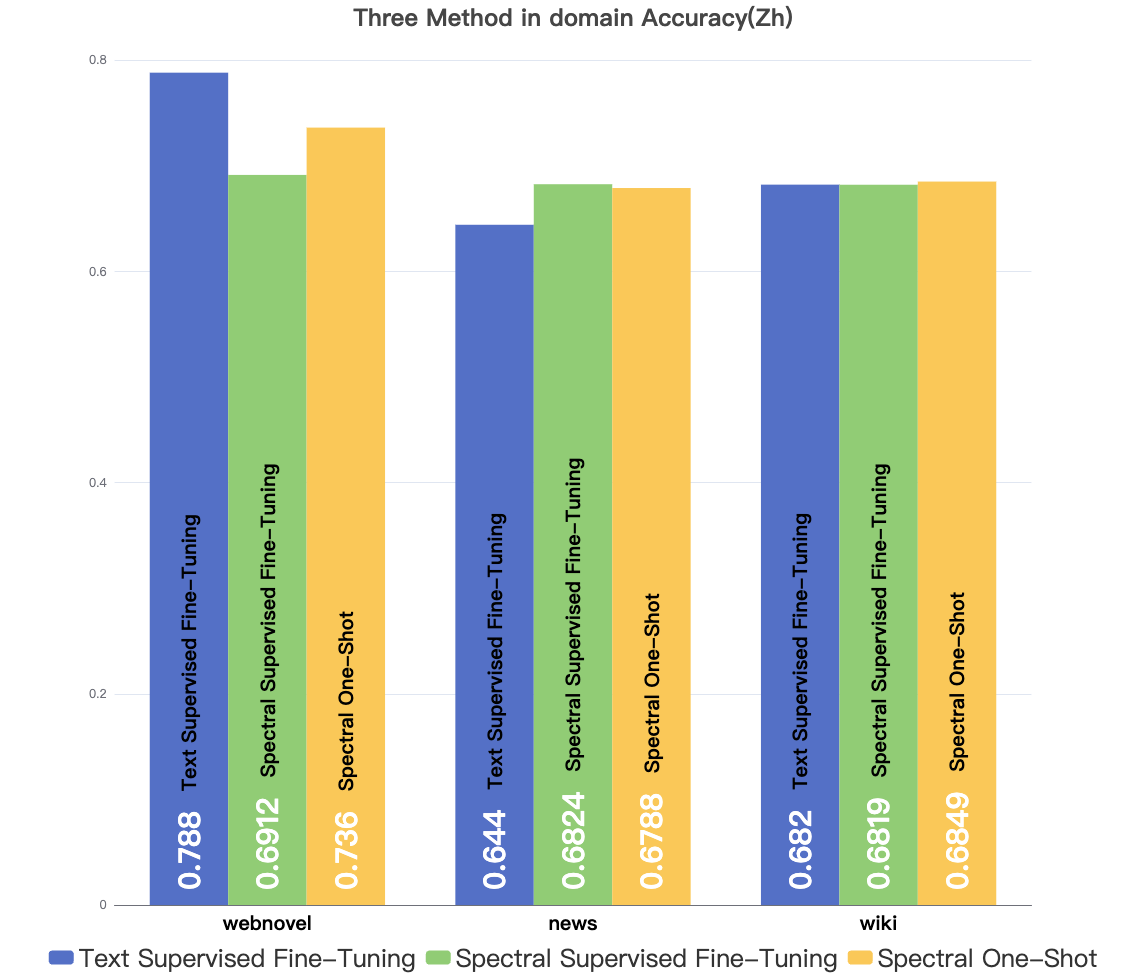
\includegraphics[width=0.65\linewidth]{images/Three Method in domain Accuracy(Zh).png}
    \caption{In-domain accuracy comparison across Chinese datasets.}
\end{figure}


\textbf{Text Supervised Fine-Tuning leads in the webnovel domain with an accuracy of 0.788}. However, the \textbf{two FourierGPT-based methods also perform competitively}, particularly in the news and wiki domains, where their accuracies remain around 0.68.

\subsection{Out-of-Domain Accuracy on Chinese Datasets}

We further assess the \textbf{cross-domain generalization ability }of each method on Chinese datasets.

\begin{figure}[H]
    \centering
    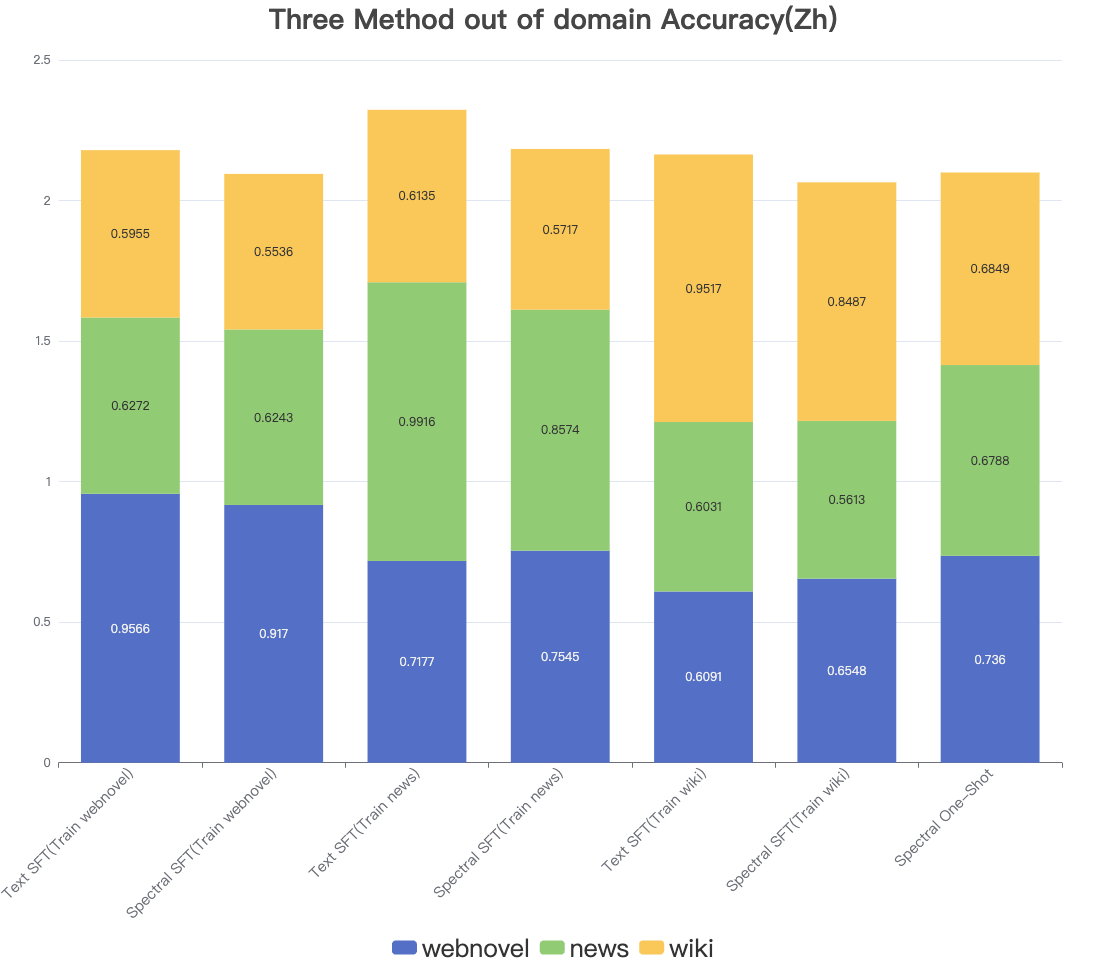
\includegraphics[width=0.65\linewidth]{images/Three Method out of domain Accuracy(Zh).png}
    \caption{Cross-domain (out-of-domain) accuracy comparison on Chinese datasets.}
\end{figure}
\begin{table}[H]
\centering
\begin{tabular}{|l|c|c|c|}
\hline
Train on & Webnovel & News & Wiki \\
\hline
Text SFT     & 0.9566 & 0.7177 & 0.6091 \\
\hline
Spectrum SFT & 0.9170 & 0.7545 & 0.6548 \\
\hline
One-shot     & \multicolumn{3}{c|}{0.6849} \\
\hline
\end{tabular}
\caption{Cross-domain accuracy when tested on Webnovel (Chinese datasets).}
\end{table}

\begin{table}[H]
\centering
\begin{tabular}{|l|c|c|c|}
\hline
Train on & Webnovel & News & Wiki \\
\hline
Text SFT     & 0.6272 & 0.9916 & 0.6031 \\
\hline
Spectrum SFT & 0.6243 & 0.8574 & 0.5613 \\
\hline
One-shot     & \multicolumn{3}{c|}{0.6788} \\
\hline
\end{tabular}
\caption{Cross-domain accuracy when tested on News (Chinese datasets).}
\end{table}

\begin{table}[H]
\centering
\begin{tabular}{|l|c|c|c|}
\hline
Train on & Webnovel & News & Wiki \\
\hline
Text SFT     & 0.5955 & 0.6153 & 0.9517 \\
\hline
Spectrum SFT & 0.5536 & 0.5717 & 0.8487 \\
\hline
One-shot     & \multicolumn{3}{c|}{0.7360} \\
\hline
\end{tabular}
\caption{Cross-domain accuracy when tested on Wiki (Chinese datasets).}
\end{table}


\textbf{Both supervised learning methods struggle in the out-of-domain scenario}, with accuracy below 0.65. In contrast, \textbf{the Zero-Shot detection method demonstrates relatively strong generalization}, maintaining performance above 0.65 across all domains.

\subsection{Reasoning}

\begin{enumerate}
    \item \textbf{Which method performs best in in-domain scenarios, and why?}
    
    \textit{Answer:} \\
   Text Supervised \textbf{Fine-Tuning consistently achieves the highest accuracy in in-domain tasks} because it enables the model to learn detailed domain-specific features and patterns, whereas \textbf{Zero-Shot} methods lack access to such labeled examples during training.
 
    \item \textbf{Which method performs best in out-of-domain (OOD) scenarios, and why?}
    
    \textit{Answer:} \\
    \textbf{Zero-Shot (One-Shot) methods show better generalization in out-of-domain settings}, especially in the \textbf{Chinese datasets}, because they do not rely heavily on domain-specific training data. Instead, they utilize more generalizable spectral features or pretrained knowledge, making them more adaptable to unseen domains despite lower in-domain accuracy.

   \item \textbf{Why do the One-Shot results differ from those reported in essay?}
   
    \textit{Answer:} \\
 Our English dataset is generated by \textbf{gpt3.5-turbo}, which uses \textbf{Reinforcement Learning from Human Feedback (RLHF)} to improve the quality and safety of its generated content by leveraging human feedback. It also undergoes specialized fine-tuning to \textbf{enhance reasoning,  maintain memory and logical consistency} in multi-turn conversations. So it's harder to discriminate it from human than GPT 3.5 which is used in the paper.
    \vspace{0.3cm}
    \item \textbf{Why do supervised methods achieve lower accuracy in Chinese compared to English?}
    
    \textit{Answer:} \\
    The lower accuracy in Chinese supervised learning is mainly due to the increased \textbf{complexity and diversity of the Chinese language}, such as rich characters and more ambiguous context. 
    \end{enumerate}



\section{Conclusion}
\subsection{Summary}
\begin{itemize}
  \item This project compares \textbf{supervised learning} and \textbf{zero-shot detection} methods for cross-domain text generation detection.
  \item \textbf{Supervised learning} achieves the best performance \textbf{in-domain}, especially with \textbf{text supervised fine-tuning}.
  \item \textbf{Zero-shot detection} demonstrates stronger \textbf{out-of-domain generalization}, particularly on Chinese datasets.
  \item The \textbf{spectrum-based methods} provide effective feature representations to enhance detection robustness.
\end{itemize}
\subsection{Future}
\begin{itemize}
  \item Explore \textbf{more advanced pretrained models}, including larger multilingual models, for detection tasks.
  \item Investigate integrating \textbf{multi-modal information} (e.g., speech, images) to improve detection accuracy.
  \item Develop \textbf{more efficient spectral analysis and feature augmentation techniques} to boost zero-shot detection performance.
  \item Expand datasets in \textbf{size and diversity}, focusing on real-world and varied text sources.
\end{itemize}


\renewcommand{\refname}{References}  % Add this line before your bibliography

\begin{thebibliography}{2}
\bibitem{xu2024}
Xu, Y., Wang, Y., An, H., Liu, Z., \& Li, Y. (2024). 
\textit{Detecting subtle differences between human and model languages using spectrum of relative likelihood}. 
arXiv preprint arXiv:2406.19874.
\end{thebibliography}

\end{document}
